%---------------------------------------------------------------------------%
%- Chapter 4: 六区的条件比较与两翼探针
%---------------------------------------------------------------------------%
\chapter{六区的条件比较与两翼探针}\label{chap:4}

%-- Section 4.1: 同一个问题怎样跨核区比较
\setcounter{section}{0}%
\IfFileExists{Tex/Sections/sec-4-1.tex}{%
    \section{同一个问题怎样跨核区比较}\label{sec:4-1}

在第~1~章中，原子核低能激发谱已被置于六个典型质量区的宏观坐标之中；第~2~章与第~3~章则进一步从微观壳模型、平均场自洽形变、对称性恢复投影以及转动、手征与摆动等集体动力学角度，奠定了多体波函数与唯象图像的数理基础。当分析视角从单个核素转向全局核素图谱时，跨核区比较往往成为检验模型泛化能力、揭示演化规律的最有力工具。然而，跨核区比较也是极易滋生虚假类比与概念滑移的区域。

最常见的认识论误区在于：仅凭某一核区发现了特定能带结构（如两条近简并带或交错低自旋带），便将质量数 $A$ 或单一唯象参数（如能级比 $E(2^+_2)/E(2^+_1)$、三轴形变角 $\gamma$ 的单一平衡值）作为排他性判据，孤立地宣布在另一区域也必定存在完全相同的物理模式。事实上，核多体系统的集体响应从来不是孤立几何形状的直接映射，而是价轨道占据、有效相互作用单极漂移、配对超流关联与自旋窗口内探针选择定则综合作用的宏观显现。本节旨在建立一套跨核区比较的物理判据与分析方法，明确哪些量子几何与多极代数是普适可迁移的，哪些微观输入与有效参数需要在新体系中重新检验。

\subsection{比较对象：内禀组态、实验室对称性与态的映射}\label{sec:4-1-1}

跨核区比较的首要前提是厘清``究竟在比较什么对象''。原子核作为自约束的有限量子多体系统，在没有外场作用的实验室参考系中，由强相互作用与电磁相互作用主导的哈密顿量在极高精度下严格具备空间旋转群 $\mathrm{SO}(3)$ 对称性、空间反演宇称 $\mathcal{P}$ 对称性以及时间反演 $\mathcal{T}$ 对称性（在此忽略微弱的弱相互作用宇称不守恒效应）。因此，实验室参考系中物理定态的基矢必定可以按确定的总角动量量子数 $I$、宇称 $\pi$ 及其磁量子数 $M$ 展开。在实际谱学实验中，测得的通常是具有确定能级位置的纯态或处于特定取向系综与统计混合的退极化布居。

自洽平均场模型中所讨论的轴对称长椭球、扁椭球或三轴椭球形状，本质上是内禀对称性破缺参考态 $|\Phi(\beta,\gamma)\rangle$ 的几何表象。内禀系中的非零四极形变参量 $(\beta, \gamma)$ 描述的是核内多核子空间密度分布的二阶各向异性关联，如第~2.4~节式~\eqref{eq:2-4-2}所引入的玻尔坐标。

然而，单一内禀态 $|\Phi(\beta,\gamma)\rangle$ 本身并非实验室物理本征态。利用角动量投影算符 $\hat{P}^I_{MK}$ 对单一内禀构型进行全欧拉角积分，所构造的仅是具备良好角动量量子数的投影试探态（trial states）：
\begin{equation}\label{eq:4-1-projection}
|IM\alpha\rangle = \sum_K g_K^\alpha \hat{P}^I_{MK} |\Phi\rangle = \sum_K g_K^\alpha \frac{2I+1}{8\pi^2} \int \mathrm{d}\Omega \, \mathcal{D}^{I*}_{MK}(\Omega) \hat{R}(\Omega) |\Phi\rangle.
\end{equation}
在物理真实的有限核系统中，实际定态通常是多个具有不同形变构型、配对自由度或准粒子激发的内禀态的多体量子叠加（例如生成坐标法 GCM 或多参考能量泛函理论所描述的构型混合网络）。

这意味着，跨核区比较的对象绝不能停留在某个未投影平均场势能面（PES）局域极小点的坐标数值上，而必须落实到经对称性恢复后具有确定自旋与宇称的物理态 $|I^\pi\rangle$、这些态之间的跃迁网络以及波函数在形变构型空间上的概率分布。在波函数分布极其弥散的大振幅软核中，实验室一体电荷密度对于 $0^+$ 基态处处呈现球对称，唯有通过高阶两体密度关联与电磁多极约化矩阵元，方能提取内部形状的客观物理实在性\cite{poves-2020-limits-assigning-nuclear-shape}。

\subsection{微观驱动与动力学响应：轨道占据、单极演化与配对关联}\label{sec:4-1-2}

比较本文所选的核与自旋区间时，一个重要差别是费米面附近的轨道及其占据。以下是相关案例中的轨道线索；同一质量数附近仍可有不同的质子数、中子数与组态。
\begin{itemize}
\item 在 $A\approx 60$ 与 $80$ 区域，质子与中子费米面主要受 $1f_{5/2}, 2p_{3/2}, 2p_{1/2}$ 以及下落的 $1g_{9/2}$ 独特宇称轨道主导；
\item 在 $A\approx 130$ 区域，中子接近壳层中上部，质子位于准空穴或下部，负宇称独特轨道 $1h_{11/2}$ 的驱动效应成为主导；
\item 在 $A\approx 160$ 稀土重区，强形变长椭球势阱将 $1i_{13/2}$ 轨道大幅劈裂；
\item 在 $A\approx 190$ 区域，费米面则深埋于 $1i_{13/2}$ 中子空穴与 $1h_{9/2}, 2f_{7/2}$ 混合轨道之中。
\end{itemize}

在给定高 $j$ 壳层与近轴对称参考中，不同 $|\Omega|$ 分量具有不同的四极矩，粒子与相对于满壳定义的空穴也可给出相反贡献。费米面移动改变这些分量的占据，并通过残余相互作用与核芯极化反馈改变形变倾向。但单个 $K$ 或 $\Omega$ 标签不能独自决定长椭、扁椭或三轴形状；还需核对具体 Nilsson 能级随形变的变化、配对和相互作用。第~2.2~节的占据反馈提供了这种比较的微观出发点\cite{book-bohr-mottelson-nuclear-structure-vol2}。

更深层次的微观驱动还来自于多核子相互作用中的单极效应（monopole interaction）。正如第~2.2~节式~\eqref{eq:2-2-1}所展开的单极相互作用分解与有效单粒子能量（ESPE）演化框架所示，随着价核子在不同组态间的填充或跃迁，核子间张量力与自旋-同位旋交换相互作用引起有效能隙的动态漂移\cite{doctoral-r1-g28-otsuka-2023-type-ii-shell-evolution}。在跨区比较中，这种单极演化逻辑展现出鲜明的核区特性：例如在 $A\approx 100$ 区域，正是质子从 $2p, 1f$ 轨道激发至 $1g_{9/2}$ 时，通过强烈的单极吸引作用诱发了中子 $1g_{7/2}$ 与 $1h_{11/2}$ 轨道的突变性下移，形成了所谓的第二类壳演化（Type-II shell evolution）与形变自强化反馈\cite{doctoral-r1-g28-togashi-2016-zr-mcsm-qpt}；而在高质子数区，这种单极诱导相变的临界核子数则发生显著位移。

配对关联通过改变占据、准粒子能量和响应矩阵元调制转动惯量。在指定平均场的比较中，配对常使低频响应相对无配对参考减小；这不构成各轴惯量与经典刚体值之间的普遍不等式。第~2.6~节区分了冻结场与含残余响应的实现。不同核或组态的单粒子谱、配对和顺排过程不同，跨区比较时应重新检验这些输入。

\subsection{形变空间测度与高阶不变量：$\gamma$ 刚性、$\gamma$ 软性与分布宽度}\label{sec:4-1-3}

三轴自由度是跨区比较中最易引起混淆的概念之一。在唯象模型中，人们常将 Davydov-Filippov 刚性三轴转子模型与 Wilets-Jean $\gamma$ 不稳定模型进行对照：
\begin{itemize}
\item \textbf{刚性三轴假设}：设想势能面在非零三轴平衡角（如 $\gamma \approx 20^\circ\text{--}30^\circ$）处具有较深而局域的极小，波函数集中于极小点近旁；
\item \textbf{$\gamma$ 软性/不稳定假设}：势能面沿 $\gamma$ 方向展现宽平坦特性，核波函数在整个三轴区间广泛弥散，不存在静态固定的三轴取向。
\end{itemize}

指定的理想刚性转子与 $\gamma$ 不稳定模型可以给出不同的能级和跃迁预言，应逐项比较。在更一般的势能与惯量可调模型中，少数能级对反问题的约束仍可能不足。因此不能把某个能比当作形状分布的唯一测量，也不能把拟合的非唯一性误写成两个理想极限的完整能谱相同。

第~2.1、2.4~节给出了 Kumar--Cline 不变量的实验室张量定义\cite{cline-1986-nuclear-shapes-coulomb-excitation}。标量求和不需预先选定转子势，几何解释则仍遵循所声明的坐标、算符与截断条件。对 $0^+$ 态，沿用同一归一可写：
\begin{equation}\label{eq:4-1-q2-invariant}
P_2\equiv q_2=\langle Q^2\rangle=\sqrt5\langle0_i^+|[\mathcal M(E2)\times\mathcal M(E2)]_0|0_i^+\rangle=\sum_t|\langle2_t^+\Vert\mathcal M(E2)\Vert0_i^+\rangle|^2,
\end{equation}
\begin{equation}\label{eq:4-1-q3-invariant}
P_3\equiv q_3=\langle Q^3\cos3\gamma\rangle=-\sqrt{\frac{35}{2}}\langle0_i^+|[\mathcal M(E2)\times[\mathcal M(E2)\times\mathcal M(E2)]_2]_0|0_i^+\rangle.
\end{equation}
这里的几何解释沿用第~2.1、2.4~节的坐标与算符条件；原作形状角 $\delta$ 的记号须与本文辐射混合比分开。更高阶不变量可约束相应算符矩的涨落，但从这些矩到连续角度分布仍需额外假设，不能仅由四阶四极矩直接读出角度方差。

然而必须保持审慎的证据边界：低阶几何不变量 $\langle Q^2 \rangle$ 与 $\langle Q^3 \cos 3\delta \rangle$ 仅提供了宏观形状电荷分布的二阶与三阶矩重心，并不能唯一反演核多体波函数在 $(\beta,\gamma)$ 连续坐标空间上的全概率分布密度。更重要的是，实验测得的 $E2$ 矩阵元网络总是有限截断的，高能中间态的缺失与矩阵元相对符号的不确定性会引入系统误差。因此，分散度参数能够为检验多体模型波函数提供关键约束，但绝不能将其简化为某种机械数值门槛去绝对化地判定刚性或软核。

\subsection{实验探针与观测选择定则：自旋窗口、激发机制与电磁张量算符}\label{sec:4-1-4}

跨区比较结论的可信度，高度受制于所采用实验探针的布居物理机制及其自旋-宇称选择定则。不同实验手段在核素图上所能触及的激发能量与自旋窗口存在显著差异：
\begin{enumerate}
\item \textbf{低自旋、高精度绝对跃迁探针}：
   低能库仑激发、$\beta$ 衰变、中子俘获与NRF具有不同的形成机制和选择规则。中子俘获还涉及复合核，不能统称为纯电磁微扰探针。可达自旋由实际入射道、母态及级联决定；相应矩阵元或率的提取还需效率、分支、寿命或反应模型等输入，不能给这一组方法规定统一的低自旋上限。
\item \textbf{中高自旋在束反应探针}：
   包括重离子熔合蒸发反应（Heavy-Ion Fusion-Evaporation）、深部非弹性碰撞（Deep Inelastic Collisions）、多核子转移反应以及自发/诱发裂变碎块谱学。这类探针通过大角动量输入能够有效布居高自旋转动带，是探索高自旋带交叉、磁转动剪刀带、手征双重带及摆动激发的有力工具。然而，必须注意不同反应机制的角动量输入截面与退激统计分布截然不同；且多步库仑激发在重区强形变核中同样可以达到 $I \sim 20\text{--}30$ 的高自旋态。绝对跃迁强度的测定不仅依赖反冲距离法（RDDS）和多普勒频移衰减法（DSAM），还广泛依赖于电子学超快计时（如 $\mathrm{LaBr}_3(\mathrm{Ce})$ 阵列）、延迟符合、转化电子谱学以及 NRF 共振荧光线宽分析等互补技术。
\end{enumerate}

不同观测量约束波函数的不同侧面，其区分能力取决于待检验解释与实验误差，不存在普遍的信息量排名：
\begin{itemize}
\item \textbf{能级能量 $E(I)$}：约束哈密顿量与态混合，有时对交叉和能隙尤为敏感；当多个模型已用这些能量调参时，还需留出观测检验；
\item \textbf{跃迁强度 $B(E2)$ 与静四极矩 $Q_s$}：前者含非对角约化矩阵元的模平方和初态统计权，后者约束对角矩阵元；二者提供互补的电荷四极信息；
\item \textbf{$\rho^2(E0)$、同位素与异能态位移}：$E0$约束同核态间的径向跃迁矩阵元，位移比较相应电荷半径期望值。结合指定构型模型可限制混合与半径差，但不由单一量唯一重建形状；
\item \textbf{单核子转移反应与单粒子谱强}：实验直接测量的物理量是反应微分截面 $\mathrm{d}\sigma/\mathrm{d}\Omega$。提取单粒子光谱因子 $S_j$ 需要引入光学势畸变波波恩近似（DWBA）或绝热转移模型，其数值不仅依赖于反应动力学势的选择，还受限于实验激发能量分辨率以及截断窗口内的碎片求和；正如第~2.2~节所讨论的，单核子转移截面反映的是核多体波函数与单粒子试探算符的重叠，不能将其误解为裸算符的一体直接测量。
\end{itemize}

\subsection{可迁移规律与需重新检验条件的物理判据：六区比较总表}\label{sec:4-1-5}

基于上述微观机制与实验物理剖析，在跨质量区核结构比较中，必须严格区分普适可迁移的理论法则与不可无条件迁移的局域输入：
\begin{itemize}
\item \textbf{可迁移的物理法则}：
  \begin{enumerate}
  \item 空间旋转与反演对称性的量子几何代数：Wigner-Eckart 定理的约化张量定义、Clebsch-Gordan 系数相位与 Racah 重耦合代数\cite{book-suhonen-from-nucleons-to-nucleus}；
  \item 电磁辐射场多极展开与跃迁几率的基本微观定义；
  \item 模型无关的 Kumar-Cline 四极不变量理论框架与零动量标量积完备求和规则\cite{cline-1986-nuclear-shapes-coulomb-excitation}；
  \item 态混合与微观组态干涉的代数分析方法。
  \end{enumerate}
\item \textbf{不可直接迁移的局域物理条件}：
  \begin{enumerate}
  \item 具体单粒子轨道的有效单粒子能量（ESPE）与局部主壳能隙；
  \item 价空间截断所引入的模型空间有效电荷（$e_p^{\mathrm{eff}}, e_n^{\mathrm{eff}}$）与有效弱轴矢流重整化因子 $g_A^{\mathrm{eff}}$；
  \item 唯象模型（如 IBM、PRM、玻尔哈密顿量 5DCH）通过局部能谱拟合所得的势能形状参数、微观质量张量或刚体转动惯量；
  \item 某一特定核区因特定高 $j$ 独特轨道单粒子耦合产生的复杂带结构（如手征双重带），在另一核区轨道占据与三轴极小尚未独立确立前，绝不能仅凭能谱外貌相似直接类推存在相同模式。
  \end{enumerate}
\end{itemize}

根据此项比较判据，表~\ref{tab:4-1-six-regions-framework}系统梳理了六个典型质量区的核心物理驱动、主导费米面轨道、关键形变特征以及当前实验认知的确定性边界。在全书后续比较论述中，我们将严格遵守表中关于``明确测定''、``未见''、``未搜索''与``灵敏度不足''四类认识论边界的界定，绝不以跨区类比掩盖物理认知的真实空缺。

\begin{table}[htbp]
\centering
\small
\setlength{\tabcolsep}{2.5pt}
\caption{以本文所选案例为线索的六区比较；质量区不是互斥的模式分类，模型解释与直接报告量分别使用}\label{tab:4-1-six-regions-framework}
\begin{tabularx}{\textwidth}{p{1.5cm}p{3.5cm}p{3.6cm}X}
\toprule
质量区 & 主导轨道与占据特征 & 核心物理机制与现象 & 实验证据与认知边界 \\
\midrule
$A \approx 60$ & 所选Ge、Ni中的壳间激发与轨道占据 & 组态混合、次闭壳效应与不同形状的模型解释 & $^{64}\mathrm{Ge}$ 寿命与E2已测；$^{68}\mathrm{Ni}$ 的低能态寿命、E2与E0上限共同约束三形状解释 \\
\addlinespace
$A \approx 80$ & 所选Kr、Ge及奇奇核的价轨道占据与核芯响应 & 形状混合、四极涨落与取向候选须分核、分态比较 & Kr带符号矩约束混合；作者以Ge高阶不变量讨论刚性；As、Br问题见第4.5节 \\
\addlinespace
$A \approx 100$ & 所选Zr模型中的占据反馈及Mo、Ru的不同响应 & 急变、软性和多极响应可出现在不同态与能窗 & Zr寿命与模型比较；Mo低能态和相对分支；Ru报告偶极强度并结合模型提出八极解释 \\
\addlinespace
$A \approx 130$ & 所选质子轨道与中子粒子或空穴的组态组合 & 手征、摆动、进动及软核耦合的条件比较 & Pr、Ce等核已报告不同候选，须分别核对能带、绝对率和所用模型 \\
\addlinespace
$A \approx 160$ & 高 $j$ 轨道与多准粒子构型；Lu案例涉及 $\pi i_{13/2}$ & 大形变转动、高 $K$ 异能态及配对与顺排响应 & Lu的TSD带提供摆动比较基准；稀土高 $K$ 跃迁须按实际支路与禁戒度比较 \\
\addlinespace
$A \approx 190$ & 所选核接近闭壳区，粒子或空穴占据随核素而变 & 扁椭、三轴、形状混合及单粒子描述的交界 & Hg、Ir、Os、Au案例按自旋窗、组态、跃迁强度与竞争解释比较 \\
\bottomrule
\end{tabularx}
\end{table}
%
}{%
    \section{同一个问题怎样跨核区比较 [未完成]}\label{sec:4-1}%
    \textit{本节尚未完成。}%
}

%-- Section 4.2: 轻区与$A\approx 80$的形状混合
\setcounter{section}{1}%
\IfFileExists{Tex/Sections/sec-4-2.tex}{%
    \section{轻区与A80的形状混合}\label{sec:4-2}

在第~4.1~节所确立的跨区比较判据中，首要原则是将抽象的代数对称性与微观核子占据和具体的实验室可观测量严格锚定。沿核素图向中等质量区推进，$A\approx 60$ 与 $A\approx 80$ 区域（主要涵盖 $\mathrm{Ni}$、$\mathrm{Ge}$、$\mathrm{Se}$ 与 $\mathrm{Kr}$ 等同位素）展现出全核素图谱中极为剧烈、演化迅速的形状共存与构型混合现象。在这些核中，低激发谱上频繁出现反常的低激发 $0^+_2$ 态、强烈交错的能带结构以及受阻或增强的电磁跃迁。

然而，实验上观察到低激发 $0^+$ 态或非谐振动能级，绝不能简单断言体系必定存在多个具有深势垒隔离的宏观几何极小（即经典意义上的多形状共存）。本节将从两态混合的微观代数出发，依托 $^{68}\mathrm{Ni}$、$^{64}\mathrm{Ge}$、$^{74,76}\mathrm{Kr}$ 与 $^{76}\mathrm{Ge}$ 等经典实验原件，剖析电单极跃迁强度 $\rho^2(E0)$、静四极矩 $Q_s$ 的测量条件与 Kumar-Cline 四极几何不变量在检验模型中的实际角色，并明确与奇奇核手征-反射多重带的分工接口。

\subsection{两态与多态混合模型：能谱退化与物理可观测量}\label{sec:4-2-1}

理解形状共存与构型混合的最简洁物理起点是两态混合模型。设多体希尔伯特空间中存在两个未微扰的正交基矢 $|0^+_A\rangle$ 与 $|0^+_B\rangle$，它们分别对应具有不同内禀形变几何（例如一者为近球形或长椭球，另一者为扁椭球或大形变组态）的非微扰构型。设未微扰本征能量满足 $E_A \le E_B$，残余相互作用在两个构型之间诱发常数非对角耦合矩阵元 $V$（约定 $V > 0$）。

包含耦合的多体哈密顿量在基矢 $\{|0^+_A\rangle, |0^+_B\rangle\}$ 下写为：
\begin{equation}\label{eq:4-2-two-state-H}
\mathcal{H} = \begin{pmatrix} E_A & V \\ V & E_B \end{pmatrix}.
\end{equation}
对角化该哈密顿矩阵，物理观测到的两个正交定态 $|0^+_1\rangle$ 与 $|0^+_2\rangle$ 可表述为：
\begin{equation}\label{eq:4-2-two-state-states}
\begin{aligned}
|0^+_1\rangle &= \cos\theta_0 |0^+_A\rangle + \sin\theta_0 |0^+_B\rangle, \\
|0^+_2\rangle &= -\sin\theta_0 |0^+_A\rangle + \cos\theta_0 |0^+_B\rangle.
\end{aligned}
\end{equation}
要求物理定态之间非对角能量矩阵元严格消失，即
\begin{equation*}
\langle 0^+_1 | \mathcal{H} | 0^+_2 \rangle = \frac{1}{2}(E_B - E_A)\sin 2\theta_0 + V\cos 2\theta_0 = 0 ,
\end{equation*}
由此给出混合角与未微扰能隙的精确关系：
\begin{equation}\label{eq:4-2-two-state-mixing}
\Delta E = \sqrt{(E_B - E_A)^2 + 4V^2}, \qquad \tan 2\theta_0 = -\frac{2V}{E_B - E_A}.
\end{equation}
在 $E_A<E_B$、$V>0$ 时取 $-\pi/4<\theta_0<0$；当 $E_A=E_B$ 且 $V>0$ 时，连续极限为 $\theta_0=-\pi/4$。若能量相同且 $V=0$，二态空间简并，单凭哈密顿量不能固定混合角。

给定观测能隙 $\Delta E$，未扰动差 $(E_B-E_A)$ 与 $V$ 仍有多组解。混合大小由相对比例 $2V/(E_B-E_A)$ 决定：即使 $V$ 的绝对值很小，只要未扰动差更小，混合也可很强。二态能量拟合还不说明这两个基底是否对应彼此分离的形状极小；确定几何解释需要更多观测与模型条件。

电单极跃迁（Electric Monopole, $E0$）提供另一类约束。这里取点质子电荷算符 $\hat T(E0)=e\sum_{p=1}^{Z}r_p^2$，坐标相对核质心；每质子平均均方半径为 $\langle r^2\rangle_{A/B}=Z^{-1}\langle 0^+_{A/B}|\sum_p r_p^2|0^+_{A/B}\rangle$。除基底正交外，再假设该基底的非对角单极矩阵元可忽略；后一个假设不由正交性自动推出。由此得到：
\begin{equation}\label{eq:4-2-e0-matrix}
\langle 0^+_2 | \hat{T}(E0) | 0^+_1 \rangle = eZ\sin\theta_0\cos\theta_0\left(\langle r^2\rangle_B-\langle r^2\rangle_A\right).
\end{equation}
两个物理态之间的约化单极跃迁强度 $\rho^2(E0)$ 定义为无量纲比值：
\begin{equation}\label{eq:4-2-rho-e0-diff}
\rho^2(E0; 0^+_2 \to 0^+_1) \equiv \frac{|\langle 0^+_2 | \hat{T}(E0) | 0^+_1 \rangle|^2}{e^2 R_0^4} = \frac{1}{4} Z^2 \sin^2(2\theta_0) \frac{\left[ \Delta\langle r^2 \rangle_{\mathrm{intr}} \right]^2}{R_0^4},
\end{equation}
式中 $R_0=1.2A^{1/3}\,\mathrm{fm}$ 是所用参考半径。这个二态近似的 $\rho^2(E0)$ 约束混合因子与半径差平方的乘积：非零值需要二者均非零，给定强度却不能分别唯一确定混合角与半径差。半径差可与形变变化相关，具体关联仍须由构型模型检验。

\subsection{68Ni与64Ge：次闭壳破缺、寿命测定与形状证据边界}\label{sec:4-2-2}

在 $A\approx 60\text{--}70$ 区域，$^{68}\mathrm{Ni}$ 与 $^{64}\mathrm{Ge}$ 构成了理解微观壳层破缺与形状共存判定界限的典型案例。

$^{68}\mathrm{Ni}$（$Z=28, N=40$）质子处于闭壳，中子填满 $1f_{5/2}, 2p_{3/2}, 2p_{1/2}$ 轨道，其费米面恰位于 $N=40$ 次闭壳。早期谱学曾根据较高的第一激发 $2^+_1$ 态能量（2033 keV）将其视作良好球形核。然而后续实验逐渐揭示出复杂的低能激发现象。Crider 等（2016）\cite{crider-2016-68ni-shape-coexistence}利用 $\beta$ 衰变谱学结合超快计时技术，对 $^{68}\mathrm{Ni}$ 的高能态与低激发态进行了寿命与分支比测量。核对 Crider 等（2016）原件 Table 1：
\begin{itemize}
\item 第一激发 $0^+_2$ 态位于 1605 keV，属于长寿命异能态（文献采用半衰期 $T_{1/2} = 268(12)\,\mathrm{ns}$），其向基态通过纯 $E0$ 内转换电子退激，采用强度为 $\rho^2(E0; 0^+_2 \to 0^+_1) \times 10^3 = 7.6(4)$；
\item Crider 等（2016）在该工作中重点测定了第二激发 $0^+_3$ 态（2511 keV）的寿命，测得其半衰期为亚纳秒量级的 $T_{1/2} = 0.57(5)\,\mathrm{ns}$；
\item 该 $0_3^+$ 态到 $2_1^+$ 的分支大于0.981，相应 $B(E2)=39.0(34)\,e^2\mathrm{fm}^4$。Table 1对其到基态及 $0_2^+$ 的E0强度仅给上限，分别为 $\rho^2(E0)<0.0050$ 和 $<0.0258$；这些上限不是测得的非零强度。
\item 同文对 $^{70}\mathrm{Ni}$ 候选 $(0_2^+)$ 采用或测定的量须单独列出：半衰期为 $1.65^{+0.30}_{-0.25}\,\mathrm{ns}$，到 $2_1^+$ 的E2分支大于0.66，而到基态的E0仅给上限。不能将其与 $^{68}\mathrm{Ni}$ 的另一态合成一次测量。
\end{itemize}
作者比较LNPS壳模型与采用A3DA相互作用的MCSM，将 $^{68}\mathrm{Ni}$ 的 $0_1^+$、$0_2^+$、$0_3^+$ 分别与球形、扁椭和长椭构型联系起来。这是模型对态结构的解释。原文第4页还列出 $0_3^+$ 的半衰期预言：A3DA与LNPS分别约108 ns和1.5 ns，与实测半衰期0.57(5) ns不同。能级和形状标签相近的模型仍可给出差异很大的绝对率，寿命因而提供另一项检验，而不能单独当作形状的直接成像。

在自共轭核 $^{64}\mathrm{Ge}$（$N=Z=32$）中，证据边界同样需要严格澄清。Starosta 等（2007）\cite{doctoral-r1-g26-starosta-2007-64ge-rdm-e2}利用单中子敲出反应 $^{9}\mathrm{Be}(^{65}\mathrm{Ge}, ^{64}\mathrm{Ge}+\gamma)X$ 结合反冲距离多普勒频移法（RDM），系统测定了低自旋态的寿命。核对原件 PDF 第 3 页 Table I 及表下说明：
\begin{itemize}
\item 第一激发 $2^+_1$ 态（902 keV）的实测平均寿命为 $\tau(2^+_1) = 3.3(5)\,\mathrm{ps}$，向下跃迁几率为 $B(E2; 2^+_1 \to 0^+_1) = 410(60)\,e^2\mathrm{fm}^4$；
\item 第二激发 $2^+_2$ 态（1579 keV）的实测平均寿命为 $\tau(2^+_2) = 8^{+4}_{-2}\,\mathrm{ps}$，向下跃迁几率分别为 $B(E2; 2^+_2 \to 2^+_1) = 620(210)\,e^2\mathrm{fm}^4$ 以及强烈受阻的交叉跃迁 $B(E2; 2^+_2 \to 0^+_1) = 1.5(5)\,e^2\mathrm{fm}^4$；
\item 原文Table I把静四极矩 $Q(2_1^+)$、$Q(2_2^+)$ 列在GXPF1A理论计算栏；这些数值不能写成该次寿命实验直接测得的静矩。
\item 原文作者据此给出的物理结论是``$^{64}\mathrm{Ge}$ 呈现集体 $\gamma$ 软非谐振动特征''。
\end{itemize}
因此，强 $B(E2)$ 证明了核内存在显著的四极集体性，但在缺乏对角静矩实测与高阶不变量的情况下，绝不能把理论预测列当成实验实测值，更不能将该核直接当作已经实验证实的多形状共存。

\subsection{74,76,78Kr：多步库仑激发、能带混合与静四极矩测量}\label{sec:4-2-3}

在氪（$\mathrm{Kr}$）同位素链中，随着中子数向中子亏损一侧推进，势能面表现出强烈的长椭与扁椭竞争。由于实验室系中 $0^+$ 基态由角动量守恒定理决定其一阶静四极矩严格为零（$\langle 0^+ | \hat{Q}_{20} | 0^+ \rangle \equiv 0$），内禀电荷各向异性的对角信息在低自旋下主要体现于带内激发态（如 $2^+_1, 2^+_2$）的静四极矩 $Q_s$ 中。

根据第2.1节限定于轴对称 $K=0$ 带的几何关系，对于纯轴对称长椭构型（$Q_0 > 0$），基态带 $2^+_1$ 态的静四极矩预期为负值（$Q_s(2^+_1) < 0$）；而对于扁椭构型（$Q_0 < 0$），则预期为正值（$Q_s(2^+_1) > 0$）。然而在实际原子核中，由于构型混合的存在，观测到的定态静矩是各基矢分量矩阵元的相干叠加。

Clément 等（2007）\cite{doctoral-r1-g27-clement-2007-prc-krypton-coulex}在 GANIL/SPIRAL 装置上，利用放射性束 $^{74}\mathrm{Kr}$ 与稳定束 $^{76}\mathrm{Kr}$ 轰击 $^{208}\mathrm{Pb}$ 靶进行了多步安全库仑激发，通过 GOSIA 程序拟合求解了包含数十个能级矩阵元的网络。查阅 Clément 等（2007）原件表格：
\begin{itemize}
\item 在 $^{76}\mathrm{Kr}$ 中，原件 PDF 第 11 页 Table VI 列出的实验结果为：$2^+_1$ 态的静四极矩为 $Q_s(2^+_1) = -0.7(2)\,e\mathrm{b}$（约化矩阵元 $\langle 2^+_1 || M(E2) || 2^+_1 \rangle = -0.9(3)\,e\mathrm{b}$）；
\item 在更缺中子的 $^{74}\mathrm{Kr}$ 中，原件 PDF 第 15 页 Table XI 列出的实验拟合结果为：$2^+_1$ 态的静四极矩为 $Q_s(2^+_1) = -0.53^{+0.24}_{-0.23}\,e\mathrm{b}$（约化矩阵元 $\langle 2^+_1 || M(E2) || 2^+_1 \rangle = -0.70^{+0.31}_{-0.30}\,e\mathrm{b}$）。
\end{itemize}
由此可见，实验直接测得的 $^{74}\mathrm{Kr}$ 与 $^{76}\mathrm{Kr}$ 第一激发 $2^+_1$ 态的静四极矩测量中心值\textbf{均为负值}，并非网络文献或二手笔记中所误传的一正一负数值。

那么 Clément 等是如何确立两核中存在长椭与扁椭形状共存的？其论证并非建立在单个静矩的孤立符号上，而是基于两能带混合模型（two-band mixing model）对全能带跃迁矩阵元与能级的全局自洽拟合：
\begin{itemize}
\item 在未微扰表象中，假定存在一个长椭带和一个扁椭带；
\item 全局拟合表明，在 $^{76}\mathrm{Kr}$ 中，未微扰基态带由长椭构型主导，长椭构型处于能量低端；
\item 而在 $^{74}\mathrm{Kr}$ 中，未微扰能隙发生反转，未微扰扁椭构型的带头能量低于长椭构型带头；通过强烈的带间混合矩阵元（$V \approx 330\,\mathrm{keV}$），混合后的物理基态具有显著的未微扰扁椭成分（约占 $50\%\text{--}60\%$），而物理激发带则与长椭构型强烈交织。
\end{itemize}
这一严密的原始证据表明：形状反转与共存的判定依赖于包含多个态跃迁与静矩的完整混合模型反演，绝不能用对角单态静矩的简单符号去代替能带波函数的复杂混合。

\subsection{72,74,76Ge：刚性三轴 vs 软势竞争与Kumar-Cline不变量提取}\label{sec:4-2-4}

在锗（$\mathrm{Ge}$）同位素链中，物理探讨的核心聚焦于势能面的三轴刚性与 $\gamma$ 软性。

Ayangeakaa 等（2019）\cite{ayangeakaa-2019-rigid-triaxial-ge76}利用 GRETINA 阵列结合 CHICO2 探测器，对 $^{76}\mathrm{Ge}$ 实施了多步库仑激发，在有限能级范围内拟合了电磁矩阵元网络，并结合采用的寿命、分支等约束。该工作采用 Kumar-Cline 几何不变量方法（见式~\eqref{eq:4-1-q2-invariant}与式~\eqref{eq:4-1-q3-invariant}），提取了四极变形不变量 $\langle Q^2 \rangle$ 以及三轴不变量 $\langle Q^3 \cos 3\delta \rangle$。核对原件 PDF 第 5–6 页：该工作在 Fig.~4 与 Fig.~5 中分析了基态带与 $\gamma$ 带的等效三轴平均角（约处于 $25^\circ\text{--}27^\circ$ 区间），并评估了高阶不变量分布的统计弥散（如 $\sigma_{\langle Q^2 \rangle}$ 与 $\sigma_{\langle \cos 3\delta \rangle}$）。原作者据此结合模型指出，$^{76}\mathrm{Ge}$ 的低自旋态展现出较为稳定的刚性三轴形变特征。

然而，正如第~2.4~节所述，将几何不变量与刚性转子模型对接时必须牢记其适用边界：不变量求和规则在实际应用中受制于有限的能级截断与不可测的高能矩阵元；分散度反映的是电荷分布高阶矩的统计涨落，不能将其设定为某种机械门槛去绝对宣称消除了全部软性。不变量的核心价值在于提供与微观多体波函数直接比对的模型无关坐标，证明 $^{76}\mathrm{Ge}$ 的势能面在三轴非零处具有明确的局域结构。

与 $^{76}\mathrm{Ge}$ 相比，同位素链较轻端的 $^{72}\mathrm{Ge}$ 展现出截然不同的低能共存行为。在 $^{72}\mathrm{Ge}$ 中，第一激发态是位于 691 keV 的 $0^+_2$ 态，比第一 $2^+_1$ 态（834 keV）还要低。该态主要通过发射内转换电子的强 $E0$ 跃迁向基态衰变，这是源于质子中子跨次壳激发诱导的构型共存典型表象。从 $^{72}\mathrm{Ge}$ 的低能形状共存，演化至 $^{76}\mathrm{Ge}$ 展现出的稳定三轴特征，体现了中子填充如何平滑局域壳隙并重塑核芯四极动力学。

\subsection{A≈60奇奇核手征探索与残余相互作用：Ding 2025微观模型分析}\label{sec:4-2-5}

当分析从偶偶核延伸至奇奇核时，未配对准粒子与非轴对称核芯的耦合引出了核手征性的探索。Ding 等（2025）\cite{ding-2025-chiral-rotation-a60-residual-interactions}在理论上开展了一项微观粒子转子模型（PRM）研究，探索了 $A\approx 60$ 质量区奇奇核中手征对称性破缺的可能性。

需要明确该论文的理论定位：该工作是一项基于协变密度泛函（CDFT）微观输入构建的理想化 PRM 理论推演，采用 $\pi f_{7/2}^{-1} \otimes \nu g_{9/2}$ 准粒子构型耦合至具有 $\beta=0.25, \gamma=34^\circ$ 的三轴核芯，\textbf{并非报告新的实验测定或在钴同位素中发现了物理实测能带}。该工作核心关注的是轻区核中残余质中相互作用 $V_{pn}$ 的动力学角色。

在奇奇核转动带中，Ding 等考察了能量交错参数 $S(I)$ 的演化：
\begin{equation}\label{eq:4-2-si-staggering}
S(I) = \frac{E(I) - E(I-1)}{2I}.
\end{equation}
在此必须在物理概念上做出严格区分：
\begin{enumerate}
\item 式~\eqref{eq:4-2-si-staggering}所定义的 $S(I)$，是奇奇核单个转动带内相邻自旋能级间隔除以总角动量的量，反映的是有效转动能谱随自旋增加的单调性或奇偶微细起伏；
\item 偶偶核 $\gamma$ 振动带中常引用的交错参数则定义为二阶差分比值：$S(I) = \frac{[E(I) - 2E(I-1) + E(I-2)]}{E(2^+_1)}$，用以探测能级是否按对成簇聚集（如 Wilets-Jean 软核中 $3^+-4^+$、$5^+-6^+$ 的简并结构）。
\end{enumerate}
两处虽然共用字母 $S(I)$，但其数学阶数与物理目标截然相异。绝不能将奇奇核中的能量间隔 $S(I)$ 随残余相互作用的变动，直接当作偶偶核刚性或软性 $\gamma$ 判据的反例。

Ding 等（2025）的实际理论贡献在于指出：在价核子数目较少的轻区体系中，残余质中相互作用 $V_{pn}$ 会显著重整化准粒子角动量在三个主轴上的投影几率与取向角动量几何，使得带内能量间隔 $S(I)$ 的奇偶振荡幅度甚至符号发生显著改变。这一理论结果提醒我们：在利用唯象几何模型拟合奇奇核谱形时，必须谨慎评估微观残余多极力的重整化效应，避免将剩余力引起的能级移动简单归咎于几何形变参数的改变。

\subsection{与奇奇核（74As与78Br）的物理接口界定}\label{sec:4-2-6}

最后，本节明确界定与后续第~4.5~节的科学分工接口。在 $A\approx 80$ 奇奇核中，$^{74}\mathrm{As}$ 与 $^{78}\mathrm{Br}$ 是探索手征几何与可能存在的内禀反射不对称性的前沿对象。

从低能轨道占据来看，$^{78}\mathrm{Br}$（$Z=35, N=43$）与 $^{74}\mathrm{As}$（$Z=33, N=41$）的奇价质子与奇价中子分别填充在负宇称 $fp$ 壳层与正宇称 $1g_{9/2}$ 轨道上。价核子的极化效应对原本处于形状过渡区的偶偶核芯施加了三轴与八极多极驱动力。然而，正如刘晨在其博士学位论文\cite{liu-chen-2016-78br-chirality-reflection-symmetry-thesis}中针对 $^{78}\mathrm{Br}$ 高自旋在束实验分析时所客观陈述的（见其论文第 90 页总结与展望）：
\begin{quote}
``电磁跃迁几率 $B(M1)/B(E2)$ 比值也存在着奇偶摇摆效应。这些特征都与手征带的实验特征相吻合，但由于目前的实验数据较为有限，无法得到准确的结论。这些核中的双带是否为手征带，仍然需要实验上进一步的研究。''
\end{quote}

本节严格恪守这一客观证据边界：本节仅在低能形状混合与轨道占据的层次上，将 $^{74}\mathrm{As}$ 与 $^{78}\mathrm{Br}$ 作为奇核子极化核芯形状的接口输入；关于在更高自旋下是否真实形成了四条近简并的手征-反射联立破缺多重带，以及微观多极 $E1$ 连接跃迁与 TAC-CDFT 模型的详细检验，将完全交由第~4.5~节进行全方位的独立审视与深入论证，本节不作越界的确定性推断。
%
}{%
    \section{轻区与$A\approx 80$的形状混合 [未完成]}\label{sec:4-2}%
    \textit{本节尚未完成。}%
}

%-- Section 4.3: $A\approx 100$的急变、软性与低能响应
\setcounter{section}{2}%
\IfFileExists{Tex/Sections/sec-4-3.tex}{%
    \section{A100的急变、软性与低能响应}\label{sec:4-3}

如果说 $A\approx 60$ 与 $80$ 区域展现了壳模型次闭壳破缺与多极小构型混合的生动图像，那么将视线转向 $A\approx 100$ 核区（主要涵盖 $\mathrm{Zr}$、$Z=42\,\mathrm{Mo}$、$Z=44\,\mathrm{Ru}$ 与 $Z=46\,\mathrm{Pd}$ 同位素），核结构演化则呈现出更为剧烈、尺度交织的多重动力学特征。长期以来，该区域在核物理文献中占据着双重经典地位：一方面，锆（$\mathrm{Zr}$）同位素链在中子数 $N=56\text{--}60$ 处被誉为核多体系统中常被讨论的急剧``一阶形状量子相变''（Quantum Phase Transition, QPT）范例；另一方面，邻近的 $\mathrm{Mo}$ 与 $\mathrm{Ru}$ 同位素则常被教科书作为相互作用玻色子模型（IBM）中 $O(6)$ 动力学对称性（即 $\gamma$ 软核）的标准坐标。

然而，将整个 $A\approx 100$ 核区均质化为单一 $O(6)$ 对称性极限，是一种忽略核微观异质性的严重误区。本节将基于 Togashi 等（2016）\cite{doctoral-r1-g28-togashi-2016-zr-mcsm-qpt}的大规模蒙特卡罗壳模型（MCSM）计算、Singh 等（2018）\cite{doctoral-r1-g28-singh-2018-98zr-lifetimes}的寿命实验原件、Chen \& Singh（2020）\cite{chen-singh-2020-nds-98mo}与 Thomas 等（2016）\cite{thomas-2016-96-98mo-coexistence}关于 $^{98}\mathrm{Mo}$ 的推荐能级与反应谱学、Karmakar 等（2026）\cite{karmakar-2026-98mo-octupole}的高自旋出版全文，以及 Saracino 等（2026）\cite{saracino-2026-102ru-scissors-octupole-resonances}关于 $^{102}\mathrm{Ru}$ 的核共振荧光（NRF）测量，系统阐明质量区内部由质子与中子亚壳填充驱动的非均质势能面演化，并严格解耦低能四极 $\gamma$ 软性、等矢 $M1$ 剪刀模与反射不对称八极共振之间的物理尺度界限。

\subsection{Zr同位素链的一阶形状量子相变与Type-II壳演化}\label{sec:4-3-1}

在偶偶核 $\mathrm{Zr}$ 同位素链（$Z=40$）中，基态电四极形变的演化展现出明显的急变。在 $N=50$（$^{90}\mathrm{Zr}$）至 $N=56$（$^{96}\mathrm{Zr}$）区间，基态呈现高度刚性的球形闭壳特征，第一激发 $2^+_1$ 态能量居高不下（例如 $^{96}\mathrm{Zr}$ 中 $E(2^+_1) = 1750\,\mathrm{keV}$）；中子数仅增加 4 颗至 $N=60$（$^{100}\mathrm{Zr}$）时，第一 $2^+_1$ 态能量急剧坠落至仅 $213\,\mathrm{keV}$，同时约化跃迁几率 $B(E2; 0^+_1 \to 2^+_1)$ 暴增数十倍，在指定MCSM分析中对应较大形变成分的出现，而几何指认仍需结合该模型与电磁观测。

这一急剧相变的微观物理本质曾困扰学界数十年。宏观几何模型或唯象玻色子模型仅能通过人为调节势能面参数强制拟合这一突变，而无法给出微观因果机制。Togashi 等（2016）\cite{doctoral-r1-g28-togashi-2016-zr-mcsm-qpt}利用大规模蒙特卡罗壳模型（MCSM），在包含质子与中子完整主要价空间的超大组态空间内，成功揭示了驱动这一相变的微观引擎——第二类壳演化（Type-II shell evolution）：
\begin{enumerate}
\item 质子闭壳弱化与跨壳激发：在球形基态下，质子闭合于 $Z=40$ 次闭壳（主要填满 $1f_{5/2}, 2p_{3/2}, 2p_{1/2}$ 轨道），此时向上跃迁至质子 $1g_{9/2}$ 独特轨道的激发能极高；
\item 张量力与自旋-同位旋单极吸引：随着中子数填充至 $N=60$，中子开始占据 $1g_{7/2}$ 与 $1h_{11/2}$ 轨道。质子 $1g_{9/2}$ 轨道与中子 $1g_{7/2}$ 轨道之间存在极其强烈的单极吸引相互作用（核子间反向自旋张量力分量与同位旋矢量交换力，见第~2.2~节式~\eqref{eq:2-2-1}）；
\item 自强化形变正反馈：质子向 $1g_{9/2}$ 轨道的少量热激发或组态混合，通过强烈的单极积分使得中子 $1g_{7/2}$ 与 $1h_{11/2}$ 的有效单粒子能量（ESPE）急剧下移，反过来进一步大幅降低了质子跨壳激发的能垒。
\end{enumerate}
这种占据诱导能隙坍塌的非线性正反馈，使得 $^{100}\mathrm{Zr}$ 的球形构型瞬间转变为极深的大长椭极小，从而微观实现了多体系统中的一阶形状量子相变。

紧邻相变临界点的 $^{98}\mathrm{Zr}$（$N=58$）展现了相变前夕的微观构型共存特征。核对 Singh 等（2018）\cite{doctoral-r1-g28-singh-2018-98zr-lifetimes}反冲距离柱塞法（RDDS）原件 PDF 第 3 页 Table I：实验测得第一激发 $2^+_1$ 态寿命为 $\tau = 3.8(8)\,\mathrm{ps}$，其向基态跃迁强度仅为 $B(E2; 2^+_1 \to 0^+_1) = 2.9(6)\,\mathrm{W.u.}$，直接证实了基态仍受闭壳约束、具有极低的四极集体性；然而同一 $2^+_1$ 态向激发态 $0^+_2$（853 keV）的退激分支表现出显著增强的集体性（$B(E2) = 28.3(60)\,\mathrm{W.u.}$），且随自旋升高，晕态带内跃迁强度急剧上升至 $B(E2; 6^+_1 \to 4^+_1) = 103(36)\,\mathrm{W.u.}$。这清楚地证明了在相变临界点附近，近球形构型与大形变长椭构型共存，且两者之间存在阻碍基态带内直接强烈跃迁的明显势能阻尼。

\subsection{质量区内N与Z的非均质性：从Zr到Mo、Ru的势能演化与IBM O(6)极限适用边界}\label{sec:4-3-2}

Zr 同位素链所展现的极端陡峭一阶相变，常常给读者造成一种错觉，仿佛整个 $A\approx 100$ 核区都在经历相同模式的形状相变。然而，深入考察质子数 $Z$ 的微小改变，便会发现质量区内部强烈的物理非均质性（heterogeneity）：
\begin{itemize}
\item \textbf{$Z=40$（$\mathrm{Zr}$ 链）}：质子严格受制于 $Z=40$ 次壳隙，核芯极化受阻，表现为球形与超强形变长椭球之间的极端对立；
\item \textbf{$Z=42$（$\mathrm{Mo}$ 链）}：仅增加 2 个质子进入 $1g_{9/2}$ 轨道，费米面附近的质子简并度骤增，$Z=40$ 亚壳隙被彻底冲垮，势能面对四极形变呈现出极大的平坦性与宽软性；
\item \textbf{$Z=44$（$\mathrm{Ru}$ 链）与 $Z=46$（$\mathrm{Pd}$ 链）}：质子进一步向 $1g_{9/2}$ 中部填充，质子粒子与中子空穴的横向竞争使得势能面在 $\gamma$ 方向展现出稳定的三轴凹陷或平坦的 $\gamma$ 不稳定性。
\end{itemize}

相互作用玻色子模型（IBM-1）在描述 $A\approx 100$ 核区时，通常采用六维正交群 $O(6)$ 动力学对称性链。在理想 $O(6)$ 极限下，其相干态经典极限对应的势能面关于三轴角 $\gamma$ 完全无规平坦（即理想 Wilets-Jean 软核）。

然而，将理想 $O(6)$ 对称性生搬硬套到整个 $A\approx 100$ 区域面临严重的微观失效。微观自洽平均场与协变密度泛函（CDFT）计算表明，随着中子数向 $N=60$ 靠近，无论是 $\mathrm{Mo}$ 还是 $\mathrm{Ru}$，其势能面均显现出局域微观壳效应所雕刻的微弱三轴极小，且在 $\beta$ 方向的刚度远大于理想玻色子势。更重要的是，唯象 IBM-1 忽略了质子与中子玻色子的独立自由度，无法容纳等矢剪刀振动模式与微观准粒子对拆裂，因而绝不能将 $A\approx 100$ 概括为均质化的理想 $O(6)$ 世界。

\subsection{98Mo的低能结构与形状共存：$0^+_2$态性质、E0单极跃迁与八极关联初探}\label{sec:4-3-3}

作为非均质演化的核心坐标，偶偶核 $^{98}\mathrm{Mo}$（$Z=42, N=56$）的低激发结构集中体现了四极形状共存与大振幅软性的复杂交织。

查阅 Chen \& Singh（2020）\cite{chen-singh-2020-nds-98mo}的最新 $A=98$ 推荐能级原件（NDS 164, 1，PDF 第 2 页）：
\begin{itemize}
\item 第一激发态为 $2^+_1$ 态，准确能量为 $E = 787.384(17)\,\mathrm{keV}$，其实测半衰期为 $T_{1/2} = 3.47(7)\,\mathrm{ps}$（对应平均寿命 $\tau = 5.01(10)\,\mathrm{ps}$）；
\item 低能 $0^+_2$ 态，准确能量位于 $E = 734.75(4)\,\mathrm{keV}$（其能量略低于第一 $2^+_1$ 态）；该态半衰期测定为纳秒量级的 $T_{1/2} = 21.8(9)\,\mathrm{ns}$（派生平均寿命 $\tau = T_{1/2}/\ln 2 = 31.45(130)\,\mathrm{ns}$）；
\item 在退激通道上，由于 $734.75\,\mathrm{keV} < 787.384\,\mathrm{keV}$，能级运动学严格禁止 $0^+_2 \to 2^+_1$ 的向下放 $\gamma$ 衰变；相反，Thomas 等（2016）\cite{thomas-2016-96-98mo-coexistence}的Table 2列入了 $2^+_1\to0^+_2$ 的约52.6 keV支路，但以双星号标为NDS采用量，且强度栏的横线表示该次实验未观测到该线，而 $0^+_2$ 态自身则通过内转换电子向基态发射单极 $E0$ 跃迁。
\end{itemize}

文献以构型混合描述这些低能态时，讨论近球形成分与较大形变成分的相互作用。这是对能级、分支和矩阵元的模型解释；仅凭低能 $0_2^+$ 与相对跃迁强度，不能唯一确定两个极小之间的势垒或完整 $\gamma$ 势面。与Ni案例比较时，应先对齐采用的混合假设和观测量。

更为前沿的高自旋探索来自于近期发表的完整论文 Karmakar 等（2026）\cite{karmakar-2026-98mo-octupole}。核对该 8 页出版论文原件（Nucl. Phys. A 1066, 123265）：
\begin{itemize}
\item 原件 PDF 第 4 页 Table 1 汇报了两条新发现的退激跃迁线：\allowbreak{}$1833.3(5)\,\mathrm{keV}$ 跃迁（初态为 $2620.4\,\mathrm{keV}\,[5^-]$，终态为 $787.4\,\mathrm{keV}\,[2^+_1]$）\allowbreak{}以及 $1585.8(6)\,\mathrm{keV}$ 跃迁（初态为 $3095.4\,\mathrm{keV}\,[7^-]$，终态为 $1509.6\,\mathrm{keV}\,[4^+_1]$）。因初末态自旋宇称差，表中将多极性标注为最低允许的 $(E3)$，但必须注意，原表中这两条线的角分布\allowbreak{} $R_{\mathrm{DCO}}$ 与偏振不对称度 $\Delta_{\mathrm{iPDCO}}$ 数据均为空白，实验并未独立测定其多极性；
\item 原件 PDF 第 6 页 Table 2 给出了电八极与电四极跃迁率比值：对于 $5^-$ 态，测得分支比导出 $B(E3)/B(E2) = 66.05 \pm 27.01\,\mathrm{fm}^2$；对于 $7^-$ 态，导出 $B(E3)/B(E2) = 153.81 \pm 33.31\,\mathrm{fm}^2$；
\item 原文对比指出，上述 $B(E3)/B(E2)$ 比值相较于 $^{100}\mathrm{Ru}$ 约高出 4 倍；然而必须明确界定其物理边界：该实验并未测定 $5^-$ 与 $7^-$ 能级的绝对寿命，所给出的仅是分支比导出的比值，\textbf{绝不能将比值高出 4 倍误读为绝对 $B(E3)$ 强度高出 4 倍}。
\end{itemize}
因此，在 $^{98}\mathrm{Mo}$ 中确立的是低能四极形状共存以及高自旋下增强的负宇称八极关联线索，绝不能跳步宣布已经证实了高自旋内禀稳定八极形变。

\subsection{102Ru的核共振荧光测量：M1剪刀模与E1八极共振的共存}\label{sec:4-3-4}

进入钌同位素，偶偶核 $^{102}\mathrm{Ru}$（$Z=44, N=58$）展现出更为丰富的多极电磁激发现象。Saracino 等（2026）\cite{saracino-2026-102ru-scissors-octupole-resonances}利用美国北卡罗来纳高等 $\gamma$ 射线源（$\mathrm{HI}\vec{\gamma}\mathrm{S}$）装置，通过准单能、高通量线偏振光子束，对 $^{102}\mathrm{Ru}$ 开展了精密的核共振荧光（Nuclear Resonance Fluorescence, NRF）光核散射实验。

NRF 实验通过测量光子弹性散射角分布与方位角线偏振不对称度，能够直接提取激发态的宇称与绝对衰变线宽 $\Gamma_0$ 及向基态跃迁的约化几率。核对 Saracino 等（2026）原件：
\begin{enumerate}
\item \textbf{低能偶极 $E1$ 跃迁分布}：原件 PDF 第 3 页明确汇报，在 $E_\gamma = 2.95\,\mathrm{MeV}$ 处观察到一条非常显著的单孤立 $E1$ 跃迁，其绝对跃迁强度测定为 $B(E1)\uparrow = 0.016\,e^2\mathrm{fm}^2$；同时在更高激发能 $E_\gamma \approx 4.5\text{--}5.5\,\mathrm{MeV}$ 区间（中心位于 $4.9\,\mathrm{MeV}$ 附近），观察到共振峰状聚集的电偶极吸收，其求和跃迁强度达到 $\sum B(E1)\uparrow \approx 0.1\,e^2\mathrm{fm}^2$；
\item \textbf{等矢磁偶极剪刀模（Scissors Mode）}：原件 PDF 第 5 页指出，实验测得的总观测磁偶极强度达到 $\sum B(M1)\uparrow = 1.7\,\mu_N^2$，这与形变度 $\beta = 0.20$ 的求和规则预期高度一致；实验提取的光谱密度分布 $S(M1; E)\uparrow$ 展现出中心位于 $3.6\,\mathrm{MeV}$ 附近的宽共振轮廓，符合剪刀模式的标准系统发育；而在 $2\text{--}4\,\mathrm{MeV}$ 的低能局域区间，观测到的局部剪刀模强度约为 $1.0\,\mu_N^2$；
\item \textbf{八极共振的微观模型解释}：作者对 $2.95\,\mathrm{MeV}$ 孤立 $E1$ 态提出可能的四极—八极双声子解释，并比较声子和能量 $E(2_1^+)+E(3_1^-)=2518\,\mathrm{keV}$；约 $4.9\text{--}5.0\,\mathrm{MeV}$ 的聚集则结合其TAC-QRPA计算解释为四极形变下的偶极—八极混合及低能八极共振。两项解释的模型范围和确定程度不同，均须与直接报告的偶极强度分开。
\end{enumerate}
Saracino 等（2026）的测量确凿证明：在一个中等质量过渡核中，磁偶极剪刀振荡与电偶极/八极共振响应完全可以在相邻的能量窗口内稳定共生。

\subsection{不同物理尺度响应的严格解耦：低能γ软性、剪刀模与八极激发不可混同}\label{sec:4-3-5}

面对 $^{102}\mathrm{Ru}$ 与 $^{98}\mathrm{Mo}$ 呈现的多重模式，必须确立最为严格的认识论解耦红线。文献中常有研究者试图用单一的几何形变参量（如引入某种静态八极三轴形变 $\beta_3, \gamma$），将低能能谱的 $\gamma$ 软性、剪刀模以及偶极跃迁打包解释为同一种序参量的破缺。这种混淆抹杀了三个现象在物理本质上的根本分野：
\begin{itemize}
\item \textbf{低能 $\gamma$ 软性（Quadrupole $\gamma$-Softness）}：
  讨论的是四极形状自由度沿 $\gamma$ 方向的势能、动能与量子分布；不能由固定能窗定义软性。其波函数与电四极算符共同决定相关能谱、矩阵元和分支；
\item \textbf{剪刀振动模式（Scissors Mode）}：
  物理尺度位于 $2.5\text{--}4.0\,\mathrm{MeV}$，属于\textbf{等矢一阶磁偶极内部角向自由度}。它依赖于质子流体与中子流体之间的相对角动量恢复力，要求核必须具有非零内禀四极形变，但并不要求静态三轴性或宇称破缺，其探针严格为绝对磁偶极强度 $B(M1)$；
\item \textbf{八极共振与负宇称态（Octupole Resonances）}：
  物理尺度横跨 $2.0\text{--}5.5\,\mathrm{MeV}$，属于\textbf{三阶八极表面电荷反射不对称自由度}。在 $^{102}\mathrm{Ru}$ 中观察到的主要是低能 $2.95\,\mathrm{MeV}$ 处的双声子振动及 $4.9\,\mathrm{MeV}$ 处的低能巨共振低翼分布，其解释是作者结合多体理论给出的动力学模型结论，并非直接测得静态内禀八极形变 $E3$ 矩阵元。
\end{itemize}

三者涉及的相互作用通道（四极配对力、等矢自旋-同位旋偶极力、八极粒子-空穴力）、微观算符对称性以及激发的物理自由度完全独立，绝非同一种序参量。

更重要的是，必须划定实验探针的推论红线：从 $0^+$ 基态出发的光核吸收反应虽然绝大部分截面集中于 $E1$ 与 $M1$ 偶极跃迁（布居 $J^\pi = 1^\pm$ 态），但在电四极光子吸收下同样能够布居少量的 $J^\pi = 2^+$ 态；不存在所谓 NRF 只能唯一激发自旋 1 的绝对物理定理。然而，其实测态的自旋严格受限于低多极光子吸收。因此，在 $^{102}\mathrm{Ru}$ 中观察到 $1^+$ 与 $1^-$ 态的丰富结构，仅仅提供了低自旋偶极强度的能谱分布证据；绝不能跳步将这种低能偶极共振的共存，直接当作高自旋手征四重带或转动摆动模式的认证证明。检验高自旋集体模式还需相关自旋窗口内的能带连通、跃迁性质、寿命及模型联合预言，不能由低自旋的单一偶极观测外推。
%
}{%
    \section{$A\approx 100$的急变、软性与低能响应 [未完成]}\label{sec:4-3}%
    \textit{本节尚未完成。}%
}

%-- Section 4.4: $A\approx 130$、稀土与重区的取向对照
\setcounter{section}{3}%
\IfFileExists{Tex/Sections/sec-4-4.tex}{%
    \section{$A\approx 130$、稀土与重区的取向对照}\label{sec:4-4}

在前述章节中，我们系统建立了原子核非轴对称形变与转动运动的微观响应与宏观表象：在第\ref{sec:2-6}节中，推演了微观转动惯量对空间形变坐标 $(\beta, \gamma)$、超流配对以及四极场的动力学响应，阐明微观惯量受单粒子结构与配对微商调控，既非纯粹无旋流体亦非简单刚体，其数值可能位于两者包络之内，亦可在特定推转频率下超出该范围；在第\ref{sec:3-2}节中，推演了三轴刚体转子绕主惯量轴的小振幅微扰摆动几何；在第\ref{sec:3-3}节与第\ref{sec:3-6}节中，分别讨论了奇核子--转子模型中准粒子取向的动力学重塑以及取向振动与形状振动的模式耦合~\cite{book-bohr-mottelson-nuclear-structure-vol2,frauendorf-2001-spontaneous-symmetry-breaking-rotating-nuclei}。当读者从孤立能带走向跨质量区的宏观谱学比较时，容易产生一种经验上的归约倾向：既然在平均场势能面计算中，不同质量区的原子核都被赋予了非零的三轴形变角 $\gamma$（或非轴对称四极不变量 $q_2, q_3$），或者在寿命测量中测得了相近的跃迁四极矩 $Q_t$，甚至其奇核子都占据了相似的高 $j$ 唯一宇称入侵轨道（如稀土区的 $\pi i_{13/2}$ 与 $A\approx 130$ 区的 $\pi h_{11/2}$），那么这些原子核在旋转时是否展现出相同机制的集体取向运动模式？

实验观测与理论模拟的发展表明，非零的三轴形变参数 $\gamma$ 或相近的跃迁四极矩 $Q_t$，并不必然唯一锁定原子核的动力学取向运动（Orientation Motion）。在稀土区（如 $^{163}\mathrm{Lu}$）的三轴超形变带中，体系表现出较为充分的横向摆动（Transverse Wobbling, TW）特征，其带间 $\Delta I = 1$ 跃迁展现出宏观的集体 $E2$ 增强；然而在 $A\approx 130$ 区（如 $^{135}\mathrm{Pr}$），最初被赋予横向摆动的低自旋带在经过严格的极化双根检验与分支比重测后，却呈现出以 $M1$ 为主的退激特征，其机制引发了平面转动（Planar Rotation）、单粒子对准重新取向、微观玻色子-费米子耦合或能带混合等多元竞争解释~\cite{lv-2022-evidence-against-wobbling-135pr,nomura-2022-questioning-wobbling-ibfm}；在 $A\approx 180$ 邻区的超铪/钨高 $K$ 转动态中，原本反映三轴摆动恢复力的横向激发序列在轴对称几何极限下平滑演化为绕对称轴的高 $K$ 进动转动带（High-$K$ Precession）~\cite{shimizu-2005-high-k-precession}；而在更重的金/铂/汞区（如 $^{187}\mathrm{Au}$ 与 $^{190}\mathrm{Hg}$），原子核又涉及三轴软度、扁椭球演化以及多重形状共存的复杂竞争~\cite{guo-2022-low-spin-wobbling-187au}。

同一个描述粒子--转子耦合的哈密顿量，为何会在不同核区诱导出横向摆动、纵向摆动、高 $K$ 进动以及平面转动等截然不同的动力学表现？决定取向运动稳定与失稳的微观控制机制究竟是什么？作为比较章节，本节将重点聚焦于跨核区取向动力学的物理对照：第\ref{sec:4-4-1}小节在统一约定下严格推导电荷空间几何半轴的相对尺度，显式建立几何轴与局部冻结顺排（FA）坐标系的置换映射，解构惯量主轴排序、准粒子对准趋势以及摆动模式的模型内定义；第\ref{sec:4-4-2}小节基于 $^{163}\mathrm{Lu}$ 的实测原表数据，确立经典三轴超形变摆动的实验证据与采用量依赖边界；第\ref{sec:4-4-3}小节剖析 $A\approx 130$ 区围绕 $^{135}\mathrm{Pr}$ 展开的在束角分布代数多义性、能级分支比检验与多元微观模型竞争；第\ref{sec:4-4-4}小节阐述轴对称高 $K$ 进动作为摆动运动的几何退化边界，澄清参考系频率关系与首间距微商，并探讨重区 $^{187}\mathrm{Au}$ 的实验检验与形状共存演化；第\ref{sec:4-4-5}小节提炼取向运动跨区迁移的物理条件与失效机制，系统辨析物理不变量与微观模型参数的映射边界。图~\ref{fig:4-4-orientation-modes}给出了 $^{163}\mathrm{Lu}$ 的实测原表数据、带间 $B(E2)$ 集体增强判定与跨核区取向对准几何示意图。

\begin{figure}[!htbp]
\centering
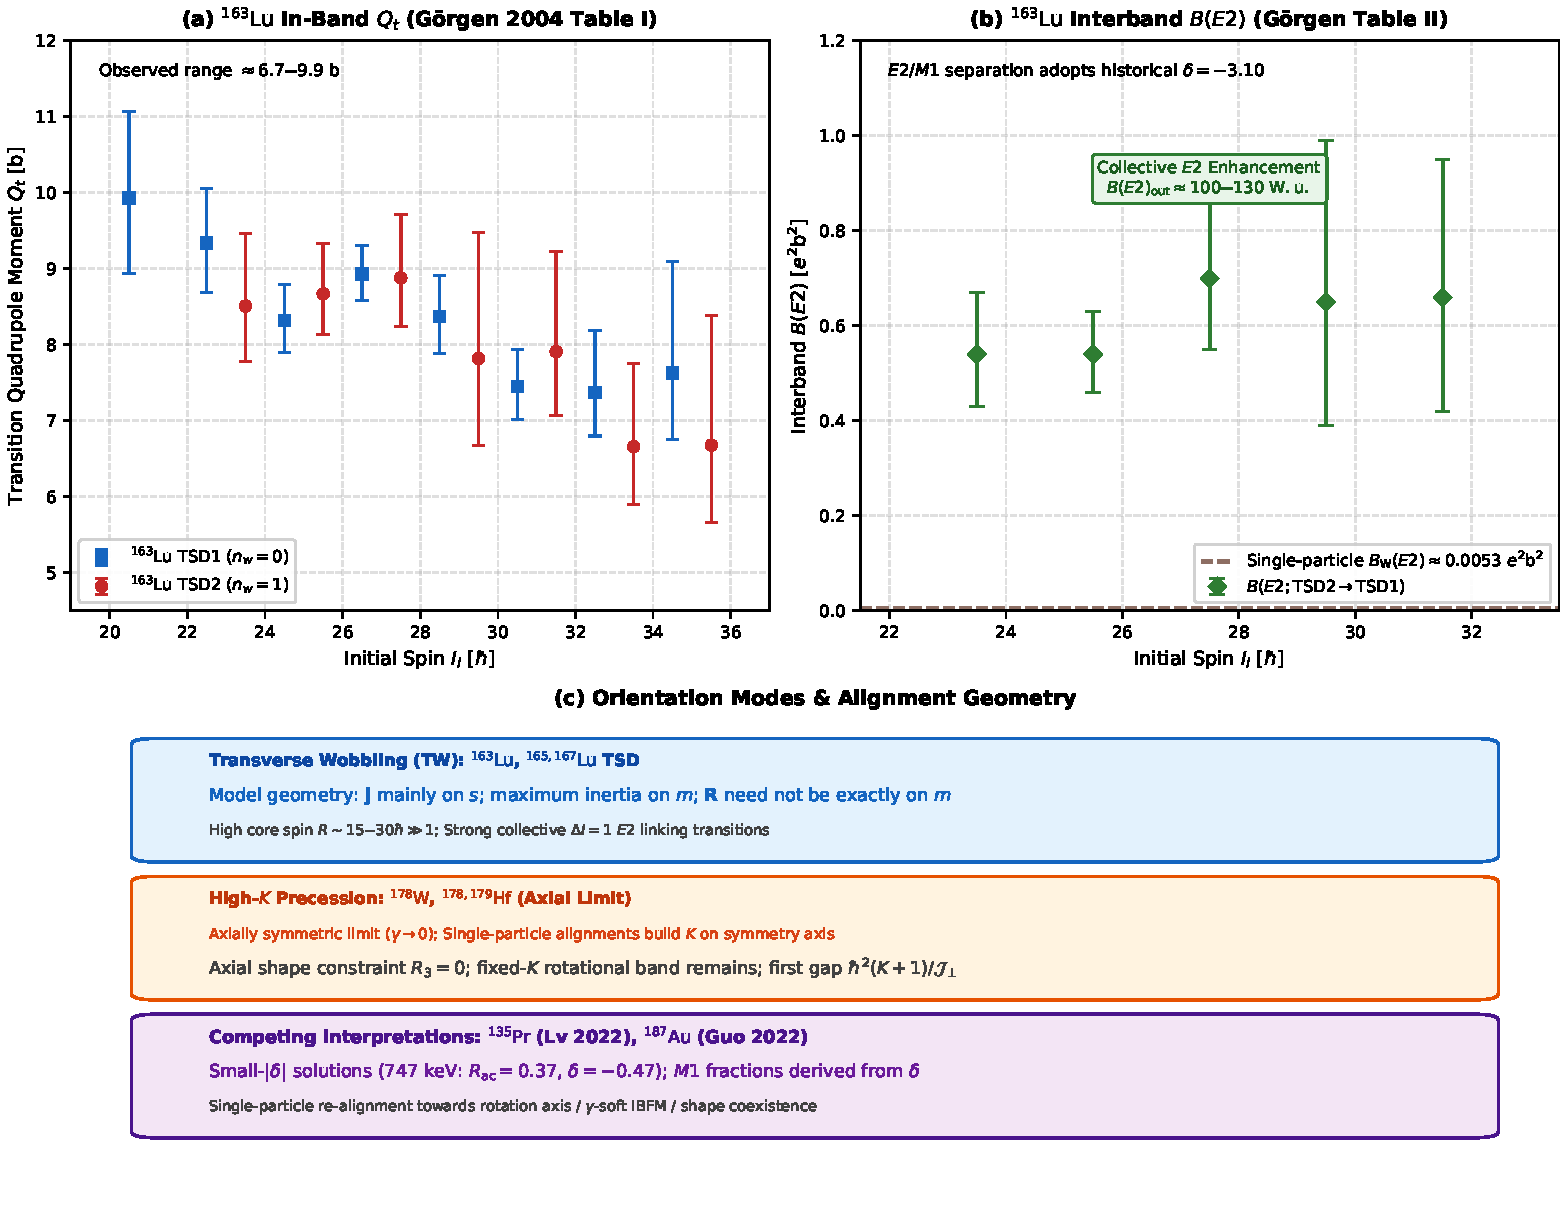
\includegraphics[width=\textwidth]{Img/orientation-comparison-modes.pdf}
\caption[跨核区典型非轴对称取向动力学模式对比：(a) $^{163}\mathrm{Lu}$ 带内跃迁四极矩 $Q_t$ 实测数据分布]{跨核区典型非轴对称取向动力学模式对比：(a) $^{163}\mathrm{Lu}$ 带内跃迁四极矩 $Q_t$ 实测数据分布（取自 Görgen 2004 Table I）；(b) $^{163}\mathrm{Lu}$ TSD2 向 TSD1 带间连接跃迁 $B(E2)$ 强度及集体增强判定（取自 Görgen 2004 Table II）；(c) 横向摆动（TW）、轴对称高 $K$ 进动以及平面转动/重对准三类典型取向模式的几何与角动量配置示意图。}\label{fig:4-4-orientation-modes}
\end{figure}

\subsection{取向自由度、主轴惯量排序与准粒子对准几何}\label{sec:4-4-1}

为了在同一物理约定下跨越不同质量区比较取向运动，首先必须严格厘清电荷空间几何主轴与转动惯量主轴的物理分离，显式给出几何坐标与动力学展开坐标的映射关系，并从微观壳层驱动力出发明确准粒子取向的对准机制。

\subsubsection{电荷几何主轴与转动惯量主轴的物理分离}

在内禀参考系中，非轴对称变形核的电荷表面在小形变近似展开下由形变参数 $\beta_2$ 与三轴不对称角 $\gamma$ 描述。沿用本稿显式给出的正 $\gamma$ 扇区及轴编号，空间电荷几何半径在小形变下为：
\begin{equation}\label{eq:4-4-radii-def}
R_k = R_0 \left[ 1 + \sqrt{\frac{5}{4\pi}}\beta_2 \cos\left(\gamma - \frac{2\pi}{3} k\right) \right], \qquad k = 1, 2, 3.
\end{equation}
为了严格确定三个几何主轴的相对尺度，令无量纲形变因子 $a \equiv \sqrt{\frac{5}{4\pi}}\beta_2 > 0$。在标准三轴扇区 $0^\circ < \gamma < 60^\circ$ 内，逐一考察式~\eqref{eq:4-4-radii-def} 中的余弦因子：
\begin{itemize}
\item 对于 $k=1$：$\cos\left(\gamma - \frac{2\pi}{3}\right) = \cos\left(120^\circ - \gamma\right)$。由于 $0^\circ < \gamma < 60^\circ$，其自变量满足 $60^\circ < 120^\circ - \gamma < 120^\circ$，因此 $\cos\left(\gamma - \frac{2\pi}{3}\right) \in \left(-\frac{1}{2}, \frac{1}{2}\right)$；
\item 对于 $k=2$：$\cos\left(\gamma - \frac{4\pi}{3}\right) = \cos\left(240^\circ - \gamma\right) = \cos\left(120^\circ + \gamma\right)$。其自变量满足 $120^\circ < 120^\circ + \gamma < 180^\circ$，因此该因子在全扇区恒取负值且满足 $\cos\left(\gamma - \frac{4\pi}{3}\right) \in \left(-1, -\frac{1}{2}\right)$；
\item 对于 $k=3$：$\cos\left(\gamma - 2\pi\right) = \cos\gamma$。其自变量满足 $0^\circ < \gamma < 60^\circ$，该因子恒取正值且满足 $\cos\gamma \in \left(\frac{1}{2}, 1\right)$。
\end{itemize}
比较上述三个区间的取值，可知在整个标准三轴扇区 $0^\circ < \gamma < 60^\circ$ 内，三角因子严格满足单调偏序：
\begin{equation}\label{eq:4-4-cos-order}
\cos\left(\gamma - \frac{4\pi}{3}\right) < \cos\left(\gamma - \frac{2\pi}{3}\right) < \cos\gamma.
\end{equation}
将式~\eqref{eq:4-4-cos-order} 代回半径定义式~\eqref{eq:4-4-radii-def}，直接导出核物质几何半径的大小排序：
\begin{equation}\label{eq:4-4-radii-order}
R_2 < R_1 < R_3.
\end{equation}
式~\eqref{eq:4-4-radii-order} 表明：在式~\eqref{eq:4-4-radii-def} 的轴编号下，几何主轴的对应关系为：
\begin{equation}\label{eq:4-4-axes-identity}
\begin{aligned}
\text{最短几何轴 (short, $s$ 轴)} &\iff k = 2; \\
\text{中间几何轴 (intermediate, $m$ 轴)} &\iff k = 1; \\
\text{最长几何轴 (long, $l$ 轴)} &\iff k = 3.
\end{aligned}
\end{equation}
在轴对称长椭极限 $\gamma \to 0^\circ$ 处，$\cos(-120^\circ) = \cos(-240^\circ) = -1/2$，导出 $R_1 = R_2 = R_0(1 - a/2) < R_3 = R_0(1+a)$（3轴为长椭旋转对称轴）；而在轴对称扁椭极限 $\gamma \to 60^\circ$ 处，$\cos(-60^\circ) = \cos(60^\circ) = 1/2$，$\cos(-180^\circ) = -1$，导出 $R_2 = R_0(1-a) < R_1 = R_3 = R_0(1+a/2)$（2轴为扁椭旋转对称轴）。这一逐式推导确立了主轴尺度几何关系，与第\ref{chap:2}章及第\ref{sec:3-2}节的主轴体系保持严格统一。

电荷几何半轴的大小排序，并不等同于核转动惯量张量的主轴排序。在核多体动力学中，转动惯量深刻受制于质量传输机制：
\begin{enumerate}
\item \textbf{经典刚体转动惯量}：绕第 $k$ 主轴的刚体惯量由垂直于该轴的物质密度二阶矩决定，即 $\mathcal{J}_k^{\text{rig}} = \int \rho(\mathbf{r}) (r^2 - x_k^2) d^3r \propto R_i^2 + R_j^2$（$i \ne j \ne k$）。根据几何半径不等式~\eqref{eq:4-4-radii-order}，由两较大半轴决定的惯量最大，因此刚体模型预言：绕最短几何轴 $s$（$k=2$）的转动惯量最大，绕最长几何轴 $l$（$k=3$）的转动惯量最小：
\begin{equation}\label{eq:4-4-rigid-order}
\mathcal{J}_2^{\text{rig}} > \mathcal{J}_1^{\text{rig}} > \mathcal{J}_3^{\text{rig}} \iff \mathcal{J}_s^{\text{rig}} > \mathcal{J}_m^{\text{rig}} > \mathcal{J}_l^{\text{rig}}.
\end{equation}
\item \textbf{无旋流体转动惯量}：在玻尔无旋流体模型中，惯量表达式为 $\mathcal{J}_k^{\text{irr}} = 4 B \beta^2 \sin^2\left(\gamma - \frac{2\pi}{3} k\right)$。在 $\gamma = 30^\circ$ 处，$\sin^2(-90^\circ) = 1$（$k=1$），而 $\sin^2(150^\circ) = \sin^2(30^\circ) = 1/4$（$k=2, 3$）。无旋流模型预言：绕中间几何轴 $m$（$k=1$）的转动惯量最大：
\begin{equation}\label{eq:4-4-irrot-order}
\mathcal{J}_1^{\text{irr}} > \mathcal{J}_2^{\text{irr}}, \mathcal{J}_3^{\text{irr}} \iff \mathcal{J}_m^{\text{irr}} > \mathcal{J}_s^{\text{irr}}, \mathcal{J}_l^{\text{irr}}.
\end{equation}
当 $0^\circ < \gamma < 30^\circ$ 时，$\mathcal{J}_1 > \mathcal{J}_2 > \mathcal{J}_3$；在 $\gamma = 30^\circ$ 处 $\mathcal{J}_2 = \mathcal{J}_3$；当 $30^\circ < \gamma < 60^\circ$ 时则演化为 $\mathcal{J}_1 > \mathcal{J}_3 > \mathcal{J}_2$。
\item \textbf{微观动态惯量响应}：在真实原子核中，由于费米子单粒子结构与残余配对关联，有效惯量张量并不必然处于刚体与无旋流的静态包络内，而是可以表现出显著的自洽转动角频率依赖性 $\mathcal{J}_k(\omega)$（如第\ref{sec:2-6}节与第\ref{sec:3-3}节所述，Matsuzaki 等人 2004）~\cite{matsuzaki-2004-nuclear-inertia-and-wobbling}。
\end{enumerate}

\subsubsection{准粒子取向趋势、局部动力学坐标置换与横向/纵向摆动模型边界}

奇 $A$ 核与多准粒子激发态的取向运动，由未配对价准粒子的内禀角动量 $\mathbf{j}$ 与变形核芯集体角动量 $\mathbf{R}$ 的矢量相加 $\mathbf{I} = \mathbf{R} + \mathbf{j}$ 决定。在变形平均场中，单粒子轨道受到各向异性四极驱动势的作用：
\begin{itemize}
\item \textbf{粒子型准粒子（处于子壳层底部）}：
在所讨论的高 $j$ 单壳层四极场模型中，费米面靠近子壳层底部的粒子型准粒子，其角动量 $\mathbf{j}$ 通常倾向于\textbf{对准短几何轴（$s$ 轴，即 $k=2$ 轴）}，例如用于描述 $^{163}\mathrm{Lu}$ 的 $\pi i_{13/2}$ 组态。这是由单粒子四极能与占据所给出的模型趋势，不能仅由质量数或某一 $\Omega$ 标签推定真实转动态的对准方向；$^{187}\mathrm{Au}$ 的 $\pi h_{9/2}$ 对准问题正需要与其具体组态和惯量排序一起检验。
\item \textbf{空穴型准粒子（处于子壳层顶端）}：
在同一模型的空穴极限，四极场对组态能的作用相对于粒子情形改变，空穴角动量通常倾向于\textbf{对准长几何轴（$l$ 轴，即 $k=3$ 轴）}。这里的空穴描述是相对于满壳参考态的多体记账方式，不代表空穴受到一种额外的排斥势。
\item \textbf{半满壳准粒子}：
费米面处于壳层中段时，配对混合与三轴四极场可以使准粒子在中间几何轴（$m$ 轴，即 $k=1$ 轴）方向形成主要对准分量；这需要具体的单粒子或准粒子计算，不是半满壳普遍成立的选择定则。
\end{itemize}

在 Frauendorf 与 Dönau（2014）的粒子--转子模型（PRM）框架下，横向摆动（TW）与纵向摆动（LW）具有严格的几何定义~\cite{frauendorf-2014-transverse-wobbling}：
\begin{enumerate}
\item \textbf{横向摆动（TW）}：准粒子角动量 $\mathbf{j}$ 的优势取向垂直于核芯所具有的最大转动惯量轴。在典型的类无旋流排序下，最大惯量轴为中间轴 $m$（$k=1$），而粒子型准粒子主要沿短轴 $s$（$k=2$）对准。该定义比较的是这两个方向，不要求核芯角动量在所有自旋上恰好沿中轴。下文采用的冻结顺排低自旋分支，正是围绕总角动量沿短轴的定常解作小振幅展开；超过其稳定域后，需要重新求定常取向，不能沿用同一展开中心。
\item \textbf{纵向摆动（LW）}：准粒子角动量 $\mathbf{j}$ 与核芯最大转动惯量轴共线平行。若模型中核芯最大转动惯量依然沿中轴 $m$，则 LW 要求奇核子亦对准中轴。
\end{enumerate}

\textbf{坐标置换与第\ref{sec:3-3}节冻结顺排（FA）公式的精确映射}：
必须注意，式~\eqref{eq:4-4-axes-identity} 给出的电荷几何主轴指标为 $k_1 = m, k_2 = s, k_3 = l$；而第\ref{sec:3-3}节在推导冻结顺排（FA）小振幅频率时，采用的局部动力学指标约定为：局部轴 1 沿冻结顺排准粒子方向，局部轴 2 沿核芯最大转动惯量轴，局部轴 3 沿剩余横向轴。在所讨论的横向摆动（TW）情形中，准粒子对准几何短轴 $s$（$k=2$），核芯最大惯量在中轴 $m$（$k=1$）。为了避免数字下标混淆，我们显式采用几何主轴指标 $(s, m, l)$ 重写相应的动力学恢复力曲率与能谱参数。相应的转动常数定义为 $A_s = \frac{\hbar^2}{2\mathcal{J}_s}, A_m = \frac{\hbar^2}{2\mathcal{J}_m}, A_l = \frac{\hbar^2}{2\mathcal{J}_l}$。有效转动常数表示为：
\begin{equation}\label{eq:4-4-A-s-bar}
\bar{A}_s \equiv A_s \left( 1 - \frac{j}{I} \right).
\end{equation}
两个横向恢复力曲率分别沿中轴 $m$ 与长轴 $l$ 展开：
\begin{equation}\label{eq:4-4-curvatures-sml}
C_m = (A_m - A_s) + A_s \frac{j}{I}, \qquad C_l = (A_l - A_s) + A_s \frac{j}{I}.
\end{equation}
定义曲率差参数 $a_m \equiv A_m - A_s$ 与 $a_l \equiv A_l - A_s$。在类无旋流排序下，$\mathcal{J}_m > \mathcal{J}_s \ge \mathcal{J}_l \implies A_m < A_s \le A_l$，因此 $a_m < 0$ 而 $a_l \ge 0$。小振幅简谐摆动激发频率表示为：
\begin{equation}\label{eq:4-4-wob-freq-sml}
\hbar\omega_{\text{wob}} = 2I\sqrt{C_m C_l} = 2\sqrt{\left( a_m I + A_s j \right) \left( a_l I + A_s j \right)}.
\end{equation}
相应的临界分叉自旋为中轴曲率 $C_m(I_c) = 0$ 处：
\begin{equation}\label{eq:4-4-critical-spin-sml}
I_c = \frac{j}{1 - A_m / A_s} = \frac{j}{1 - \mathcal{J}_s / \mathcal{J}_m}.
\end{equation}

\textbf{微观机制与理论边界辨析}：必须强调第\ref{sec:3-2}、\ref{sec:3-3}与\ref{sec:3-6}节建立的物理约束：
\begin{itemize}
\item \textbf{摆动能量的非单调性演化}：在式~\eqref{eq:4-4-wob-freq-sml} 中，由于 $a_m < 0$ 而 $a_l \ge 0$，因子 $(a_m I + A_s j)$ 随自旋线性下降，而因子 $(a_l I + A_s j)$ 随自旋线性上升。在低自旋区间，两因子的乘积完全可能呈现\textbf{先上升后下降}的非单调演化。因此，实验上测得有效摆动能量随自旋下降，仅能作为支持横向对准模型的条件性线索，绝对不能作为判定 TW 成立的排他性充要条件；反之，若在特定自旋段观察到能量轻微上升，亦不能据此单方面否定摆动机制。
\item \textbf{能量极小与线性动力学稳定性的区别}：在转动坐标系哈密顿体系中，若两个横向二次系数同时为正（$C_m > 0$ 且 $C_l > 0$），参考态处于定域能量曲面的严格极小值点，小振幅微扰构成良定义的正能声子激发基态。若 $C_m < 0$ 且 $C_l < 0$，乘积 $C_m C_l > 0$ 虽在形式上给出实数频率特征值，且该处作为能量极大值点在陀螺科里奥利力作用下可具备线性动力学稳定性（类似于经典刚体绕最小惯量轴转动在能量极大处依然保持线性稳定，见第\ref{sec:3-2}节的转子稳定性分析），但在物理上它对应能量曲面的极大，不能作为低能集体声子激发的稳定真空。
\item \textbf{临界分叉自旋 $I_c$ 的适用范围}：式~\eqref{eq:4-4-critical-spin-sml} 导出的 $I_c$ 严格依赖于准粒子角动量刚性冻结为 $j$ 的强定域近似以及特定的常数惯量排序。在真实原子核中，随着转动频率增加，科里奥利力迫使准粒子偏离短轴向旋转轴倾斜，有效对准投影发生动态演化，不能把常数 $I_c$ 当作全微观体系的严格相变点。
\item \textbf{倾斜转动（Tilt）不自动蕴含空间手征性破缺}：角动量矢量偏离主惯量转轴并发生倾斜（Tilted Axis Rotation），并不等价于手征对称性破缺。若总角动量矢量的倾斜轨迹完全局限在三个几何主平面之一（例如 $s-m$ 平面或 $l-m$ 平面内的平面倾斜），系统对特定主轴反演与时间反演的复合操作 $\mathcal{T}\mathcal{R}_k(\pi)$ 依然保持对称，体系不具备手征性；只有当角动量在三个主轴上同时具备非零分量、使相关的时间反演与半周转动复合对称性在内禀定常解中失效时，才具备所讨论模型的非平面手征几何条件（详见第\ref{sec:3-5}节与第\ref{sec:4-5}节）。
\end{itemize}

\subsection{经典三轴超形变摆动基准：$^{163}\mathrm{Lu}$ 的实测数据分析}\label{sec:4-4-2}

稀土区奇 $A$ 核素 $^{163}\mathrm{Lu}$（以及同位素 $^{165,167}\mathrm{Lu}$）的三轴超形变带（Triaxial Superdeformed, TSD），是核物理实验中多角度符合测量数据较为完备的摆动运动参照基准~\cite{odegard-2001-evidence-wobbling-163lu,jensen-2002-second-phonon-wobbling-163lu,campaign-g07-gorgen-2004-163lu-quadrupole-moments}。

\subsubsection{Görgen 2004 实验原表与跃迁强度数据}

Görgen 等人（2004）在劳伦斯伯克利国家实验室利用 Gammasphere 探测阵列，通过多普勒频移衰减法（DSAM）测量了 $^{163}\mathrm{Lu}$ TSD1 与 TSD2 能带的高自旋能级寿命与跃迁四极矩~\cite{campaign-g07-gorgen-2004-163lu-quadrupole-moments}。表~\ref{tab:4-4-lu163-sample}汇总了其论文 Table I 与 Table II 中所报告的代表性能级测量值、带内跃迁四极矩 $Q_t$ 以及带间连接跃迁的约化跃迁几率。

\begin{table}[!htbp]
\centering
\small
\caption{$^{163}\mathrm{Lu}$ 三轴超形变带能级寿命、带内 $Q_t$ 与带间连接跃迁强度（Görgen 2004 Tables I–II；$n_w$ 为摆动解释标签，派生强度保留所述分支与混合比输入）。}\label{tab:4-4-lu163-sample}
\begin{tabularx}{\textwidth}{p{2.2cm} p{2.0cm} c c c >{\raggedright\arraybackslash}X}
\hline\hline
\shortstack{能带与\\跃迁通道} & \shortstack{初态或\\跃迁自旋} & \shortstack{$E_\gamma$\\$\text{[keV]}$} & \shortstack{$\tau$\\$\text{[ps]}$} & \shortstack{$Q_t$\\$\text{[b]}$} & \shortstack{跃迁几率 / 强度\\$B(E2)$ 与 $B(M1)$} \\
\hline
\shortstack[l]{\textbf{TSD1}\\$(n_w=0)$} & $41/2^+$ & 578.6 & $0.364_{-0.085}^{+0.073}$ & $9.93_{-0.99}^{+1.14}$ & $B(E2) = 3.45_{-0.69}^{+0.80}\ e^2\mathrm{b}^2$ \\
带内 $\Delta I = 2$ & $45/2^+$ & 639.0 & $0.250_{-0.039}^{+0.035}$ & $9.34_{-0.65}^{+0.72}$ & $B(E2) = 3.07_{-0.43}^{+0.48}\ e^2\mathrm{b}^2$ \\
跃迁序列 & $49/2^+$ & 697.0 & $0.202_{-0.023}^{+0.021}$ & $8.32_{-0.42}^{+0.47}$ & $B(E2) = 2.45_{-0.25}^{+0.28}\ e^2\mathrm{b}^2$ \\
& $53/2^+$ & 752.6 & $0.119_{-0.010}^{+0.009}$ & $8.93_{-0.35}^{+0.38}$ & $B(E2) = 2.84_{-0.22}^{+0.24}\ e^2\mathrm{b}^2$ \\
& $57/2^+$ & 805.6 & $0.096_{-0.012}^{+0.011}$ & $8.37_{-0.49}^{+0.54}$ & $B(E2) = 2.50_{-0.29}^{+0.32}\ e^2\mathrm{b}^2$ \\
& $61/2^+$ & 857.7 & $0.088_{-0.011}^{+0.010}$ & $7.45_{-0.43}^{+0.49}$ & $B(E2) = 1.99_{-0.23}^{+0.26}\ e^2\mathrm{b}^2$ \\
& $65/2^+$ & 909.7 & $0.067_{-0.015}^{+0.010}$ & $7.37_{-0.57}^{+0.82}$ & $B(E2) = 1.95_{-0.30}^{+0.44}\ e^2\mathrm{b}^2$ \\
& $69/2^+$ & 962.5 & $0.047_{-0.011}^{+0.017}$ & $7.63_{-0.88}^{+1.46}$ & $B(E2) = 2.10_{-0.48}^{+0.80}\ e^2\mathrm{b}^2$ \\
\hline
\shortstack[l]{\textbf{TSD2}\\$(n_w=1)$} & $47/2^+$ & 654.6 & $0.215_{-0.048}^{+0.037}$ & $8.51_{-0.73}^{+0.95}$ & $B(E2) = 2.56_{-0.44}^{+0.57}\ e^2\mathrm{b}^2$ \\
带内 $\Delta I = 2$ & $51/2^+$ & 711.2 & $0.144_{-0.022}^{+0.017}$ & $8.67_{-0.53}^{+0.66}$ & $B(E2) = 2.67_{-0.33}^{+0.41}\ e^2\mathrm{b}^2$ \\
跃迁序列 & $55/2^+$ & 766.2 & $0.095_{-0.018}^{+0.013}$ & $8.88_{-0.64}^{+0.83}$ & $B(E2) = 2.81_{-0.41}^{+0.53}\ e^2\mathrm{b}^2$ \\
& $59/2^+$ & 819.9 & $0.087_{-0.037}^{+0.026}$ & $7.82_{-1.15}^{+1.66}$ & $B(E2) = 2.19_{-0.65}^{+0.94}\ e^2\mathrm{b}^2$ \\
& $63/2^+$ & 872.9 & $0.064_{-0.021}^{+0.013}$ & $7.91_{-0.84}^{+1.32}$ & $B(E2) = 2.25_{-0.48}^{+0.75}\ e^2\mathrm{b}^2$ \\
& $67/2^+$ & 926.5 & $0.075_{-0.025}^{+0.017}$ & $6.66_{-0.76}^{+1.09}$ & $B(E2) = 1.60_{-0.37}^{+0.52}\ e^2\mathrm{b}^2$ \\
& $71/2^+$ & 980.2 & $0.056_{-0.029}^{+0.017}$ & $6.68_{-1.02}^{+1.70}$ & $B(E2) = 1.61_{-0.49}^{+0.82}\ e^2\mathrm{b}^2$ \\
\hline
\textbf{TSD2} $\to$ \textbf{TSD1} & $47/2^+ \to 45/2^+$ & 658.9 & — & — & $B(E2) = 0.54_{-0.11}^{+0.13}\ e^2\mathrm{b}^2$, \\ & & & & & $B(M1) = 0.017_{-0.005}^{+0.006}\ \mu_N^2$ \\
带间 $\Delta I = 1$ & $51/2^+ \to 49/2^+$ & 673.2 & — & — & $B(E2) = 0.54_{-0.08}^{+0.09}\ e^2\mathrm{b}^2$, \\ & & & & & $B(M1) = 0.017_{-0.005}^{+0.005}\ \mu_N^2$ \\
连接跃迁 & $55/2^+ \to 53/2^+$ & 686.8 & — & — & $B(E2) = 0.70_{-0.15}^{+0.18}\ e^2\mathrm{b}^2$, \\ & & & & & $B(M1) = 0.024_{-0.007}^{+0.008}\ \mu_N^2$ \\
& $59/2^+ \to 57/2^+$ & 701.1 & — & — & $B(E2) = 0.65_{-0.26}^{+0.34}\ e^2\mathrm{b}^2$, \\ & & & & & $B(M1) = 0.023_{-0.011}^{+0.013}\ \mu_N^2$ \\
& $63/2^+ \to 61/2^+$ & 716.3 & — & — & $B(E2) = 0.66_{-0.24}^{+0.29}\ e^2\mathrm{b}^2$, \\ & & & & & $B(M1) = 0.024_{-0.010}^{+0.012}\ \mu_N^2$ \\
\hline\hline
\end{tabularx}
\end{table}

\subsubsection{实验数据特征、集体增强判定与客观证据边界}

核查 Görgen 等人（2004）的实测数据，可以提炼出 $^{163}\mathrm{Lu}$ 摆动运动解释的关键物理特征与严格的证据边界：
\begin{enumerate}
\item \textbf{四极形变的稳定性与微观一致性}：
TSD1 的跃迁四极矩在全测量自旋区间分布于 $7.37$--$9.93\ \mathrm{b}$（加权平均约为 $8.5\ \mathrm{b}$）；TSD2 的跃迁四极矩分布于 $6.66$--$8.88\ \mathrm{b}$（加权平均约为 $8.2\ \mathrm{b}$）。两带的 $Q_t$ 数值高度接近且随自旋演化行为一致，完全符合两能带建立在相近超形变核芯（推转计算给出 $\varepsilon_2 \approx 0.38, \gamma \approx +20^\circ$）之上的理论图像。必须说明，$n_w = 0, 1$ 属于作者的模型指派；相近的 $Q_t$ 是摆动模型的必要条件，但本身不足以单独排他性证明三轴刚性或多体波函数完全一致。
\item \textbf{带间连接跃迁的强烈电四极集体增强}：
连接 TSD2 与 TSD1 的 $\Delta I = 1$ 跃迁实测值高达 $B(E2)_{\mathrm{out}} = 0.54$--$0.70\ e^2\mathrm{b}^2$。采用标准核半径常数 $R_0 = 1.2 A^{1/3}\ \mathrm{fm}$，对于质量数 $A=163$，单个核子的标准 Weisskopf 单粒子估计为：
\begin{equation}\label{eq:4-4-weisskopf-e2}
B_{\mathrm{W}}(E2) = \frac{1}{4\pi}\left(\frac{3}{5}\right)^2 R_0^4 = 0.05940\, A^{4/3}\ e^2\mathrm{fm}^4 \approx 53.0\ e^2\mathrm{fm}^4 = 0.00530\ e^2\mathrm{b}^2.
\end{equation}
据此换算，实测带间跃迁几率 $0.54$--$0.70\ e^2\mathrm{b}^2$ 相当于高达约：
\begin{equation}\label{eq:4-4-lu163-wu}
B(E2)_{\mathrm{out}} \approx 100\text{--}132\ \mathrm{W.u.}
\end{equation}
的集体增强；而磁偶极跃迁强度约为 $B(M1) \approx 0.017$--$0.024\ \mu_N^2$。强烈的 $E2$ 集体增强与被压低的 $M1$ 强度，构成了带间跃迁由核芯宏观四极振动进动主导的关键实验证据。
\item \textbf{实验采用量依赖性与模型惯量边界}：
必须客观测定其方法学局限：在 Görgen 等人的分析中，从实测寿命中解离出 Table II 中的 $B(E2)$ 与 $B(M1)$，\textbf{依赖于前人在薄靶实验中测定的平均混合比 $\delta = -3.10_{-0.44}^{+0.36}$（Ødegård 2001，Jensen 2002）}~\cite{odegard-2001-evidence-wobbling-163lu,jensen-2002-second-phonon-wobbling-163lu}。该混合比在实验中仅测至自旋 $51/2^+$，更高自旋态的数值系假定该混合比保持不变外推提取所得。此外，理论文献中用于拟合 $^{163}\mathrm{Lu}$ 摆动能量的三个主轴转动惯量参数（如 $\mathcal{J}_m, \mathcal{J}_s, \mathcal{J}_l$）属于唯象拟合或微观推转/QRPA 模型的输出，绝不能将其误称作无模型依赖的实验直接实测量。
\item \textbf{自旋相空间与转动离心势}：
$^{163}\mathrm{Lu}$ 的两能带建立在很高的自旋区间（$I = 41/2^+$ 至 $71/2^+$）。在准粒子完全顺排估算下，核芯角动量算符模长估计达到：
\begin{equation}\label{eq:4-4-lu163-core-spin}
|\mathbf{R}| = |\mathbf{I} - \mathbf{j}| \sim (15\text{--}30)\hbar,\qquad R/\hbar\gg1.
\end{equation}
高速旋转产生的强离心势阱保证了集体转动维度的有效刚度，使得微扰进动波函数在谐振子极小附近高度局域化，从而使得局域谐振摆动近似在此处具备较高的物理适用度。
\end{enumerate}

\subsection{$A\approx 130$ 区域的低自旋摆动争议与极化双根仲裁}\label{sec:4-4-3}

当核物理学家试图将 $^{163}\mathrm{Lu}$ 的摆动图像向中重核区（$A\approx 130$）的低自旋带推广时，引发了近年来核结构领域关于角分布反演与微观竞争解释的深入学术讨论。

\subsubsection{Matta 等人（2015）的横向摆动宣称}

在奇质子核 $^{135}\mathrm{Pr}$（$Z=59, N=76$）中，奇质子占据侵入性的 $\pi 1h_{11/2}$ 轨道；TRS 势能面计算表明其基态具有中等三轴形变（$\beta_2 \approx 0.16, \gamma \approx 26^\circ$）。Matta 等人（2015）在阿贡国家实验室与印度 TIFR 利用 Gammasphere 与 INGA 阵列开展了在束测量，报道在负宇称基带（Band 1，自旋序列 $11/2^-, 15/2^-, 19/2^-, \dots$）旁观测到一条由 $\Delta I = 1$ 连接线相连的伴随带（Band 3，自旋序列 $13/2^-, 17/2^-, 21/2^-, \dots$）~\cite{matta-2015-transverse-wobbling-135pr}。作者宣称 Band 3 为基带之上的“一声子横向摆动带”，其主要依据包括：
\begin{enumerate}
\item 唯象摆动能量 $E_{\text{wob}}(I) \equiv E(I) - [E(I-1) + E(I+1)]/2$ 在低自旋区随自旋增加呈现下降趋势，符合 TW 简谐模型的唯象预期；
\item 对连接 Band 3 与 Band 1 的 $747.0\ \mathrm{keV}$ 等跃迁进行角分布拟合，提取出绝对值大于 1 的多极混合比解（如 $\delta = -2.0(4)$），对应电四极成分占比约为 $80\%$；
\item 测得这些特征连接跃迁的线偏振度不对称度呈现正值，据此推断这些跃迁具有电四极（$E2$）主导特征。
\end{enumerate}
随后，Sensharma 等人（2019）在同源的高统计量数字 Gammasphere（DGS）实验中进一步宣称观测到了 $^{135}\mathrm{Pr}$ 的“二声子横向摆动能带”~\cite{sensharma-2019-two-phonon-wobbling-135pr}。

\subsubsection{Lv 等人（2022）的独立实验再核查与角分布双根多义性}

郭松（S.~Guo）等人（2021）首先从方法学上指出了在束角分布拟合中固有的双根多义性问题~\cite{guo-2021-comment-transverse-wobbling-135pr}；随后，Lv 等人（2022）在芬兰于韦斯屈莱实验室利用 JUROGAM II 高分辨锗阵列完成了独立的高统计量符合重测，其结果对低自旋摆动声子图像提出了根本性的挑战~\cite{lv-2022-evidence-against-wobbling-135pr}：
\begin{enumerate}
\item \textbf{在束角分布拟合的二次有理式代数双根}：
在在束 $\gamma$ 谱学中，定向退激角分布函数展开为 $W(\theta) = 1 + A_2(\delta) P_2(\cos\theta) + A_4(\delta) P_4(\cos\theta)$，方向角关联比值 $R_{\mathrm{ac}}$ 同样由展开系数 $A_k$ 决定。根据第\ref{sec:5-9}节推导，展开系数 $A_k(\delta) = \frac{B_k + 2\delta C_k + \delta^2 D_k}{1 + \delta^2}$ 是关于多极混合比 $\delta$ 的二次有理式。因此，实验方程 $R_{\mathrm{ac}}^{\text{exp}} = R_{\mathrm{ac}}(\delta)$ 在整理后构成关于 $\delta$ 的一元二次方程。取决于实验比值与误差范围，方程在实数域内可具有两个实根、一个退化根或无有限实根。当存在两个实根时，通常表现为：
\begin{itemize}
\item 一个绝对值较大（$|\delta_1| > 1$），对应电四极主导（$E2$-rich）；
\item 另一个绝对值较小（$|\delta_2| < 1$），对应磁偶极主导（$M1$-rich）。
\end{itemize}
\item \textbf{线偏振符号与小根的相容性}：
Guo 等人（2021）与 Lv 等人（2022）明确指出：康普顿线偏振度不对称度 $P(\theta)$ 的数值与符号敏感依赖于初态自旋取向的统计分布张量以及混合比大小。在特定取向宽度与几何设置下，磁偶极主导的小根解同样可以给出正的线偏振度。因此，仅凭线偏振度呈现正符号，在物理上不能作为排他性支持大根、排除小根的充分证据。
\item \textbf{JUROGAM II 实测原表与能级分支比检验}：
严格核对能级跃迁与实测原表（Lv 等人 2022 Table 1）：
\begin{itemize}
\item 连接 Band 3 与 Band 1 的跃迁能量为 $747.3\ \mathrm{keV}$（其能级归属为 $17/2^- \to 15/2^-$）；实测线偏振度为 $P = 0.04_{-0.13}^{+0.08}$，角关联比值为 $R_{\mathrm{ac}} = 0.37(4)$，拟合出的小根解为：
\begin{equation}\label{eq:4-4-pr135-small-delta-747}
\delta = -0.47_{-0.22}^{+0.09}.
\end{equation}
在此小根解下，条件换算出的磁偶极辐射成分占比约为 $82\%$，电四极成分仅约 $18\%$；
\item 另一条关键连接线 $813.2\ \mathrm{keV}$（$21/2^- \to 19/2^-$），实测 $P = -0.03_{-0.12}^{+0.05}$，$R_{\mathrm{ac}} = 0.48(6)$，拟合出的小根解为：
\begin{equation}\label{eq:4-4-pr135-small-delta-813}
\delta = -0.37_{-0.14}^{+0.10},
\end{equation}
对应条件磁偶极成分占比约为 $88\%$；
\item 连接线 $450.2\ \mathrm{keV}$（$15/2^- \to 13/2^-$），实测 $R_{\mathrm{ac}} = 0.49(4)$，拟合出的小根解为 $\delta = -0.31_{-0.13}^{+0.10}$，对应条件磁偶极占比约为 $91\%$；
\item \textbf{同母态竞争分支比的检验}：从 Band 3 上的初态 $17/2^-$ 出发，存在两条平行的退激通道：落入基带 Band 1 的 $15/2^-$ 态（$747.3\ \mathrm{keV}$），以及落入签名伙伴带 Band 2 的 $13/2^-$ 态（$526.2\ \mathrm{keV}$）。Lv 等人在采用已测 $526.2\ \mathrm{keV}$ 多极性与相对强度后，导出约化四极跃迁几率之比为：
\begin{equation}\label{eq:4-4-pr135-branch-ratio}
\frac{B(E2; 747.3\ \mathrm{keV}, 17/2^- \to 15/2^-)}{B(E2; 526.2\ \mathrm{keV}, 17/2^- \to 13/2^-)} = 0.7_{-0.5}^{+0.7}.
\end{equation}
在纯横向摆动声子图像中，向基带的四极跃迁具有集体增强，向签名伙伴带的跃迁受到禁戒，上述比值在理论模型中通常预期显著大于 1。实测比值约为 0.7 表明初态波函数向两带具有同等量级的重叠，有力支持了能带混合的物理图像，向纯横向摆动声子模型提出了严重质疑。
\end{itemize}
\end{enumerate}

\subsubsection{微观多体竞争解释：IBFM、单粒子重对准与倾斜进动}

针对 $^{135}\mathrm{Pr}$ 的低自旋带，国际核结构理论界给出了多元竞争模型描述：
\begin{enumerate}
\item \textbf{微观相互作用玻色子-费米子模型（IBFM）}：
野村（K.~Nomura）等人（2022）基于相对论能量密度泛函 DD-PC1 与可分离配对力自洽映射偶偶核芯 $^{134}\mathrm{Ce}$ 的势能面，并拟合费米子--玻色子耦合参数，对 $^{135}\mathrm{Pr}$ 开展了微观 IBFM 计算（区分于该文中用于 $^{132}\mathrm{Ba} / ^{128}\mathrm{Xe}$ 的非相对论 Gogny D1M 泛函）~\cite{nomura-2022-questioning-wobbling-ibfm}。计算表明，$^{134}\mathrm{Ce}$ 核芯处于三轴 $\gamma$ 软势阱中。当奇质子与这一 $\gamma$ 软核芯发生四极动力学耦合时，自然形成了包含 Band 1 与 Band 3 的能级序列；模型理论预言两带间的连接跃迁天然由 $M1$ 主导，完全无须引入横向摆动激发假定。
\item \textbf{准粒子--三轴转子（QTR）放开冻结下的平面转动}：
Lv 等人（2022）利用固定三轴形变（$\varepsilon_2 = 0.16, \gamma = 26^\circ$）但放开准粒子取向自由度的微观 QTR 计算阐明：在带头自旋 $I = 13/2^-$ 处，扣除单粒子自旋 $j = 11/2\hbar$ 后，估算的核芯集体角动量仅为 $R = |\mathbf{I} - \mathbf{j}| \sim 1\hbar$ 左右。在弱转动离心势下，真实的量子角动量波函数在三维空间具有宽广的角向弥散，不能直接套用大自旋局域简谐高斯波包。随着自旋增加，奇核子角动量并非刚性冻结在短轴上，而是在科里奥利力作用下向主转动轴倾斜，发生单粒子对准重整（Planar Rotation），从而构成平面转动带。
\item \textbf{倾斜进动（Tilted Precession, TiP）模型}：
Lawrie 等人（2020）指出，在低自旋奇 $A$ 核中，体系角动量可能处于非主轴的经典倾斜平衡极小，表现为绕某一固定倾斜方向的准经典进动（TiP）~\cite{lawrie-2020-tilted-precession-wobbling}。这表明该核区实验数据存在多种相容的理论解读。
\end{enumerate}

\subsection{$A\approx 180$--$190$ 邻区：高 $K$ 进动极限与重区形状共存的取向演化}\label{sec:4-4-4}

迈向更重的超铪/钨（$A\approx 178$ 邻区）以及金/铂/汞（$A\approx 187$--$196$）过渡区时，非轴对称取向动力学展现出两类不同的物理边界：轴对称退化下的高 $K$ 进动几何，以及微观软势能面下的多重形状共存。

\subsubsection{高 $K$ 进动模式：三轴摆动的轴对称退化极限（Shimizu 2005）}

清水（Y.~R.~Shimizu）、松崎（M.~Matsuzaki）与松柳（K.~Matsuyanagi）（2005）利用微观随机相位近似（RPA）理论，探讨了高 $K$ 轴对称转动态与三轴摆动运动之间的几何联系~\cite{shimizu-2005-high-k-precession}。在 $^{178}\mathrm{W}$（如 $K^\pi = 25^+$）与 $^{178,179}\mathrm{Hf}$ 等长椭形变核中，多个破对费米子在轴对称变形场下发生取向叠加，在对称轴（取为 3 轴）上构筑起单粒子角动量无量纲投影 $K = \sum_i \Omega_i$。

考察三轴转子在 $\gamma \to 0^\circ$ 轴对称极限下的连续退化行为：
\begin{enumerate}
\item \textbf{参考系频率关系与无量纲量子数}：
在轴对称小振幅 RPA 展开下，对于物理 $\Delta K = +1$ 的进动激发模，实验室参考系进动角频率 $\omega_{\mathrm{prec}}$ 与均匀推转随体参考系转动角频率 $\omega_{\mathrm{rot}}$ 严格满足代数关系：
\begin{equation}\label{eq:4-4-shimizu-frame}
\omega_{\mathrm{wob}} = \omega_{\mathrm{prec}} - \omega_{\mathrm{rot}}, \qquad
\omega_{\mathrm{prec}} = \frac{\hbar K}{\mathcal{J}_\perp^{\text{eff}}(\omega_{\mathrm{prec}})}.
\end{equation}
式中无量纲量子数 $K \equiv \langle\Phi|J_3|\Phi\rangle/\hbar$ 为对称轴上的纯单粒子投影；垂直有效惯量 $\mathcal{J}_\perp^{\text{eff}}$ 一般依赖于进动模式频率，需自洽求解。
\item \textbf{对称轴冗余约束与能谱结构}：
对理想的轴对称形状转子，绕其对称轴（3 轴）的形状取向属于冗余坐标；模型以约束 $R_3 = 0$ 表达不存在独立的轴向集体形状转动。这并不意味着轴对称体系的微观推转响应在所有通道上恒为零。在保持固定内禀单粒子投影 $K$ 的绝热强耦合极限下，转动态仍具有垂直方向的集体转动，其能谱表达式为：
\begin{equation}\label{eq:4-4-high-k-energy-formula}
E_K(I) - E_{\text{intr}} = \frac{\hbar^2}{2\mathcal{J}_\perp} \left[ I(I+1) - K^2 \right], \qquad I = K, K+1, K+2, \dots
\end{equation}
\item \textbf{能级首间距与大 $K$ 进动领先项的区别}：
必须严格区分两个能标：
\begin{itemize}
\item 实验室参考系下带头\textbf{首个能级间距}（$I=K+1$ 与 $I=K$ 之间的跃迁能量）严格为：
\begin{equation}\label{eq:4-4-first-gap}
\Delta E_{\text{first}} = E_K(K+1) - E_K(K) = \frac{\hbar^2(K+1)}{\mathcal{J}_\perp};
\end{equation}
\item 而式~\eqref{eq:4-4-shimizu-frame} 给出的大 $K$ 极限（$K \gg 1$）下的经典领先阶进动角频率能量为：
\begin{equation}\label{eq:4-4-asymptotic-prec}
\hbar\omega_{\mathrm{prec}} \simeq \frac{\hbar^2 K}{\mathcal{J}_\perp}.
\end{equation}
\end{itemize}
二者之间相差严格的量度微商项 $\hbar^2/\mathcal{J}_\perp$，相对修正为 $1/K$。该代数关系反映了离散量子自旋与半经典进动之间的精确对应。
\end{enumerate}

\subsubsection{重区 $^{187}\mathrm{Au}$ 的实验检验与争议（Guo 2022）}

在奇 $A$ 重核过渡区核素 $^{187}\mathrm{Au}$（$Z=79$）中，围绕所谓的“纵向摆动（LW）”同样展开了学术论争。Sensharma 等人（2020）利用 Gammasphere 实验宣称在 $^{187}\mathrm{Au}$ 中基于奇质子 $1h_{9/2}$ 轨道观测到了纵向摆动能带（Band 2，带头自旋 $11/2^-$）~\cite{sensharma-2020-longitudinal-wobbling-187au}。

然而，郭松（S.~Guo）等人（2022）在兰州 HIRFL 加速器上开展了独立测量，结合微观分析指出该指派存在的物理争议~\cite{guo-2022-low-spin-wobbling-187au}：
\begin{enumerate}
\item \textbf{驱动势能与对准几何的倾向分歧}：
在 $^{187}\mathrm{Au}$ 中，质子数 $Z=79$，质子费米面靠近 $1h_{9/2}$ 子壳层的底部，属于粒子型准粒子。在微观势能面与四极场计算中，底壳粒子在能量上倾向于对准最短几何轴（$s$ 轴，即 $k=2$ 轴）。然而，Sensharma 等人的纵向摆动模型为了符合纵向摆动假定，将该准粒子角动量设定为对准中间几何轴（$m$ 轴，即 $k=1$ 轴），由此产生了对准几何的模型设定分歧。
\item \textbf{低自旋下的核芯转动动量估计}：
在 Band 2 带头 $I = 11/2^-$ 处，按顺排近似估计核芯集体角动量仅为 $R \sim 1\hbar$ 左右。在弱离心转动环境下，简谐微扰势阱的适用性受到挑战。
\item \textbf{角分布小根与采用强度的模型依赖性}：
Guo 等人通过电子内转换系数 $\alpha_K$ 测量以及角关联数据表明，连接 Band 2 与 Band 1 的特征跃迁 $376\ \mathrm{keV}$（$11/2^-$ $\to 9/2^-$）与 $462\ \mathrm{keV}$（$15/2^-$ $\to 13/2^-$）支持小混合比解（实验拟合给出 $\delta \approx -0.26$ 与 $-0.28$）。由于 $^{187}\mathrm{Au}$ 的 Band 2 能级寿命在比较数据集中缺乏直接测量，Guo 等人通过采用邻近偶偶核芯 $^{186}\mathrm{Pt}$ 的带内跃迁强度 $B(E2)_{\mathrm{in}} \sim 100$--$200\ \mathrm{W.u.}$ 进行折算，导出其实际带间跃迁强度较低：
\begin{equation}\label{eq:4-4-au187-be2-ratio}
\frac{B(E2)_{\mathrm{out}}}{B(E2)_{\mathrm{in}}} < 0.1, \qquad B(E2)_{\mathrm{out}} \sim \text{数个}\ \mathrm{W.u.}
\end{equation}
较低的带间电四极跃迁强度表明 Band 2 更自然地被解释为包含形状共存与单粒子态激发的多构型混合带。
\end{enumerate}

\subsubsection{重区 Os/Pt/Hg 的 $\gamma$ 软度与多重形状共存界限}

在重核过渡区（$^{186,188,190}\mathrm{Os}$、$^{188,190,192}\mathrm{Pt}$ 与 $^{190,192}\mathrm{Hg}$）的微观结构中，微观约束密度泛函（CDFT）与推转玻尔哈密顿量计算表明：部分核态势能面在 $\gamma$ 方向较为平缓，存在明显的 $\gamma$ 软振动与形状涨落，且普遍伴随能量相近的长椭与扁椭极小之间的多重形状共存（Shape Coexistence）~\cite{prochniak-rohozinski-2009-bohr-collective-hamiltonian}。

必须在此确立明确的物理分界：\textbf{绝对不能将该区域出现的弱四极形变或扁椭倾向，误认为是证实轴对称转子假设的依据；更不能将形状共存或软三轴核直接贴上刚性三轴摆动的排他性标签}。任何取向模式的判定，都必须结合能量曲面、微观轨道占据以及跃迁强度的综合测量。

\subsection{跨区迁移条件、物理不变量映射与失效反例}\label{sec:4-4-5}

通过对上述稀土区、中重区以及重核过渡区的系统对照，可以提炼出取向运动在原子核不同质量区发生迁移的物理条件，并明确微观不变量在实验表观量上的映射界限。

\subsubsection{取向运动跨区迁移的物理条件与失效机制}

一个具有三轴形变特征的原子核体系，若要在实验谱学中稳定呈现出宏观简谐摆动运动，通常需要满足以下综合物理条件：
\begin{enumerate}
\item \textbf{微观势能面刚度条件}：
核芯在内禀空间具备相对稳定的三轴形变势阱，避免被大振幅 $\gamma$ 软振动或多重形状共存所掩盖；
\item \textbf{集体转动离心势条件}：
体系总自旋显著超越未配对准粒子的内禀角动量，核芯分配到的集体转动动量较大（$R = |\mathbf{I} - \mathbf{j}| \gg 1$），从而构筑起简谐恢复力势阱；
\item \textbf{准粒子内禀对准稳定性}：
价核子费米面稳定处于高 $j$ 子壳层底部或顶端，且准粒子角动量在所研究的转动频率窗口内能够抵御科里奥利力引起的向转轴动态重对准；
\item \textbf{声子激发能隙解耦}：
摆动激发能量与局域两准粒子破对能、签名伙伴带交叉能级差以及核芯本身的 $\gamma$ 振动态保持足够的解耦间隙，以避免发生破坏声子特征的剧烈能带混合。
\end{enumerate}

低自旋候选核（如 $^{135}\mathrm{Pr}$ 与 $^{187}\mathrm{Au}$ 的低激发带）之所以难以呈现出典型摆动特征，其关键原因之一在于其违背了上述强转动假设：在带头处核芯转动极弱（$R \sim 1\hbar$ 左右），单粒子角动量极易受到推转诱导向主转轴发生重对准，导致体系在低自旋下更容易表现为由单粒子自旋翻转主导的平面转动或粒子--振动强耦合态。

\subsubsection{物理不变量与微观模型参数的映射边界}

在跨核区比较中，必须严格区分不同的微观或唯象物理量：
\begin{enumerate}
\item \textbf{跃迁四极矩 $Q_t$ 与光谱四极矩 $Q_s$}：$Q_t$ 由带内 $\Delta I = 2$ 跃迁寿命反演，反映的是电四极跃迁张量的非对角矩阵元大小；$Q_s$ 是核态本身的静态对角电四极矩。在非轴对称或形状涨落核中，相同的 $Q_t$ 不等价于两能带具有完全相同的微观多体波函数，更不能直接推导得出相同的转动惯量张量。
\item \textbf{克莱因不变量二次矩 $q_2$ 与三次矩 $q_3$}：在第\ref{sec:2-4}节中已经严格证明，通过库仑激发求和规则提取的形状不变量无量纲比值 $R \equiv q_3 / q_2^{3/2}$（正比于 $\langle Q^3 \cos 3\gamma \rangle$ $/ \langle Q^2 \rangle^{3/2}$），包含了体系在全部内禀形变空间中的大振幅积分权重。当核内存在强烈的 $\gamma$ 软振动时，$R$ 与刚体模型假定下的 $\cos 3\gamma$ 存在动力学偏差，不能简单建立一对一的代数换算。
\item \textbf{转动惯量的多重性}：由带内能级间距提取的运动学惯量 $\mathcal{J}^{(1)}$ 与动力学惯量 $\mathcal{J}^{(2)}$ 反映的是沿带的纵向转动响应；而决定摆动模式稳定性的是横向恢复力惯量 $\mathcal{J}_k(\omega)$。两者受控于截然不同的微观费米面与配对微商，不能用沿带间距直接推断横向动力学特征。
\item \textbf{电磁多极单位规范}：在磁偶极跃迁中，实验文献常用的传统原子核磁子单位 $\mu_N^2$ 与电荷型微观算符表述中的 $(\mu_N/c)^2$ 在标准定义下数值严格相同（如第\ref{sec:5-9}节式~\eqref{eq:5-9-delta-def} 所示），在任何换算中均不可人为施加多余的除以 $c^2$ 操作。
\end{enumerate}

\subsubsection{跨核区典型取向动力学对照总结}

表~\ref{tab:4-4-cross-region-comparison}汇总了跨越四大典型质量区的核态配置、形变机制、关键实测电磁可观测量以及当前理论界的主要竞争解释。

\begin{table}[!htbp]
\centering
\small
\caption{跨核区非轴对称取向动力学核心案例比较矩阵（上篇：微观构型、形变与惯量条件）。}\label{tab:4-4-cross-region-comparison-a}\label{tab:4-4-cross-region-comparison}
\begin{tabularx}{\textwidth}{p{2.6cm} p{5.5cm} >{\raggedright\arraybackslash}X}
\hline\hline
核素与能带标识 & 准粒子构型与费米面位置 & 形变与微观惯量模型条件 \\
\hline
$^{163}\mathrm{Lu}$ & 奇质子 $\pi i_{13/2}$；壳底粒子型对准短轴 $s=2$（模型假设 $\mathbf{j} \perp \mathcal{J}_m$） & $\varepsilon_2 \approx 0.38, \gamma \approx +20^\circ$；满足无旋流惯量主轴排序 $\mathcal{J}_m > \mathcal{J}_s > \mathcal{J}_l$ \\
TSD1 / TSD2 & & \\
\hline
$^{135}\mathrm{Pr}$ & 奇质子 $\pi 1h_{11/2}$；壳底粒子型，准粒子易受推转诱导重对准 & $\beta_2 \approx 0.16, \gamma \approx 26^\circ$；势能面具有中等三轴性，但微观配对导致惯量软化 \\
Band 1 / Band 3 & & \\
\hline
$^{178}\mathrm{W}$ & 多准粒子破对高 $K$ 态；费米子沿对称轴 $z=3$ 顺排形成宏观投影 $K = 25$ & 轴对称长椭极限 $\gamma \to 0^\circ$；形状冗余约束 $R_3 = 0$，垂直有效惯量 $\mathcal{J}_\perp^{\text{eff}}$ \\
$K^\pi = 25^+$ & & \\
\hline
$^{187}\mathrm{Au}$ & 奇质子 $\pi 1h_{9/2}$；壳底粒子型倾向短轴 $s=2$（与 LW 中轴对准假定分歧） & $\beta_2 \approx 0.15, \gamma \approx 18^\circ$；处于微观长椭--扁椭形状共存与 $\gamma$ 软振动区间 \\
Band 1 / Band 2 & & \\
\hline\hline
\end{tabularx}
\end{table}

\begin{table}[!htbp]
\centering
\small
\caption{跨核区非轴对称取向动力学核心案例比较矩阵（下篇：自旋窗口、实测特征与理论竞争）。}\label{tab:4-4-cross-region-comparison-b}
\begin{tabularx}{\textwidth}{p{2.1cm} p{3.0cm} p{4.3cm} >{\raggedright\arraybackslash}X}
\hline\hline
核素与能带 & 自旋窗口与带头转动 & 实测关键电磁特征 & 原作者解释 vs 主要竞争理论解释 \\
\hline
$^{163}\mathrm{Lu}$ & $I = 41/2^+$--$71/2^+$；模型估算 $R \sim 15$--$30\hbar \gg 1$（强离心势） & $Q_t \approx 6.7$--$9.9\ \mathrm{b}$；\newline 带间 $B(E2)_{\mathrm{out}} \approx 0.54$--$0.70\ e^2\mathrm{b}^2$（约 $100$--$132\ \mathrm{W.u.}$）；采用 $\delta \approx -3.10$ & 原作者：经典横向摆动 (TW)；\newline 理论评述：具备极强超形变势阱与高核芯离心转动的典型基准 \\
\hline
$^{135}\mathrm{Pr}$ & $I = 11/2^-$--$25/2^-$；带头自旋 $13/2^-$，估算 $R \sim 1\hbar$ 极微弱 & $747.3\ \mathrm{keV}$ 跃迁小根解 $\delta \approx -0.47$，$M1$ 成分占 $\sim 82\%$；$B(E2; 747)/B(E2; 526) \approx 0.7$ & 原作者 (Matta 2015)：低自旋 TW；\newline 竞争解释 (Lv 2022)：双根多义性，单粒子重对准平面转动 / IBFM / 能带混合 \\
\hline
$^{178}\mathrm{W}$ & $I \ge K = 25^+$；绕对称长轴进动，满足强耦合谱代数 & 带内强烈回转 $\Delta I = 1, 2$；首跃迁间距 $\frac{\hbar^2(K+1)}{\mathcal{J}_\perp}$；大 $K$ 渐近频率 $\hbar\omega_{\mathrm{prec}} \simeq \frac{\hbar^2 K}{\mathcal{J}_\perp}$ & 原作者 (Shimizu 2005)：高 $K$ 进动；\newline 物理联系：三轴摆动在轴对称下的连续几何演化极限 \\
\hline
$^{187}\mathrm{Au}$ & $I = 9/2^-$--$21/2^-$；带头自旋 $11/2^-$，估算 $R \sim 1\hbar$ 极微弱 & $376, 462\ \mathrm{keV}$ 跃迁小根解 $\delta \approx -0.26, -0.28$；采用 $^{186}\mathrm{Pt}$ 估计 $B(E2)_{\mathrm{out}}$ 仅数 W.u. & 原作者 (Sensharma 2020)：纵向摆动；\newline 竞争解释 (Guo 2022)：对准几何分歧，带头缺乏离心恢复力，多重形状共存 \\
\hline\hline
\end{tabularx}
\end{table}

综上所述，原子核在三轴形变空间中的动力学取向，绝非由单一的标量形变参数 $\gamma$ 所能片面确定，而是由核芯势能面曲率、微观费米面单粒子代数结构、集体转动惯量的自洽动力学响应以及自旋相空间所共同决定的复杂多体过程。在跨核区谱学研究中，唯有坚持将实验二次有理双根的多义性检验、高精度绝对寿命测量以及放开冻结近似的微观多体模型紧密结合，才能在纷繁复杂的实验谱线与深层核结构机制之间建立起可证伪、可复现的科学联系。
%
}{%
    \section{$A\approx 130$、稀土与重区的取向对照 [未完成]}\label{sec:4-4}%
    \textit{本节尚未完成。}%
}

%-- Section 4.5: Br/As与其它核区的反射—手征问题
\setcounter{section}{4}%
\IfFileExists{Tex/Sections/sec-4-5.tex}{%
    \section{Br/As 与其它核区的反射---手征问题}\label{sec:4-5}

在奇奇核与奇 $A$ 核的高自旋谱学中，当实验能级纲图上同时呈现出两对具有相近能量序列的正负宇称能带、且正负宇称带之间观测到相互交织的电偶极 $E1$ 连接跃迁时，一个引人瞩目的科学问题随之产生：这些在实验室系中呈现相近能级间隔的状态，是否如早期文献所探讨的那样，属于内禀手征对称性与空间反射对称性同时发生自发破缺所形成的“手征---宇称四重简并带（Chiral-Reflection Quartet, CPQ）”？

在理想的理论几何图像中，若原子核具备稳定的三轴非对称核芯（使四极内禀密度不再轴对称）并同时具备非平面的三维角动量几何（打破手征对称性），同时具备稳定的梨形八极形变（打破空间反演对称性），在固定有向体轴且确有相关定域构型的理想图像中，可用手征左右与八极朝向标记四个内禀构型；是否形成四个独立投影低能态仍须检验。必须明确指出：三轴形变本身仅打破轴对称性，并不自动导致手征对称性破缺；手征对称性自发破缺严格要求价质子、价中子与三轴核芯集体转动角动量矢量在空间构成非平面的三维取向结构。此外，第\ref{sec:2-5}节建立的量子投影恢复原理以及第\ref{sec:3-5}节对手征几何的微观解构明确指出：内禀平均场波函数的对称性破缺并不等价于实验室体系中四条能带的严格简并。特别是在 $A \approx 80$ 过渡核区中，单粒子自由度、三轴柔顺性与微观形状涨落紧密交织。本节以山东大学刘晨等人（2016年）关于 $^{78}\mathrm{Br}$ 的实验工作与肖骁等人（2019/2022年）关于 $^{74}\mathrm{As}$ 的实验工作为主线，从第一手测量链与实际跃迁网络出发，系统辨析该核区的数据现状与理论解释，阐明当前实验数据尚不足以确立来自同一相关内禀构型空间的静态手征---宇称四重带，厘清实验室好宇称态与内禀反射不对称的本质区别，解离内禀电偶极矩 $D_0$ 的模型依赖性，并给出该前沿方向上可证伪的研究检验路径~\cite{liu-2016-octupole-correlations-multiple-chiral-doublet-bands-78br,liu-chen-2016-78br-chirality-reflection-symmetry-thesis,xiao-2022-chirality-octupole-correlations-74as,xiao-xiao-2019-high-spin-74as-thesis,butler-1996-octupole-shapes,wang-2019-rat-prm-78br-octupole-correlations}。

\subsection{可追溯的能带结构与实际测量载荷}\label{sec:4-5-1}

为了确保学术讨论完全建立在经过严格实验检验的客观事实之上，表~\ref{tab:4-5-bands-summary}汇总了 $^{78}\mathrm{Br}$ 与 $^{74}\mathrm{As}$ 在第一手在束实验中实际观测到的能带编号、自旋宇称范围、微观组态指派以及直接测得的特征跃迁参量。

\begin{table}[!htbp]
\centering
\footnotesize
\caption{$^{78}\mathrm{Br}$ 与 $^{74}\mathrm{As}$ 中相关能带的观测自旋范围、组态指派与实验测量载荷汇总（严格依据刘晨 2016 博士论文与 PRL 2016、肖骁 2019 硕士论文与 PRC 2022 原件核对）。}\label{tab:4-5-bands-summary}
\begin{tabularx}{\textwidth}{p{2.0cm}p{1.6cm}p{1.9cm}p{3.0cm}>{\raggedright\arraybackslash}X}
\hline\hline
核素与反应条件 & 能带标识 & 自旋宇称范围 & 微观组态指派 & 实测跃迁网络与客观测量边界 \\
\hline
$^{78}\mathrm{Br}$ & Band 1 ($\pi=+$) & $7^+$ 至 $(20^+)$（图1） & $\pi g_{9/2} \otimes \nu g_{9/2}$ & 带内 $E2$ 级联；通过 $\Delta I=1$ 跃迁接收 Band 2 馈送；由 8 条 $E1$ 跃迁与 Band 3 互连；所引工作未给相关带的绝对寿命 \\
\shortstack[l]{$^{70}\mathrm{Zn}$\\$(^{12}\mathrm{C}, p3n)$} & Band 2 ($\pi=+$) & $9^+$ 至 $13^+$（图1） & $\pi g_{9/2} \otimes \nu g_{9/2}$ & 测得 ADO 比值与线偏振度；与 Band 1 构成手征候选双带；在当前探测灵敏度下未测得连接至负宇称带的 $E1$ 跃迁 \\
60, 65 MeV & Band 3 ($\pi=-$) & $6^-$ 至 $(19^-)$（图1） & $\pi f_{5/2}(p_{3/2}) \otimes \nu g_{9/2}$ & 带内 $E2$ 级联；测得带间分支比 $B(E1)/B(E2)$；由 8 条 $E1$ 跃迁连接至 Band 1；所引工作未给相关带的绝对寿命 \\
iThemba AFRODITE & Band 4 ($\pi=-$) & $6^-$ 至 $(14^-)$（2016图1） & $\pi f_{5/2}(p_{3/2}) \otimes \nu g_{9/2}$ & 经 $404.3\ \mathrm{keV}$ 跃迁退激至 Band 3；与 Band 3 构成手征候选；在当前探测限度下未测得跨宇称 $E1$ 跃迁 \\
\hline
$^{74}\mathrm{As}$ & Band 1 ($\pi=+$) & $6^+$ 至 $(16^+)$（2022图1） & $\pi g_{9/2} \otimes \nu g_{9/2}$ & 带内 $E2$ 级联；与 Band 2 发生 $\Delta I=1$ 混合；由 3 条 $E1$ 跃迁接收 Band 3 馈送；所引工作未给相关带的绝对寿命 \\
\shortstack[l]{$^{74}\mathrm{Ge}$\\$(^4\mathrm{He}, 1p3n)$} & Band 2 ($\pi=+$) & $7^+$ 至 $(14^+)$（2022图1） & $\pi g_{9/2} \otimes \nu g_{9/2}$ & 测得 ADO 比值；$B(M1)/B(E2)$ 呈现奇偶交错；与 Band 1 构成手征双带；未见跨宇称连接 \\
58.6, 62.6 MeV & Band 3 ($\pi=-$) & 图1包含 $5^-,6^-$ 低端态，延伸至 $14^-$ & $\pi(f_{5/2}/p_{3/2}) \otimes \nu g_{9/2}$ & 带内 $E2$ 级联；由 $372.4, 919.4, 1293.4\ \mathrm{keV}$ 共 3 条 $E1$ 跃迁连接至 Band 1；所引工作未给相关带的绝对寿命 \\
iThemba AFRODITE & Band 4 ($\pi=-$) & 2019论文的负宇称序列；未与2022逐线映射 & 2019 学位报告候选带 & 2019 硕士论文纲图观测并指认（判定不满足手征判据，归为候选赝自旋伙伴带）；2022 期刊聚焦 1--3 带 \\
\hline\hline
\end{tabularx}
\end{table}

\textbf{实验谱系与数据源依赖性声明}：
必须明确澄清实验数据的谱系归属：刘晨博士论文中所比较的 $^{78}\mathrm{Br}$ 谱学部分与期刊 PRL 论文（Liu et al. 2016）同属在南非 iThemba LABS 利用 AFRODITE 高分辨锗探测阵列与 DIAMANT 带电粒子阵列开展的 $^{70}\mathrm{Zn}(^{12}\mathrm{C}, p3n)^{78}\mathrm{Br}$ 反应在束测量数据；肖骁硕士论文（2019年）与期刊 PRC 论文（Xiao et al. 2022）的相关测量同属在 iThemba LABS 利用 AFRODITE 阵列开展的 $^{74}\mathrm{Ge}(^4\mathrm{He}, 1p3n)^{74}\mathrm{As}$ 反应实验谱系。同一实验谱系的学位论文与期刊不能计作独立重复实验。不过，两版报告不必使用完全相同的事件选择或矩阵：2019论文约 $6.17\times10^9$ 与2022期刊约 $1.9\times10^9$ 的符合计数具有不同报告口径，尚没有共同门条件证明二者相同；刻度、子集与带号也应分别核对。

特别需要指出，对于 $^{74}\mathrm{As}$ 的负宇称能带结构，学术界存在不同的文献呈现版本：肖骁在其 2019 年硕士学位论文中构建了包含 thesis Band 4的完整能级纲图，并通过细致的 $S(I)$ 与惯量计算，明确论证了 Band 3 与 Band 4 并不满足严格的手征双重带判据，进而将其提出为可能的赝自旋伙伴带；而在 2022 年发表的正式期刊论文中，作者团队为了突出手征性与八极关联，集中报道了满足手征判据的正宇称双重带（Bands 1--2）以及与之具有强 $E1$ 跃迁连接的负宇称带（Band 3），期刊的负宇称Band 3与thesis Bands 3/4尚未完成唯一的逐线对应，不能仅按相同数字合并。因此，必须客观记录两个版本各自的学术侧重与原始报告，绝对不能武断宣称“Band 4 从未在实验中被观测到”。

\subsection{实际观测宇称连接网络拓扑}\label{sec:4-5-2}

根据原件测量数据绘制的能带连接网络如图~\ref{fig:4-5-network}所示。仔细审视实际跃迁网络的拓扑连接，有助于准确把握文献中关于“四重带”讨论的物理本质。

\begin{figure}[!htbp]
\centering
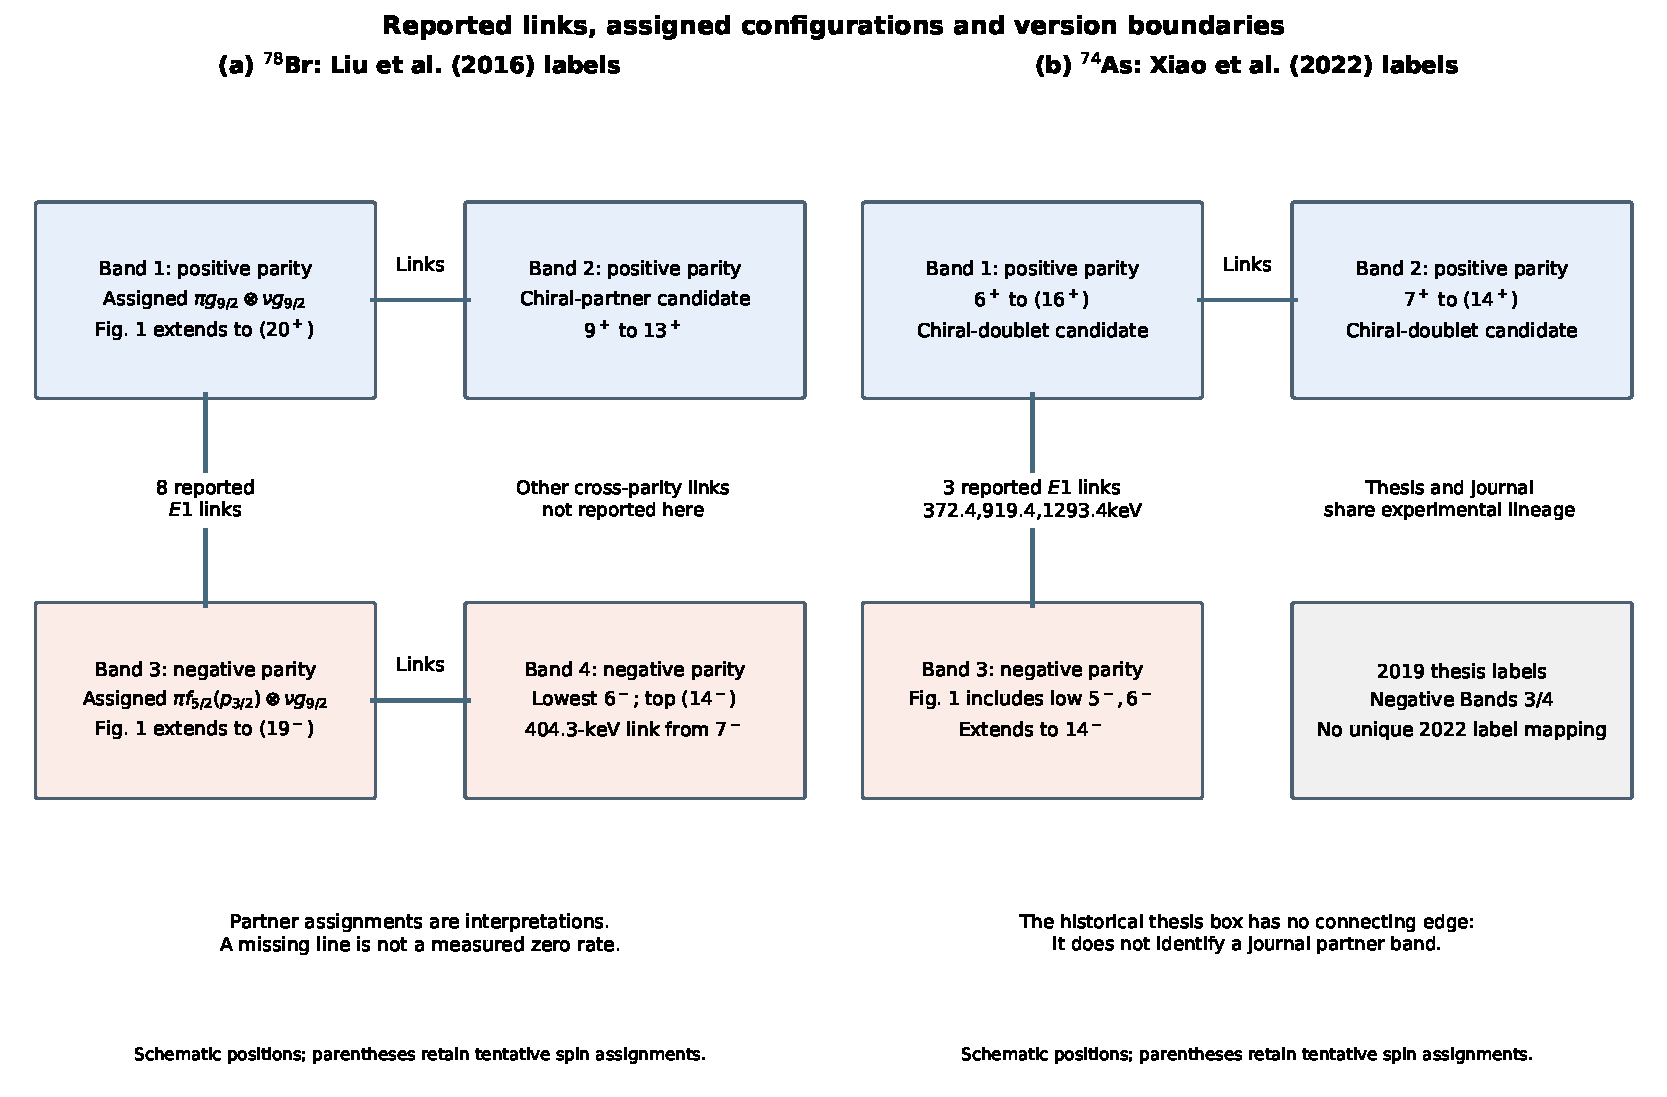
\includegraphics[width=0.88\textwidth]{Img/br-as-network-topology.pdf}
\caption[$^{78}\mathrm{Br}$ 与 $^{74}\mathrm{As}$ 实验中实际观测到的能带结构与跃迁连接网络拓扑示意图]{$^{78}\mathrm{Br}$ 与 $^{74}\mathrm{As}$ 实验中实际观测到的能带结构与跃迁连接网络拓扑示意图（依据 Liu et al. PRL 2016、刘晨 2016 博士论文、Xiao et al. PRC 2022 及肖骁 2019 硕士论文绘制；代码与数据来源见附录\ref{app:reproducible-inputs}）。(a) $^{78}\mathrm{Br}$ 中观测到的 4 条主带：正宇称带 Band 1, 2 与负宇称带 Band 3, 4 建立在不同的微观单粒子组态之上；8 条报告的 $E1$ 跃迁连接 Band 1 与 Band 3；图中连线只归纳带间联系，不表示一条光子跃迁具有双向发射率。其他连接未报告，所引资料未给统一数值上限；(b) $^{74}\mathrm{As}$ 中观测到的能带关联：正宇称双重带 Band 1, 2 与负宇称带 Band 3 通过 3 条实测 $E1$ 跃迁（$372.4, 919.4, 1293.4\ \mathrm{keV}$）互连；2019学位论文另有其负宇称Bands 3/4及候选赝自旋解释，未与2022负宇称带建立唯一逐线映射。}\label{fig:4-5-network}
\end{figure}

从图~\ref{fig:4-5-network}展示的真实网络拓扑中，可以得出两点明确的物理结论：
\begin{enumerate}
\item \textbf{$^{78}\mathrm{Br}$ 中的“多手征带伴随八极关联”与同构型静态四重带的区别}：
在 $^{78}\mathrm{Br}$ 中，正宇称能带（Band 1 与 Band 2）建立在 $\pi g_{9/2} \otimes \nu g_{9/2}$ 组态之上，由微观粒子--转子模型（TPRM）支持为一对正宇称手征双重带；而负宇称能带（Band 3 与 Band 4）建立在 $\pi f_{5/2}(p_{3/2}) \otimes \nu g_{9/2}$ 组态之上，被解释为另一对负宇称手征双重带。这两对能带在内禀组态上涉及不同的奇质子主导轨道占据。更关键的是，实验观测到的 8 条 $E1$ 连接跃迁局限在正宇称基带 Band 1 与负宇称带 Band 3 之间；在两个伴带 Band 2 与 Band 4 之间，以及 Band 2 与 Band 3、Band 1 与 Band 4 之间，在当前探测阵列统计限度内未测得明显的跨带 $E1$ 跃迁。需要指出，未见线需要结合效率、本底和统计选择才能量化为上限；所引资料未给出每条缺失连接的统一数值上限，不能据此置零；但作者将所见能带及模型比较解释为 $^{78}\mathrm{Br}$ 中基于所指派组态的多重手征双重带系统（Multiple Chiral Doublets, $M\chi D$）并伴随特定单侧能带间的八极关联，当前数据尚不足以确立在单一固定组态下由空间反射与手征同时破缺所构成的静态手征---宇称四重简并带。
\item \textbf{$^{74}\mathrm{As}$ 中缺乏闭合的四能带交织手征网络}：
在 $^{74}\mathrm{As}$ 中，2022 年期刊论文确立的强连接网络展现为 $2+1$ 的三能带结构：满足手征指纹的正宇称双重带（Band 1 与 Band 2）以及一条由 3 条 $E1$ 跃迁（$372.4, 919.4, 1293.4\ \mathrm{keV}$）连接的负宇称能带（Band 3）。即便在 2019 年学位论文包含了负宇称 Band 4 的原始纲图中，作者认为其负宇称Bands 3/4不满足所采用的手征判据，并保留赝自旋伙伴候选解释；这些是thesis自己的带号，不能把期刊E1网络倒赋给其中某一条。体系在现有实验精度下尚未展现出两对正负宇称手征双带对称交织构成的四重完全闭合网络。
\end{enumerate}

\subsection{理论概念桥梁：对称性、算符与几何误区}\label{sec:4-5-3}

面对上述实验拓扑，理论分析必须严格厘清不同离散对称性、量子力学算符以及表象之间的本质区别：

\subsubsection{实验室好宇称态与内禀反射不对称的区别}

在忽略弱相互作用宇称不守恒效应的核物理体系中，采用强相互作用与电磁相互作用哈密顿量 $\hat{H}$ 时，空间反演算符 $\hat{\mathcal{P}}$（$\mathbf{r} \to -\mathbf{r}$）与哈密顿量严格对易：
\begin{equation}\label{eq:4-5-parity-commute}
[\hat{H}, \hat{\mathcal{P}}] = 0.
\end{equation}
因此，在上述强与电磁哈密顿量下，体系的精确能量本征定态总可以选择为具有确定守恒空间宇称 $\pi = \pm 1$ 的好宇称态。文献中所讨论的“空间反射不对称性”，属于自洽平均场或内禀参考系近似下的物理图像。若微观平均场给出的能量极小态具备非零的内禀八极形变（$\beta_3 \neq 0$），则内禀波函数不具备确定的空间反射对称性：
\begin{equation}\label{eq:4-5-intrinsic-parity-breaking}
\hat{\mathcal{P}}\,|\Phi_{\mathrm{int}}(\beta_3)\rangle = |\Phi_{\mathrm{int}}(-\beta_3)\rangle \neq |\Phi_{\mathrm{int}}(\beta_3)\rangle .
\end{equation}
为了在实验室参考系中恢复精确守恒的角动量与空间宇称量子数，必须对内禀波函数执行严格的三维角动量与宇称联合投影。具有良好总角动量 $I$、实验室投影 $M$、确定宇称 $\pi$ 及能级指标 $\alpha$ 的物理态表示为：
\begin{equation}\label{eq:4-5-parity-projection}
|I M \pi; \alpha\rangle = \mathcal{N}_{I^\pi \alpha} \sum_K f_K^{I^\pi \alpha} \hat{P}_{MK}^I \left( \frac{1 + \pi \hat{\mathcal{P}}}{2} \right) |\Phi_{\mathrm{int}}\rangle ,
\end{equation}
这是所选有限投影试探空间中的构态方法，而非所有求解核态的方法都必须从该内禀态出发。其中 $\hat{P}_{MK}^I$ 为三维角动量投影算符，归一化因子 $\mathcal{N}_{I^\pi \alpha}$ 以及 $K$ 混合系数 $f_K^{I^\pi \alpha}$ 由该试探空间的角动量---宇称范数核、哈密顿核与广义本征问题确定；恢复量子数不保证变分空间已完备。单纯的宇称投影归一因子 $2(1 \pm \langle \Phi_{\mathrm{int}} | \hat{\mathcal{P}} | \Phi_{\mathrm{int}} \rangle)$ 仅适用于未投影角动量的一维情形，不能直接套用于包含三维欧拉角积分的复合投影态。

在一个存在两处反射相关定域构型的势阱模型中，量子混合可以使其宇称组合发生劈裂。只有同一 $I$ 的两种宇称态都存在且可作相关比较时，才定义同自旋位移：
\begin{equation}\label{eq:4-5-parity-gap}
\Delta E_{\text{parity}}(I) \equiv E^-(I) - E^+(I).
\end{equation}
转动能与形变相关惯量会改变八极有效势面，不能预设其对势垒高度总有同一作用。偶偶核的交替宇称序列还可能只在偶 $I$ 给出正宇称、奇 $I$ 给出负宇称；此时应采用后文相邻态插值的 $\delta E(I)$，不能虚构同 $I$ 的成对能级。无论何种位移，局域化、隧穿与组态混合都需在具体模型中判断。

\subsubsection{时间反演、手征操作与手征双重态}

为明确操作与内禀标签的关系，先取一个受限模型：四极张量在固定右手主轴 $(1,2,3)=(x,y,z)$ 上对角，且三个本征值互异；奇宇称形变仅含 $\beta_{30}Y_{30}$。这里的 $y=2$ 是明示坐标轴，不自动等于其他文献所叫的中间几何轴。下表均为对态与密度的\emph{主动}操作，并在同一组有向坐标轴上比较；电四极形状及电荷八极坐标均取时间反演偶。记 $\mathbf{a}=(a_1,a_2,a_3)$ 为 $\mathbf j_p,\mathbf j_n,\mathbf R$ 中任一轴角动量，定义
\begin{equation}\label{eq:4-5-chiral-op}
\mathcal C\equiv\mathcal T\mathcal R_y(\pi),\qquad
\mathcal D\equiv\hat{\mathcal P}\mathcal C.
\end{equation}
三矢量非共面的几何量是
\begin{equation}\label{eq:4-5-chiral-triple-product}
\chi=\mathbf j_p\cdot(\mathbf j_n\times\mathbf R)\ne0.
\end{equation}
其中各矢量可分别主要沿一个主轴，无需每个矢量的三个分量均非零。
\begin{center}
\begin{tabular}{c|c|c|c|c}
操作 & 四极张量 & $\beta_{30}$ & $\mathbf a$ & $\chi$ \\
\hline
$\hat{\mathcal P}$ & 不变 & $-\beta_{30}$ & $(a_1,a_2,a_3)$ & $+\chi$ \\
$\mathcal T$ & 不变 & $+\beta_{30}$ & $(-a_1,-a_2,-a_3)$ & $-\chi$ \\
$\mathcal R_y(\pi)$ & 不变 & $-\beta_{30}$ & $(-a_1,a_2,-a_3)$ & $+\chi$ \\
$\mathcal C$ & 不变 & $-\beta_{30}$ & $(a_1,-a_2,a_3)$ & $-\chi$ \\
$\mathcal D=\hat{\mathcal P}\mathcal C$ & 不变 & $+\beta_{30}$ & $(a_1,-a_2,a_3)$ & $-\chi$
\end{tabular}
\end{center}
此表本身不证明任意给定哈密顿量具有这些对称性；推转约束或其他时间反演奇场存在时还须核查实际哈密顿量。这里 $\chi$ 对空间反演为偶：三个角动量都是轴矢量，故不能把它误称为空间宇称奇量；它对时间反演为奇。若把主动旋转后的形状再通过体轴重标转回标准朝向，则必须同步变换角动量分量，不能只改写 $\beta_{30}$ 而保留原先的分量标签。$\beta_{30}$ 的符号是此处所选有向体轴中的朝向标签，亦不能与波函数受宇称作用所得的相位或实验室宇称本征值混同。

于是，以 $\eta=\pm$ 标记此坐标约定下的八极朝向、$L/R$ 标记 $\chi$ 的两种符号，可以选择态的相位，使对应关系在相位意义下写为
\[
\hat{\mathcal P}|L,\eta\rangle\sim|L,-\eta\rangle,\quad
\mathcal C|L,\eta\rangle\sim|R,-\eta\rangle,\quad
\mathcal D|L,\eta\rangle\sim|R,\eta\rangle.
\]
也就是说，本例中固定 $\eta$ 的左右手联系可由 $\mathcal D$ 实现，而第\ref{sec:3-7}节的标准 $\mathcal C$ 仍翻转手征符号；它们描述同一操作代数的不同组合。空间宇称与时间反演、旋转均对易，故 $[\hat{\mathcal P},\mathcal C]=0$。对整数或半整数总自旋 $I$，分别有 $\mathcal T^2=\mathcal R_y(\pi)^2=(-1)^{2I}$，从而 $\mathcal C^2=\mathcal D^2=+1$。$\mathcal C$ 与 $\mathcal D$ 均反幺正，态的重定相会改变其表观本征相位；$(1\pm\mathcal C)/2$ 不是复希尔伯特空间上的线性手征投影算符。相反，实验室良宇称由线性投影 $(1\pm\hat{\mathcal P})/2$ 分类。

\subsubsection{四重结构与模型边界}

上述表格只适用于指定的 $\beta_{30}$ 形状及坐标约定；一般八极张量的各分量在旋转下按三阶张量混合，不能一律赋予同一符号。Wang 等人的 RAT-PRM 另有核芯宇称、总宇称恢复和特定反射对称化，其基底与所选相互作用必须分别核查，不能将此表直接当成所有 RAT-PRM 的定义~\cite{wang-2019-rat-prm-78br-octupole-correlations}。即使四个对称相关内禀构型存在，也不能由标签数推出四个独立的投影低能态或四条近简并带：应检验角动量与宇称投影后的范数核秩、构型混合以及所保留的复合对称性，并考察相应哈密顿核。不同良宇称态具有不同主导轨道成分，也不能单凭这一点排除它们来自共同的反射不对称内禀态。

\subsubsection{符号区分：四极标量不变量 $q_3$ 与八极形变参数的区别}

在核张量代数与形变参数表述中，必须严格区分四极张量不变量与八极形变参量：
第\ref{sec:2-4}节定义的四极标量不变量 $q_3$ 为电四极算符 $\mathcal{M}(E2)$ 的三次完全收缩：
\begin{equation}\label{eq:4-5-q3-def}
q_3 \equiv -\sqrt{\frac{7}{2}}\,\langle (\mathcal{M}(E2) \times \mathcal{M}(E2))_2 \cdot \mathcal{M}(E2) \rangle .
\end{equation}
为了消除总体形变尺度的影响，采用无量纲矩比 $R=q_3/q_2^{3/2}$。按第1.2与2.4节相同的可交换集体坐标映射，它给 $\langle Q^3\cos3\gamma\rangle/\langle Q^2\rangle^{3/2}$；只有幅度和角度都足够局域时才近似单个 $\cos3\gamma$。由于 $q_3$ 还包含总体电四极幅度立方，未经 $q_2^{3/2}$ 归一化的 $q_3$ 不能作为独立的三轴不对称度指标；且 $q_3$ 在空间反演下具有偶宇称（$\hat{\mathcal{P}} q_3 \hat{\mathcal{P}}^{-1} = +q_3$）。

与之完全不同，描述原子核质荷分布反射不对称性的电八极形变参数 $\beta_3$ 是核表面径向展开参数，而电八极跃迁算符 $\mathcal{M}(E3)$ 具有电荷乘长度三次方量纲 $e\cdot\mathrm{fm}^3$（在空间反演下具有奇宇称，$\hat{\mathcal{P}} \mathcal{M}(E3) \hat{\mathcal{P}}^{-1} = -\mathcal{M}(E3)$）。二者不仅物理含义截然不同，数学量纲与变换性质亦完全不同，不可混同。

此外，微观约束自洽密度泛函（MDC-CDFT）或反射不对称三轴粒子--转子模型（RAT-PRM）计算给出的角动量有效夹角（如价质子、价中子与核芯转动角动量的有效夹角大于 $45^\circ$），属于特定截断模型空间与唯象参数下的计算结果，并不等同于实验直接测得经典角动量在空间的瞬时取向。

\subsection{竞争解释的强版本与 $E1$ 跃迁的物理机制}\label{sec:4-5-4}

理解正负宇称能带之间 $E1$ 连接跃迁的动力学机制，需要深入考察原子核电偶极辐射的微观与宏观机制。

\subsubsection{电偶极矩的微观与宏观机制}

在原子核中，质心运动在严格平移不变性下不产生电偶极辐射。在内禀坐标系中，$E1$ 辐射通过质子与中子电荷中心的相对分离产生：
\begin{enumerate}
\item \textbf{宏观质心--电荷中心再极化机制}：
在忽略质子与中子质量差的平移不变坐标中，沿内禀轴的电偶极矩可写为
\begin{equation}\label{eq:4-5-myers-dipole}
D_0=e\sum_{p}(z_p-R_{{\rm cm},z})
=e\frac{N}{A}\sum_p z_p-e\frac{Z}{A}\sum_n z_n.
\end{equation}
若质子与中子密度在各处按粒子数严格成比例，电荷中心与质量质心重合，即使密度有梨形分量也可有 $D_0=0$。实际偶极矩需考虑质中分布的相对极化、壳结构及相关效应；不能仅凭 $\beta_2\beta_3$ 的非零值指定一个跨核素普适的 $AZ$ 标度。
在剔除质心伪运动后，单质子与单中子的平移不变有效电偶极辐射电荷分别表示为：
\begin{equation}\label{eq:4-5-effective-charge}
e_{\text{eff}}^{\text{p}} = e \frac{N}{A}, \qquad e_{\text{eff}}^{\text{n}} = -e \frac{Z}{A}.
\end{equation}
\item \textbf{微观单粒子对的八极驱动机制}：
在微观壳模型中，产生强八极关联的关键在于费米面附近是否存在一对满足 $\Delta l = 3$ 且 $\Delta j = 3$、宇称相反的单粒子轨道对。必须强调：$\Delta l = \Delta j = 3$ 是轨道间产生大八极耦合矩阵元的有利微观驱动条件，而非电八极跃迁 $E3$ 的一般选择定则（$E3$ 跃迁至少须满足角动量三角不等式 $|j_i - j_f| \le 3 \le j_i + j_f$ 及宇称改变 $\Delta\pi=-$；允许性不保证矩阵元非零）。在 $A \approx 80$ 核区，质子侵入轨道 $1g_{9/2}$（$l=4, j=9/2$）与下层正常轨道 $2p_{3/2}$（$l=1, j=3/2$）满足该驱动条件。需要严格区分的是：负宇称带主导组态所涉及的 $\pi f_{5/2}$ 轨道虽然也参与近费米面相互作用，但它与 $g_{9/2} \leftrightarrow p_{3/2}$ 八极驱动轨道对具有不同的单粒子性质，不可将二者简单合并等同。
\end{enumerate}

\subsubsection{微观势能面软度与替代机制}

刘晨等人（2016）利用 PC-PK1 有效相互作用开展的微观约束多维协变密度泛函（MDC-CDFT）计算表明：其图6给出的 $^{78}\mathrm{Br}$ 势能面在 $\beta_{30}$ 方向较软，作者据此支持八极关联的解释；这不等于建立了所有相关构型的稳定非零八极极小。Wang 等人（2019）利用反射不对称三轴粒子--转子模型（RAT-PRM）计算时，采用固定的非零八极参数输入（如 $\beta_3=0.02$）考察反射不对称的影响；固定参数计算本身没有建立 $\beta_3$ 运动的完整动态涨落，计算表明负宇称带的电磁特性对组态选择高度敏感。

此外，微观能谱结构存在强有力的替代机制：
\begin{itemize}
\item \textbf{赝自旋对称性伙伴带}：轨道 $p_{3/2}$ 与 $f_{5/2}$ 可按 $j=\tilde l\pm\tfrac12$ 组成 $\tilde l=2$ 的赝自旋轨道对；这一分类并不证明实际谱具有精确赝自旋对称。肖骁2019论文在PDF40（印32）将其thesis Band 4指派为 $\pi g_{9/2}\otimes\nu(p_{3/2},f_{5/2})$，并在PDF47总结中把负宇称Bands 3/4保留为赝自旋伙伴候选。这里讨论的是中子低 $j$ 轨道，与2022期刊对其Band 3采用 $\pi(f_{5/2}/p_{3/2})\otimes\nu g_{9/2}$ 的暂定指派不同；带号、组态与结论均须按版本分别引用。
\item \textbf{八极声子振动耦合}：正负宇称能带之间的 $E1$ 跃迁同样可以源于八极振动声子（$3^-$ 模式）与四极转动带的微扰耦合，不必然要求静态刚性梨形形变。
\end{itemize}

\subsection{内禀电偶极矩 $D_0$ 的测量反演链条与模型依赖性}\label{sec:4-5-5}

在评估反射不对称性与电偶极跃迁强度时，必须从实验数据反演链条中严格解离直接测量量与外加模型假定。

\subsubsection{实验反演代数公式}

在束 $\gamma$ 谱学实验中，探测阵列直接测得的是特定初态能级发射 $E1$ 光子与带内退激 $E2$ 光子的效率及相关角响应校正后的相对光子强度之比 $I_\gamma(E1)/I_\gamma(E2)$。由于纯光子跃迁速率正比于光子强度（$\lambda_\gamma \propto I_\gamma$），光子强度比值直接由多极跃迁速率公式给出：
\begin{equation}\label{eq:4-5-branching-ratio-exp}
\frac{B(E1; I \to I-1)}{B(E2; I \to I-2)} = \frac{C_{E2}}{C_{E1}} \, \frac{I_\gamma(E1)}{I_\gamma(E2)} \, \frac{E_\gamma^5(E2)}{E_\gamma^3(E1)} .
\end{equation}
上述关系先按所用纯 $E1$ 与纯 $E2$ 分量写出；若支路存在可观多极混合，应先分离相应光子率。其中跃迁速率常数之比为：
\begin{equation}\label{eq:4-5-rate-constant-ratio}
\frac{C_{E2}}{C_{E1}} = \frac{3}{100 (\hbar c)^2} \approx 7.705 \times 10^{-7} \quad [\mathrm{MeV}^{-2} \cdot \mathrm{fm}^{-2}] .
\end{equation}
当辐射跃迁能量 $E_\gamma$ 采用 $\mathrm{MeV}$ 为单位时，数值关系表述为：
\begin{equation}\label{eq:4-5-ratio-mev}
\frac{B(E1; I \to I-1)}{B(E2; I \to I-2)} = 7.71 \times 10^{-7} \times \frac{I_\gamma(E1)}{I_\gamma(E2)} \frac{[E_\gamma(E2)/\mathrm{MeV}]^5}{[E_\gamma(E1)/\mathrm{MeV}]^3} \quad [\mathrm{fm}^{-2}] .
\end{equation}
必须注意：
(1) 约化跃迁几率比值 $B(E1)/B(E2)$ 具有长度维度的倒数二次力量纲 $\mathrm{fm}^{-2}$，绝非无量纲数；
(2) 当直接采用效率校正后的光子强度 $I_\gamma$ 时，式\eqref{eq:4-5-branching-ratio-exp} 中不应包含内转换系数因子 $(1+\alpha)$；内转换系数仅在将包含电子转换的总衰变宽度反演为光子跃迁率时才出现；
(3) 式\eqref{eq:4-5-branching-ratio-exp} 仅给出 $B(E1)$ 与 $B(E2)$ 的相对比值，不等于直接测得绝对 $B(E1)$ 跃迁强度。

为了从相对比值中提取内禀电偶极矩 $|D_0|$，文献中常借用轴对称转子强耦合极限下的 Clebsch-Gordan 几何投影公式（Butler 与 Nazarewicz 1996）~\cite{butler-1996-octupole-shapes}：
\begin{equation}\label{eq:4-5-cg-formula}
\begin{aligned}
B(E1; I \to I-1) &= \frac{3}{4\pi}\,D_0^2\,\langle I K 1 0 | I-1 K \rangle^2 , \\
B(E2; I \to I-2) &= \frac{5}{16\pi}\,Q_0^2\,\langle I K 2 0 | I-2 K \rangle^2 .
\end{aligned}
\end{equation}
联立上述两式，导出基于比值的内禀电偶极矩提取式为：
\begin{equation}\label{eq:4-5-d0-derived}
|D_0| = \sqrt{\frac{5}{12}\,\frac{B(E1; I \to I-1)}{B(E2; I \to I-2)}\,\frac{\langle I K 2 0 | I-2 K \rangle^2}{\langle I K 1 0 | I-1 K \rangle^2}\,Q_0^2} .
\end{equation}

\subsubsection{模型依赖性与物理局限性剖析}

公式~\eqref{eq:4-5-d0-derived} 揭示了 $|D_0|$ 提取过程中的模型依赖性：
\begin{enumerate}
\item \textbf{对内禀四极矩 $Q_0$ 输入的依赖}：
比值反演需要外部 $Q_0$；它可以是适用转子假设下由实验约束的量，也可以是明确声明的理论或邻核输入。不能把“外部输入”一律理解为“理论预测”，其误差和模型条件必须随 $D_0$ 传播。需要强调：若寿命、完整分支与多极性共同约束了绝对 $B(E1)$，则可直接在转子模型假设下计算 $|D_0| = \sqrt{\frac{4\pi}{3} \frac{B(E1)}{\langle I K 1 0 | I-1 K \rangle^2}}$，而不再依赖外部 $Q_0$ 输入；若未来实验测得了带内四极矩，则 $Q_0$ 也可成为实验输入。
\item \textbf{轴对称强耦合假设在三轴柔顺核中的局限}：
公式~\eqref{eq:4-5-cg-formula} 中的 CG 系数假定核体系具有良好的轴对称性与确定单粒子投影 $K$。在 $^{78}\mathrm{Br}$ 与 $^{74}\mathrm{As}$ 这类具有明显三轴不对称度（$\gamma \approx 15^\circ$--$26^\circ$）且势面较软的原子核中，$K$ 投影发生动力学混合，强耦合公式仅具有唯象参考意义。
\item \textbf{能量位移 $\delta E(I)$ 与八极关联强度的比较}：
为了定量评估正负宇称能带的交织程度，定义能级位移参数：
\begin{equation}\label{eq:4-5-delta-e-def}
\delta E(I) \equiv E^-(I) - \frac{(I+1) E^+(I-1) + I E^+(I+1)}{2I + 1}.
\end{equation}
若正宇称参考序列为 $E^+(J)=E_0+A J(J+1)$，上述加权插值正好给 $E_0+A I(I+1)$，因而剥离了共同的平滑转动背景；它不是八极势垒的直接测量。注意公式中被减项为负宇称态能级 $E^-(I)$，而参考项由相邻正宇称态 $E^+(I-1)$ 与 $E^+(I+1)$ 的加权插值给出。在具有较稳定八极形变的经典重核 $^{224}\mathrm{Th}$ 中，随着自旋增加 $\delta E(I) \to 0$，其实测 $B(E1)/B(E2)$ 达到 $10^{-5}\ \mathrm{fm}^{-2}$ 量级；而在 $^{78}\mathrm{Br}$ 与 $^{74}\mathrm{As}$ 中，其实测比值约为 $10^{-6}\ \mathrm{fm}^{-2}$，且 $\delta E(I)$ 随自旋呈现出较大幅度的非零偏移（刘晨 2016 论文图 5.16 与肖骁 2022 论文图 7）。必须指出：比值量级的差异（$10^{-6}$ 对比 $10^{-5}\ \mathrm{fm}^{-2}$）属于定量强度比较，不能脱离微观壳修正反向相消效应单独断言其为纯动态振动；能级位移偏离零值同样取决于势垒高度与隧穿动力学，须在具体模型条件下进行综合评判。
\end{enumerate}

\subsection{跨质量区物理迁移条件与可证伪研究候选卡}\label{sec:4-5-6}

将反射---手征问题的讨论从 $A \approx 80$ 核区拓展至其它质量区（如 $A \approx 130$ 区或锕系区）时，必须确立严谨的微观物理迁移条件：
\begin{enumerate}
\item \textbf{单粒子轨道占据与驱动条件}：
体系在费米面附近需同时具备驱动三轴形变的高 $j$ 轨道（如中重区的质子与中子 $h_{11/2}$ 轨道），以及具有强八极耦合矩阵元的 $\Delta l = \Delta j = 3$ 轨道对（如 $h_{11/2} \leftrightarrow d_{5/2}$ 耦合）；
\item \textbf{势能面刚度与动力学涨落}：
体系势能面在三轴参数 $\gamma$ 与八极参数 $\beta_3$ 两个维度上需具备明确的势阱结构，以限制大振幅零点涨落引起的模式瓦解；
\item \textbf{实验上限与排他性判据边界}：
在谱学探测中，探测阵列未观测到某些跨带跃迁（如伴带间的 $E1$ 跃迁），根据探测效率与统计本底给出的是该跃迁分支比或衰变率的实验上限，并不能从逻辑上证明其在物理上“绝对为零”。这一上限能够排他性证伪预言强跨带跃迁的特定模型实现与参数选择，但不能轻率断言排除了所有可能的四重简并机制。
\end{enumerate}

\textbf{可证伪实验研究候选方案}：
\begin{enumerate}
\item \textbf{激发能级绝对寿命与绝对 $B(E1)$ 测量}：
利用反冲距离多普勒频移法（RDM）或超快速定时技术，测定 $^{78}\mathrm{Br}$ 与 $^{74}\mathrm{As}$ 负宇称能带（Band 3）关键能级的绝对寿命 $\tau$。将寿命与光子分支、转换系数及多极性结合，可提取该跨带 $B(E1)$，摆脱对理论计算 $Q_0$ 的依赖。实测绝对强度将为检验八极振动模型与宏观再极化偶极模型提供直接的定量标尺。
\item \textbf{高灵敏度符合测量检验闭合 $E1$ 跃迁网络}：
利用新一代大立体角高分辨探测阵列，在更高统计量下搜寻正负宇称伴带之间（如 $^{78}\mathrm{Br}$ 中 Band 2 与 Band 4 之间）是否存在微弱的跨宇称连接跃迁，给出更为严苛的分支比上限，检验不同粒子--转子模型参数下的理论预言。
\item \textbf{重离子库仑激发测量电八极矩阵元}：
对奇奇核开展库仑激发实验时，必须依据基态与激发态的实际自旋宇称构建允许的微观多极矩阵元网络（例如从 $^{78}\mathrm{Br}$ 的 $1^+$ 基态出发，电八极激发通过 $\langle J_f^\pi \| \mathcal{M}(E3) \| 1^+ \rangle$ 跃迁至 $J_f^\pi = 2^-, 3^-, 4^-$ 等状态，而非简单套用偶偶核的 $0^+ \to 3^-$ 模式）。同时必须清醒认识到：多步库仑激发截面反演（如 GOSIA 分析）依赖于包含重取向效应、矩阵元相对相位与能级截断的有界模型空间拟合，属于高度耦合的非线性反演过程，并非无模型依赖的直接测量。
\end{enumerate}

综上所述，原子核高自旋谱中的反射---手征动力学，必须建立在微观组态、跃迁网络拓扑以及客观实验反演链条之上。将两对基于不同单粒子占据的能带及单侧 $E1$ 跃迁解释为多重手征双重带伴随八极软性关联，符合当前第一手实验证据的约束边界。未来依托绝对寿命测定、高灵敏闭合网络搜寻与高阶电磁矩阵元测定，将在具体模型预测的证伪检验中推动该前沿领域的深入发展。
%
}{%
    \section{Br/As与其它核区的反射—手征问题 [未完成]}\label{sec:4-5}%
    \textit{本节尚未完成。}%
}

%-- Section 4.6: 异能态对波函数的选择
\setcounter{section}{5}%
\IfFileExists{Tex/Sections/sec-4-6.tex}{%
    \section{异能态对波函数的选择}\label{sec:4-6}

在第2.3节中，我们建立了 BCS 配对理论与准粒子真空的微观表象；在第2.5节中，推演了内禀参考系的对称性破缺、角动量投影及欧拉角定向；在第2.7节中，确立了截断模型空间中有效电磁跃迁算符的幺正重整化规范；在第5.9节中，给出了由激发态绝对寿命 $\tau$、光子分支比与内转换系数反演约化跃迁几率 $B(\sigma L)$ 的严格测量模型。在低能核物理与在束 $\gamma$ 谱学研究中，寿命长于约数纳秒至数毫秒乃至数年的核能级被称为同核异能态（Nuclear Isomers）~\cite{book-jain-nuclear-isomers,walker-1999-nature-nuclear-isomers}。

这引出了本节的核心科学问题：\textbf{长寿命同核异能态究竟对多体波函数的特定微观成分施加了何种选择性约束？异能态的产生为什么不能归结为单一的微观原因？}

从电磁跃迁辐射场量子理论出发，从初态向末态发射多极度为 $L$ 的单光子跃迁发射率满足基础标度关系：
\begin{equation}\label{eq:4-6-rate-scaling}
\lambda_\gamma(\sigma L) \propto \left(\frac{E_\gamma}{\hbar c}\right)^{2L + 1} B(\sigma L; I_i \to I_f).
\end{equation}
激发态呈现出长寿命（即辐射跃迁速率 $\lambda_\gamma$ 极小），在微观上可由以下四个截然不同的物理机制或其相干叠加所导致：
\begin{enumerate}
\item \textbf{自旋陷阱（Spin Traps）：} 纯运动学与电磁场相空间压制。初末态总角动量差极大（$L \ge 4$）而衰变激发能 $E_\gamma$ 极小，相空间因子 $(E_\gamma/\hbar c)^{2L+1}$ 使跃迁速率受到极强压制。
\item \textbf{Seniority 异能态：} 微观多体矩阵元结构相消。在球形或近球形单 $j$ 壳层同种核子体系中，配对相互作用的准自旋几何对称性导致半满壳处 $\Delta v = 0$ 的电四极跃迁矩阵元严格为零：$B(E2) \to 0$。
\item \textbf{K 异能态：} 空间取向与转动投影阻碍。在轴对称强变形核中，微观组态在对称轴上的总角动量投影量子数改变量超过光子多极度（$\Delta K > L$），跃迁受制于极微弱的禁戒杂化振幅。
\item \textbf{形状异能态（Shape Isomers）：} 空间构型重叠与位垒隧穿压制。斯楚廷斯基（Strutinsky）双峰裂变位垒使原子核俘获在超形变第二极小（如锕系区 $\beta_2 \approx 0.6$），其波函数与正常形变第一极小基态波函数在集体坐标空间被内位垒隔离，WKB 隧穿穿透几率极低。
\end{enumerate}
在实际原子核中，上述机制可同时并存（例如高自旋自旋陷阱同时叠合 $K$ 禁戒）。关于绝对跃迁几率的带量纲换算常数、内转换系数 $\alpha_{\mathrm{IC}}$ 及分支比提取模型，统一对齐至第5.9节。本节重点推导单 $j$ 壳层准自旋 $SU(2)$ 代数及其半满壳相消定理，建立轴对称 $K$ 禁戒度幂律标度 $f_\nu$，剖析三轴非轴对称形变引入 $K$ 混合后阻碍度依然存在的微观动力学，并阐明超形变形状异能态的位垒选择。

\subsection{单 j 壳层准自旋代数与 Seniority 半满壳相消}\label{sec:4-6-1}

考虑由同种核子（纯质子或纯中子）占据的一个孤立单粒子轨道 $j$。定义该单粒子轨道的\textbf{对简并度}（Pair Degeneracy）为：
\begin{equation}\label{eq:4-6-pair-degeneracy}
\Omega_j \equiv \frac{2j + 1}{2}.
\end{equation}
在此特别声明：$\Omega_j$ 为单个单粒子轨道允许容纳的时间反演核子对的最大数目（如 $j=11/2$ 时 $\Omega_j = 6$），切勿与欧拉角定向 $\Omega = (\phi, \theta, \psi)$ 或部分文献中定义的全壳单核子容纳数 $2j+1$ 混淆。

设粒子数算符为 $\hat{N} = \sum_{m=-j}^j c_{jm}^\dagger c_{jm}$，核子总数为 $n$。Seniority 量子数 $v$ 定义为\textbf{纯单 $j$ 壳层中未配对核子数}（亦即在纯配对哈密顿量本征基底下的未成对准自旋标签），它专门刻画未凝聚为零角动量对（$J=0$）的核子自由度，与一般形变或多道微观场中的 BCS 准粒子数具有不同的数学范畴。第2.3节中的 $P_k^\dagger = c_k^\dagger c_{\bar{k}}^\dagger$ 指代单个时间反演单粒子对算符；在此处的单 $j$ 壳层中，全壳归一化集体对算符定义为对所有磁子态 $m>0$ 的相干求和 $\hat{P}_{\mathrm{coll}}^\dagger \equiv \frac{1}{\sqrt{\Omega_j}} \sum_{m>0} (-1)^{j-m} c_{jm}^\dagger c_{j,-m}^\dagger = \frac{1}{\sqrt{\Omega_j}} \sum_{k>0} P_k^\dagger$。在此基础上定义准自旋升阶、降阶与第三分量算符满足 $\hat{S}_+ = \sqrt{\Omega_j} \hat{P}_{\mathrm{coll}}^\dagger = \sum_{k>0} P_k^\dagger$~\cite{book-jain-nuclear-isomers}：
\begin{align}
\hat{S}_+ &\equiv \sum_{m>0} (-1)^{j-m} c_{jm}^\dagger c_{j,-m}^\dagger = \sqrt{\Omega_j} \hat{P}^\dagger, \label{eq:4-6-Splus-def}\\
\hat{S}_- &\equiv (\hat{S}_+)^\dagger = \sum_{m>0} (-1)^{j-m} c_{j,-m} c_{jm}, \label{eq:4-6-Sminus-def}\\
\hat{S}_0 &\equiv \frac{1}{2} \left( \hat{N} - \Omega_j \right) = \frac{n - \Omega_j}{2}. \label{eq:4-6-Szero-def}
\end{align}
利用费米子反对易关系，直接计算对易子：
\begin{equation}\label{eq:4-6-quasispin-commutation}
[\hat{S}_+, \hat{S}_-] = 2 \hat{S}_0, \quad [\hat{S}_0, \hat{S}_\pm] = \pm \hat{S}_\pm.
\end{equation}
式~\eqref{eq:4-6-quasispin-commutation} 表明，算符组 $\{\hat{S}_+, \hat{S}_-, \hat{S}_0\}$ 在准自旋空间构成严格的李代数 $SU(2)$。准自旋 Casimir 算符为 $\hat{\mathbf{S}}^2 = \hat{S}_+ \hat{S}_- + \hat{S}_0(\hat{S}_0 - 1)$。

多粒子态矢 $|j^n v \alpha J M\rangle$ 对应于准自旋本征态 $|S, S_0; v \alpha J M\rangle$（其中 $\alpha$ 为区分具有相同 $v, J$ 的附加简并度标签，在以下同一多重态的代数推导中保持固定）。当体系中仅有 $v$ 个未配对核子且不存在任何 $J=0$ 对时（即 $n = v$ 基底状态），该状态必被降阶算符消除：$\hat{S}_- |j^v v \alpha J M\rangle = 0$。因此 $n=v$ 态对应于准自旋多重态的最低投影态 $S_0 = -S$：
\begin{equation}\label{eq:4-6-quasispin-quantum-number}
S_0(n=v) = \frac{v - \Omega_j}{2} = -S \implies S = \frac{\Omega_j - v}{2}, \quad S_0 = \frac{n - \Omega_j}{2}.
\end{equation}
由此可见，Seniority $v$ 严格等价于总准自旋的大小 $S$，而粒子数 $n$ 则直接对应准自旋的第三分量投影 $S_0$。

现在考虑电磁多极跃迁算符在准自旋空间中的张量性质。在第二量子化下，单粒子电磁多极算符写作：
\begin{equation}\label{eq:4-6-EM-operator-second-quant}
\hat{\mathcal{M}}(\sigma L, M) = \sum_{m_1, m_2} \langle j m_1 | \hat{\mathcal{M}} | j m_2 \rangle c_{jm_1}^\dagger c_{jm_2}.
\end{equation}
在粒子-空穴变换（$c_{jm}^\dagger \leftrightarrow (-1)^{j-m} c_{j,-m}$）下，对于多极度 $L > 0$ 且为偶数的单体电算符（特别是电四极跃迁算符 $E2$），算符在粒子-空穴对置下改变符号。在准自旋空间中，它严格表现为一个\textbf{秩为 $s=1$、第三分量为 $s_0=0$ 的准自旋矢量算符}：
\begin{equation}\label{eq:4-6-operator-quasispin-tensor}
\hat{T}^{(s=1, s_0=0)}_{LM} = \hat{\mathcal{M}}(EL, M) \quad (L > 0, \text{偶数}).
\end{equation}

对准自旋空间应用 Wigner-Eckart 定理，考虑相同 Seniority 态之间的跃迁（$\Delta v = 0$，即初末态具有相同的总准自旋 $S = \frac{\Omega_j - v}{2}$）：
\begin{equation}\label{eq:4-6-quasispin-wigner-eckart}
\langle S, S_0, v J_f || \hat{\mathcal{M}}(E2) || S, S_0, v J_i \rangle = \frac{C_{S S_0 1 0}^{S S_0}}{C_{S (-S) 1 0}^{S (-S)}} \langle S, (-S), v J_f || \hat{\mathcal{M}}(E2) || S, (-S), v J_i \rangle,
\end{equation}
其中分母对应 $n=v$ 时的基底矩阵元。查阅 Clebsch-Gordan 系数解析表达式：
\begin{equation}\label{eq:4-6-CG-eval}
C_{S S_0 1 0}^{S S_0} = \frac{S_0}{\sqrt{S(S+1)}} = \frac{n - \Omega_j}{2 \sqrt{S(S+1)}}, \quad C_{S (-S) 1 0}^{S (-S)} = \frac{-S}{\sqrt{S(S+1)}} = \frac{v - \Omega_j}{2 \sqrt{S(S+1)}}.
\end{equation}
两式相除，根号因子严格相消，直接导出著名的 \textbf{Seniority 守恒归约公式（Seniority Reduction Formula）}~\cite{book-jain-nuclear-isomers}：
\begin{equation}\label{eq:4-6-seniority-reduction}
\langle j^n v J_f || \hat{\mathcal{M}}(E2) || j^n v J_i \rangle = \left[ \frac{\Omega_j - n}{\Omega_j - v} \right] \langle j^v v J_f || \hat{\mathcal{M}}(E2) || j^v v J_i \rangle \quad (v < \Omega_j).
\end{equation}
相应的电四极约化跃迁几率 $B(E2)$ 满足抛物线标度律：
\begin{equation}\label{eq:4-6-BE2-seniority-parabola}
B(E2; j^n v J_i \to j^n v J_f) = \left( \frac{\Omega_j - n}{\Omega_j - v} \right)^2 B(E2; j^v v J_i \to j^v v J_f).
\end{equation}

式~\eqref{eq:4-6-BE2-seniority-parabola} 给出了深刻的微观物理启示与严格数学适用边界：
\begin{enumerate}
\item \textbf{半满壳严格相消（Mid-Shell Cancellation）：}
当单 $j$ 壳层粒子数恰好达到半满壳时，即 $n = \Omega_j = \frac{2j+1}{2}$，分子 $\Omega_j - n = 0$。因此：
\begin{equation}\label{eq:4-6-cancellation-vanish}
B(E2; j^{\Omega_j} v J_i \to j^{\Omega_j} v J_f) \equiv 0.
\end{equation}
这一相消根源于粒子-空穴对称性在准自旋空间 Clebsch-Gordan 矢量系数中所施加的代数几何抵消。必须明确：\textbf{这是微观算符矩阵元在几何代数比例上的精确归零，绝非两个实验测量的衰变寿命做唯象相减。}
\item \textbf{离散粒子数阶梯与奇偶性可达条件（教学推论）：}
在准自旋阶梯中，多重态的基矢由对产生算符 $\hat{S}_+$ 逐次作用生成，每次增加一个 $J=0$ 对（$\Delta n = 2$），允许的物理粒子数遍历离散集合 $n = v, v+2, v+4, \dots, 2\Omega_j - v$。因此在同一个 Seniority 多重态内，\textbf{粒子数 $n$ 与 Seniority $v$ 必须严格保持相同的奇偶性（$n \equiv v \pmod 2$）}。
这一代数事实给出了半满壳相消点 $n = \Omega_j$ 能否在物理上被实际达到的严格判据：
只有当成对简并度 $\Omega_j$ 与 Seniority $v$ 具有相同的奇偶性时（即 $\Omega_j \equiv v \pmod 2$），代数相消点 $n = \Omega_j$ 才是该多重态内物理允许的整数粒子数！
例如：
\begin{itemize}
\item 对于 $j = 9/2$ 轨道，对简并度 $\Omega_j = \frac{2(9/2)+1}{2} = 5$（奇数）。对于偶偶核中常见的偶数 Seniority 态（如 $v = 2$），其允许的物理粒子数必须为偶数（$n = 2, 4, 6, 8$），在整条阶梯上永远无法取到奇数 $n = 5$！因此对于纯 $j = 9/2$ 壳层的 $v = 2$ 态，连续抛物线的代数零点落在了不可达的非物理奇数点 $n=5$，其相邻物理离散点 $n=4$ 与 $n=6$ 的 $B(E2)$ 虽对称减小但不精确等于零。
\item 相反，对于 $j = 11/2$ 轨道，对简并度 $\Omega_j = \frac{2(11/2)+1}{2} = 6$（偶数）。对于 $v = 2$ 家族，允许粒子数为偶数 $n = 2, 4, 6, 8, 10$，半满点 $n = 6 = \Omega_j$ 恰好是物理可达点，理论上能够精确击中代数相消节点。
\end{itemize}
必须在此明确：这是直接由准自旋 $SU(2)$ 离散阶梯导出的教学推论，绝非所谓的新实验发现；该条件仅限制该特定同 $v$ $E2$ 节点的物理可达性，并不排除 $j = 9/2$ 中奇 $A$ 核（奇 $v$ 允许奇 $n=5$）或其他异能机制；在理论分析中亦不可将平均场计算中的非整数平均占据数直接等同于守恒的良好整数量子数 $n$。画抛物线时必须标记物理离散的整数 $n$ 点，严禁把物理不可达点的连续曲线零点当作真实核的异能态预言。

\begin{figure}[!htbp]
\centering
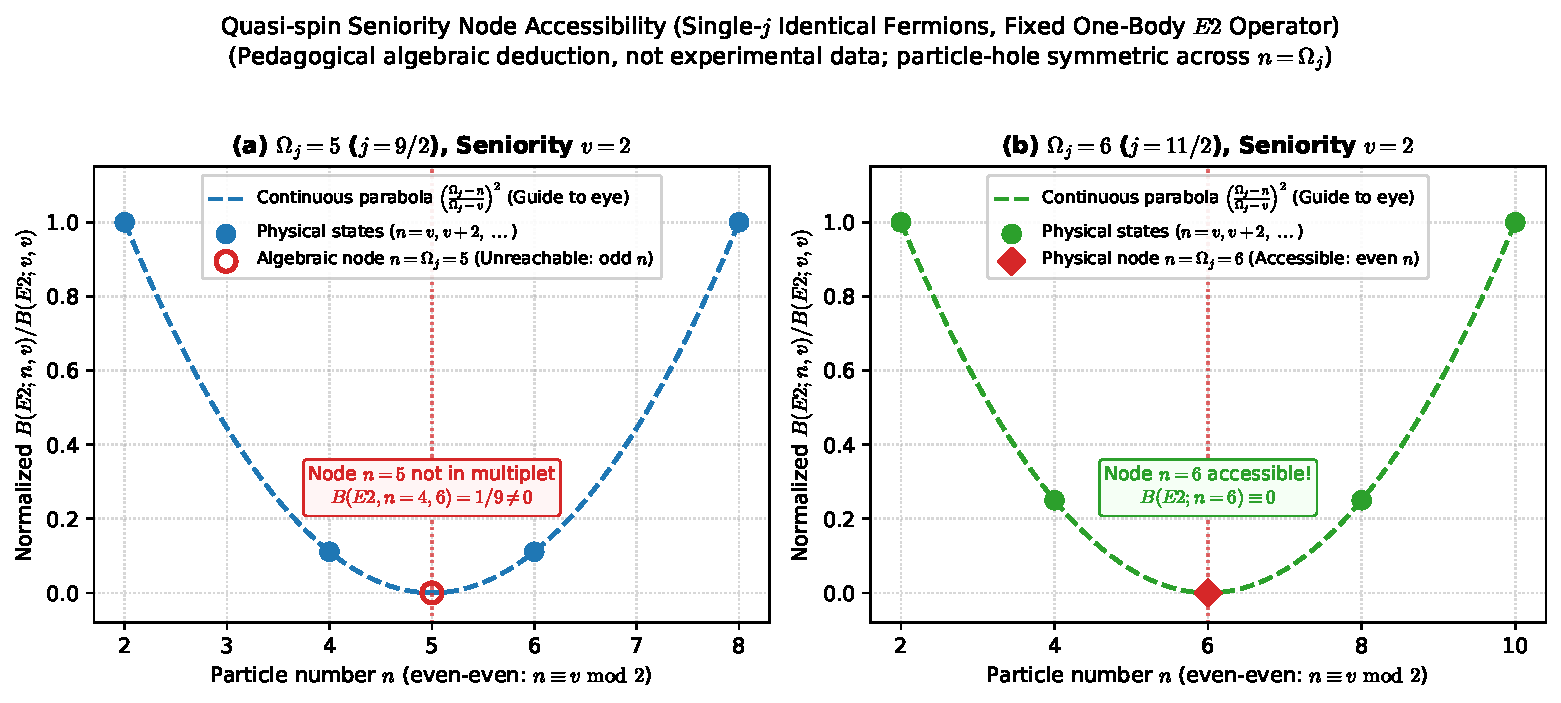
\includegraphics[width=0.88\textwidth]{Img/seniority-node-accessibility.pdf}
\caption[seniority节点的离散占据可达性]{单 $j$ 壳层同种费米子在固定 Seniority $v=2$ 下归一化电四极跃迁强度比 $B(E2; n, v) / B(E2; v, v) = [(\Omega_j - n)/(\Omega_j - v)]^2$ 的离散粒子数可达性对比（教学代数模型推论，非实验寿命预言）。(a) $\Omega_j = 5$（$j=9/2$），偶数 Seniority 家族（$n=2, 4, 6, 8$）永远无法取到奇数代数零点 $n=5$；(b) $\Omega_j = 6$（$j=11/2$），半满点 $n=6$ 为物理允许点，理论上精确击中相消节点。图线展现了跨半满壳 $n = \Omega_j$ 的粒子-空穴对称性。}\label{fig:seniority-node-accessibility}
\end{figure}
\item \textbf{准自旋单态边界（$v = \Omega_j$）：}
若考虑的状态具有最大未配对数 $v = \Omega_j$，则 $S = (\Omega_j - v)/2 = 0$，体系处于准自旋单态（Quasi-Spin Singlet）。此时式~\eqref{eq:4-6-seniority-reduction} 的分母 $\Omega_j - v = 0$ 出现未定义形式。这在物理上意味着准自旋标量态无法通过 $s=1$ 矢量算符实现相同 $S=0$ 态之间的非零耦合（Clebsch-Gordan 系数 $C_{0 0 1 0}^{0 0} \equiv 0$），其物理矩阵元直接由准自旋矢积选择定则决定，并不发生任何物理发散，也不意味着该核素仅存在唯一的量子态。
\item \textbf{算符适用范围规范：}
本推导严格建立在算符属于 $L>0$ 且为偶数的单体电张量算符（在粒子-空穴变换下反演而呈现准自旋矢量性）。该式\textbf{不能无条件推广至单粒子对角期待值或单体标量算符（如粒子数算符 $\hat{N}$ 或电单极算符 $E0$）}，因为标量算符包含非零的准自旋标量成分（$s=0$），其对角期望值具有完全不同的线性斜率。
\item \textbf{跨 Seniority 跃迁（$\Delta v = 2$）与真实多组态混合：}
根据准自旋空间 Wigner-Eckart 定理，张量秩 $s=1$ 的电算符除了连接 $S \to S$（$\Delta v = 0$）外，同样允许在 $|S - S'| = 1$（即改变未配对数 $\Delta v = \pm 2$）的状态之间产生非零矩阵元。对于 $\Delta v = 2$ 跃迁，其矩阵元随粒子数的演化规律与式~\eqref{eq:4-6-seniority-reduction} 截然不同，在半满壳 $n = \Omega_j$ 处并不相消。
在真实原子核中，多 $j$ 壳层组态混合、剩余两体有效电算符以及核芯四极极化微扰会改变相消的精确节点位置与曲线曲率。因此在实际能谱中，纯单 $j$ 壳层的理论零点通常演变为一个平缓或局域下沉的极小值，不能把所有同位素链上的极小化现象都机械当成严格纯单 $j$ 定理。
\end{enumerate}

\paragraph{典型案例剖析与粒子-空穴对称检验：}
考虑锡同位素链中的高自旋异能态。在纯中子 $1h_{11/2}$ 模型中，$\Omega_j=6$，半满节点是该轨道的粒子数 $n=6$。怎样把这一模型占据映射到具体同位素，还需其余价轨道的占据，不能由质量数直接指定。
而在接近中子闭壳的 $^{130}\mathrm{Sn}$（$N=80$）中，中子相当于在 $h_{11/2}$ 壳层容纳了 10 个中子（即 2 个中子空穴，对应 $n=10, v=2$）。将参数代入归约公式~\eqref{eq:4-6-seniority-reduction}：
\begin{equation}\label{eq:4-6-130sn-check}
\frac{\Omega_j - n}{\Omega_j - v} = \frac{6 - 10}{6 - 2} = \frac{-4}{4} = -1 \implies \left( \frac{\Omega_j - n}{\Omega_j - v} \right)^2 = (-1)^2 = 1.
\end{equation}
式~\eqref{eq:4-6-130sn-check} 给出了一个深刻的物理判据：\textbf{$^{130}\mathrm{Sn}$ 并非处于半满相消的零点上}！该式表明，$n=10$（两空穴）的单体 $B(E2)$ 在纯单 $j$ 极限下与 $n=2$（两粒子）的数值严格相同，体现的是粒子-空穴共轭对称性，而非半满相消抑制。
根据核数据评估记录（以 Singh 2001 年在 Nuclear Data Sheets 的采用能级数据快照为例~\cite{singh-2001-nds-130sn-adopted}），$^{130}\mathrm{Sn}$ 测得微秒级半衰期（$T_{1/2} = 1.61(15)\,\mu\mathrm{s}$）的高自旋态实际对应于激发能 $E_x = 2434.79(12)\text{ keV}$ 的 $(10^+)$ 态；该态通过一条低能 $E_\gamma = 96.54(5)\text{ keV}$ 的 $E2$ 射线退激至下方的 $(8^+)$ 态（$E_x = 2338.26(11)\text{ keV}$），采用的反演跃迁强度为 $B(E2) = 0.38(4)\,\text{W.u.}$，总内转换系数高达 $\alpha = 1.829$。需要明确，内转换过程本身的物理效应是增加总跃迁速率（$\lambda_{\mathrm{tot}} = (1+\alpha)\lambda_\gamma$），在给定 $B(E2)$ 与跃迁能量时实际上缩短了激发态的总寿命。该 $(10^+)$ 态之所以表现出微秒级长寿命，其核心物理原因在于跃迁能量极低（仅 $E_\gamma = 96.54\text{ keV}$），使得纯辐射相空间因子 $(E_\gamma)^5$ 受到极强压制，叠合了较小的约化跃迁强度（该 $B(E2) = 0.38(4)\,\text{W.u.}$ 属于核数据评价由寿命与理论转换系数反演导出的导出量，非独立的库仑激发测量）；其长寿命本质上是由低能相空间主导的自旋陷阱效应，绝不能机械看作半满壳相消的产物。而在真实锡同位素链中，从 $^{116}\mathrm{Sn}$ 到 $^{130}\mathrm{Sn}$ 跨越 14 个中子，单粒子能隙与形变相互作用使中子分布于多轨道中，不能简单将代数点 $n=6$ 与特定核素如 $^{122,124}\mathrm{Sn}$ 作刚性的一一对应，真实的极小值位置取决于多轨道占据与剩余相互作用。

\subsection{轴对称形变、K 选择定则与折合阻碍度}\label{sec:4-6-2}

当原子核脱离闭壳区进入稀土区或锕系区时，多核子关联驱动原子核自发产生宏观四极形变。在轴对称形变核的强耦合图景中，内禀参考系具有选定的空间对称轴（体轴 $3$ 轴）。各单核子的角动量投影量子数满足：
\begin{equation}\label{eq:4-6-omega-i-def}
\Omega_i = \Lambda_i + \Sigma_i,
\end{equation}
其中 $\Lambda_i$ 为单粒子轨道角动量投影，$\Sigma_i = \pm 1/2$ 为具有代数符号的内禀自旋投影。多准粒子内禀态在对称轴上的总角动量投影量子数满足代数和：
\begin{equation}\label{eq:4-6-K-def}
K = \sum_i \Omega_i.
\end{equation}
需强调，内禀投影 $K$ 严格不同于实验室系总角动量磁量子数 $M$。即便在静态轴对称形变（$\gamma = 0$）极限下，一旦原子核在转动坐标系中发生旋转，Coriolis 力与粒子-转子耦合依然会引入微扰破缺；因此 $K$ 在真实转动核中始终属于一种近似的好量子数。

当原子核发生多极度为 $\lambda$ 的电磁辐射跃迁时，发射光子在对称轴方向最多只能带走 $\lambda$ 个单位的角动量投影。根据第2.5节的角动量投影代数，从初态 $|I_i K_i\rangle$ 向末态 $|I_f K_f\rangle$ 的电磁跃迁遵守 \textbf{$K$ 选择定则}：
\begin{equation}\label{eq:4-6-K-selection-rule}
\Delta K \equiv |K_i - K_f| \le \lambda.
\end{equation}
当投影改变超过光子多极度时，单K极限中的相应矩阵元为零。这称为K禁戒；真实跃迁需通过混合等机制获得非零振幅。

定义电磁跃迁的 \textbf{$K$ 禁戒度（Degree of $K$-forbiddenness）} 为：
\begin{equation}\label{eq:4-6-forbiddenness-degree}
\nu \equiv \Delta K - \lambda.
\end{equation}
注意：$\nu$ 仅在 $\Delta K > \lambda$ 时定义（即 $\nu \ge 1$）；若 $\nu \le 0$，跃迁为 $K$ 允许跃迁，本概念不适用。

为了定量度量电磁跃迁受到的微观阻碍，实验上首先定义相对于同能量、同多极度的 Weisskopf 单粒子估计值的阻碍因子 $F_W$（Weisskopf Hindrance Factor）~\cite{book-jain-nuclear-isomers}：
\begin{equation}\label{eq:4-6-FW-def}
F_W \equiv \frac{\tau_\gamma(\mathrm{exp})}{\tau_\gamma(W)} = \frac{B_W(\sigma\lambda)}{B(\sigma\lambda; I_i \to I_f)},
\end{equation}
其中实验部分辐射寿命与第5.9节的测量定义严格对齐：若分支比采用包含内转换的总跃迁份额 $b_k^{\mathrm{tot}}$，则 $\tau_\gamma(\mathrm{exp}) = \tau_{\mathrm{exp}} (1 + \alpha_k) / b_k^{\mathrm{tot}}$；若分支比直接采用纯光子发射份额 $b_k^\gamma$，则 $\tau_\gamma(\mathrm{exp}) = \tau_{\mathrm{exp}} / b_k^\gamma$，不可重复乘入 $(1+\alpha)$ 因子。核物理学界引入每个禁戒度单元的平均阻碍率——\textbf{折合阻碍度（Reduced Hindrance per degree of $K$-forbiddenness）} $f_\nu$：
\begin{equation}\label{eq:4-6-fnu-def}
f_\nu \equiv (F_W)^{1/\nu} = \left[ \frac{\tau_\gamma(\mathrm{exp})}{\tau_\gamma(W)} \right]^{1/\nu}.
\end{equation}
式~\eqref{eq:4-6-fnu-def} 是对阻碍因子按禁戒度开根号的定义，适用于 $\nu>0$；它不是准自旋代数给出的普适微观幂律。与同能量、同多极度的Weisskopf估计比较，有助于区分相空间与矩阵元阻碍，但所得数值仍依赖具体支路。$K$ 混合也不限于三轴形状：轴对称平均场之外的Coriolis耦合及残余相互作用同样可能混合不同 $K$ 成分。

\paragraph{经典基准案例：$^{178}\mathrm{Hf}$ 的 $16^+$ 异能态：}
一个经典例子是 $^{178}\mathrm{Hf}$ 的 $K^\pi=16^+$ 异能态。Jain等人的部分能级图给出其能量为2446.1 keV、半衰期约31年；常用指派由质子和中子各一对准粒子构成：~\cite{book-jain-nuclear-isomers}
\begin{equation}\label{eq:4-6-178hf-config}
|\pi^2(7/2^+[404] \otimes 9/2^-[514]) \otimes \nu^2(7/2^-[514] \otimes 9/2^+[624])\rangle_{K=16}.
\end{equation}
同一图中，16$^+$态向 $K=8$ 带的连接涉及很小的能量差。例如到标为 $(13)^-$、2433.3 keV态的图示连接，端点差约12.8 keV；若以最低允许的E3分量讨论，名义禁戒度为 $16-8-3=5$。这项几何计算不能替代该支路多极性、部分光子分支和转换系数的实测或评价。图中的其它低能连接也提示：解释总半衰期必须同时处理低能相空间、内转换及构型阻碍。不能把级联中另一条495-keV光子直接当成16$^+$态的这一出口。

\subsection{三轴非轴对称形变与 K 混合动力学}\label{sec:4-6-3}

当原子核偏离轴对称形变（$\gamma \ne 0$）时，核形状呈现三轴椭球特征。体轴坐标系中的主轴不再具有轴向旋转守恒性，核子总角动量在体轴上的投影 $K$ 不再是严格守恒的好量子数。在正交粒子-转子模型（PRM）基底下，多体态必须展开为不同 $K$ 分量的相干叠加态：
\begin{equation}\label{eq:4-6-K-mixing-expansion}
|\Psi_M^I\rangle = \sum_{K} c_K |I M K\rangle, \quad \sum_K |c_K|^2 = 1.
\end{equation}
注意：若采用第2.5节与附录B中的非正交投影试探基底，展开系数必须通过度规重叠矩阵归一化，式~\eqref{eq:4-6-K-mixing-expansion} 的幺正归一形式严格对应于正交化后的有效粒子-转子基底。

考虑名义上具有高 $K_i$ 的异能态与名义上具有低 $K_f$ 的终态（满足 $\Delta K > \lambda$）。在波函数展开式~\eqref{eq:4-6-K-mixing-expansion} 下，跃迁矩阵元严格由双端混合分量的相干双重求和给出：
\begin{equation}\label{eq:4-6-K-mixed-matrix-element}
\langle \Psi_f^{I_f} || \hat{\mathcal{M}}(\lambda) || \Psi_i^{I_i} \rangle = \sum_{K, K'} c_{K'}^{(f)*} c_K^{(i)} \langle I_f K' || \hat{\mathcal{M}}(\lambda) || I_i K \rangle.
\end{equation}
根据电磁算符选择定则，单粒子矩阵元仅在 $|K - K'| \le \lambda$ 时非零。
\begin{enumerate}
\item \textbf{微弱杂化振幅维持有效阻碍：}
在单一主导退激路径的近似下，跃迁矩阵元取决于初态中掺入的微量低 $K$ 杂质分量（$c_{\mathrm{low}}^{(i)}$）或者终态中掺入的高 $K$ 杂质分量（$c_{\mathrm{high}}^{(f)}$）。由于三轴非轴对称势能曲面的束缚，这些非本征杂化振幅模方通常很小（$|c_K|^2 \ll 1$）。在主导分量占优时，跃迁速率近似标度为 $B(\sigma\lambda) \propto |c_{\mathrm{low}}^{(i)}|^2$ 或 $|c_{\mathrm{high}}^{(f)}|^2$。因此，三轴形变打开了 $K$ 混合通道，但只要非轴对称形变相对适中，杂化振幅的微小性仍然保证跃迁保留可观的阻碍度，绝不意味着三轴形变会使 $K$ 阻碍瞬间消失。
\item \textbf{反向推断非唯一性（反方检验）：}
反过来，若在实验中测得某异能态的折合阻碍度较小（如 $f_\nu < 10$），在科学逻辑上\textbf{严禁直接反推原子核必然存在静态三轴形变}。在真实核系统中，削弱 $K$ 阻碍存在多种平行的微观机制：
\begin{itemize}
\item \textbf{Coriolis 力带混合：} 转动参考系中 Coriolis 算符具有选择定则 $\Delta K = \pm 1$，随自旋升高逐级掺入低 $K$ 成分；
\item \textbf{高激发态密度统计混合：} 在高激发能区，核能级密度剧烈增加，复杂组态相互混合导致纯度下降；
\item \textbf{八极软度：} 空间反射对称破缺与八极振动亦可有效连接不同 $K$ 组态。
\end{itemize}
\end{enumerate}

在过渡核区 $A\approx 190$（Os、Ir、Pt 核素）中，三轴微观动力学展现出极佳的实验室样本。例如在过渡核区 $^{191}\mathrm{Ir}$ 的低能结构研究中，Lukasiak 等人采用粒子-三轴转子模型（PRM）分析了非轴对称势与转动能对低自旋能级及电磁跃迁几率的描述范围~\cite{continuation-g18-lukasiak-1979-191ir-triaxial-rotor}。然而必须指出，三轴粒子-转子模型对低激发集体态的成功描述，不能无条件外推为已从第一性微观上完整解释高自旋长寿命异能态（例如该核区激发能在 $2\text{ MeV}$ 以上的秒级长寿命异能态）；现有理论计算尚未在同组自洽波函数与同一组算符下闭环重现所有高禁戒退激分支比，高自旋异能态的微观组态纯度与三轴动力学响应依然具有明确的外推边界。

\subsection{形状异能态与双峰裂变位垒隧穿}\label{sec:4-6-4}

形状异能态涉及不同形状构型之间受抑制的转换。重核中的经典例子是裂变异能态；形状异能机制并不只限于这种情形。本小节先讨论具有第二形状势阱的裂变例子，其衰变需同时考虑构型重叠、势垒穿透及开放出口。

在超重核与锕系核中，斯楚廷斯基壳修正方法（Strutinsky Shell Correction）揭示：当原子核沿伸长轴拉伸时，液滴模型的光滑势能曲线与单粒子能隙的微观壳修正相叠加，在四极形变空间形成显著的双峰裂变位垒（Double-Humped Fission Barrier）~\cite{book-jain-nuclear-isomers}。其第一势阱对应正常形变基态（ND，$\beta_2 \approx 0.2\text{--}0.25$），内位垒 $V_A$ 隔离了大形变区域，第二势阱对应超形变极小态（SD，典型形变达到 $\beta_2 \approx 0.6$，长短轴比例接近经典的 $2:1$），外位垒 $V_B$ 则通向裂变鞍点。

处于第二极小态的形状异能态面临自发裂变（向外隧穿 $V_B$）与延迟 $\gamma$ 退激（向内隧穿 $V_A$ 回到第一势阱）的统计竞争。根据 WKB 半经典隧穿理论，穿透因子受到位垒作用量积分的指数级压制：
\begin{equation}\label{eq:4-6-WKB-tunneling}
\mathcal{P}_{\mathrm{tunnel}} \propto \exp\left( -\frac{2}{\hbar} \int_{s_{\mathrm{in}}}^{s_{\mathrm{out}}} \sqrt{2 \mathcal{M}(s) \left[ V(s) - E \right]} \, ds \right),
\end{equation}
其中 $\mathcal{M}(s)$ 为依赖于形状坐标的微观惯量参数，$V(s) - E$ 为位垒高度。要由穿透几率得到绝对衰变寿命，理论上还必须给定势阱内的尝试碰撞频率（Attempt Frequency）与前置因子。更重要的是，真实裂变异能态的寿命不仅取决于单维势垒的单纯穿透率，更取决于双峰势垒内复合门态（Doorway States）的共振杂化以及向内穿透辐射 $\gamma$ 退激与向外穿透自发裂变两个分支的竞争比。此外，超形变（$\beta_2 \approx 0.6$）与毫秒级半衰期仅是锕系裂变异能态的特征形态，不能将其作为所有核区全部形状异能态的先验定义。

\paragraph{典型基准发现与概念界限澄清：}
Jain等人的历史回顾叙述了Polikanov等在Dubna重离子实验中发现的延迟裂变：最初观测到约 $10^{-2}$ 秒的活动，后来与 $^{242}\mathrm{Am}$ 约2.2-MeV、14-ms的裂变异能态联系起来，并报告近乎全部经裂变退激。\cite{book-jain-nuclear-isomers} 这里引用的是综述对发现及后续评价的叙述，不能把所有数值倒写成早期一次测量的结果。在比较时还需区分：
\begin{itemize}
\item \textbf{状态身份}：同一核素还有约48-keV、半衰期约141年的低激发异能态；它与上述毫秒裂变态不是同一个态。不同出口及不同形状构型，能使同一核素呈现悬殊的寿命；
\item \textbf{形状共存与形状异能}：低能双 $0^+$ 态可以用于研究形状混合，但“两条 $0^+$ 能级”本身还不等于一个已建立的形状异能机制。需要寿命、E0/E2及模型约束；其中某些受阻转换可形成形状异能态，也不能自动套用锕系双峰裂变势垒。第4.2、4.3节的过渡核比较与这里的裂变例子应按各自观测量连接；
\item \textbf{隧穿阻碍与合成截面的独立性：} 异能态的长寿命仅反映形成之后在势阱内的生存几率，与重离子反应入射道熔合穿透及存活截面完全属于不同物理阶段。
\end{itemize}

\subsection{本节小结与两翼探针接口}\label{sec:4-6-5}

本节系统推演了同核异能态作为多体波函数选择探针的四重物理机制及其数学边界：
\begin{enumerate}
\item \textbf{四机制的电磁标度统一：} 异能态的长寿命根源于辐射跃迁速率式~\eqref{eq:4-6-rate-scaling} 中相空间因子 $(E_\gamma)^{2L+1}$ 的运动学压制（自旋陷阱）、几何代数矩阵元的结构抵消（Seniority 异能态）、空间对称轴角动量投影错位（$K$ 异能态）以及集体势能曲面位垒隧穿压制（形状异能态）。
\item \textbf{Seniority 半满相消：} 在同种核子单 $j$ 壳层中，$\Omega_j=(2j+1)/2$。单体偶多极电算符（$L>0$，如E2）在准自旋空间为秩1张量，$\Delta v=0$归约给出 $(\Omega_j-n)/(\Omega_j-v)$ 因子。其缩放公式要求 $v<\Omega_j$，半满零点还须属于该多重态的允许占据。$v=\Omega_j$须单独用准自旋选择定则处理，不能把公式的零分母解释为物理发散。多轨道混合与有效算符修正会改变实核的简单标度。
\item \textbf{K阻碍与混合：} $f_\nu=(F_W)^{1/\nu}$ 是 $\nu>0$ 时的定义。转移振幅应按初、末两端混合分量相干求和；只有某个小混合振幅主导时，才能近似得到相应模方标度。较小阻碍不能唯一反推三轴形变，Coriolis耦合和其它构型混合也需比较。
\item \textbf{形状异能态与位垒隧穿：} 锕系超形变第二极小态通过厚重位垒隧穿退激，具有 WKB 指数压制特征；必须严格将其与反应生成截面以及低能过渡核的双 $0^+$ 形状共存相区分。
\end{enumerate}

本节所确立的多体波函数选择定则，构筑了通向后续研究的清晰接口：
\begin{itemize}
\item \textbf{对第4.7节与第4.8节：} 弱衰变等待点与异能态热化是相关但不同的问题。例如 $^{130}\mathrm{Cd}$ 的beta衰变参与快过程流强，而 $^{180}\mathrm{Ta}^{\mathrm m}$ 的存活还取决于热网络的桥接与冷却历史。四类异能机制也可能在同一核态中叠加。
\item \textbf{对第5章：} 测量路线取决于寿命、反冲速度与探测响应。在相应敏感窗口内可使用DSAM、RDDS或快定时；更长延迟还可用束流时间结构、反冲输运及延迟符合测量。方法名称本身不规定所有核态都可达到的精度。
\end{itemize}
%
}{%
    \section{异能态对波函数的选择 [未完成]}\label{sec:4-6}%
    \textit{本节尚未完成。}%
}

%-- Section 4.7: 弱衰变与壳演化的互补探针
\setcounter{section}{6}%
\IfFileExists{Tex/Sections/sec-4-7.tex}{%
    \section{弱衰变与壳演化的互补探针}\label{sec:4-7}

在第2.2节中，我们阐明了单极相互作用与张量力驱动单粒子轨道漂移的壳演化微观机制；在第2.3节与第2.7节中，分别确立了 BCS 准粒子配对表象以及截断模型空间中有效电磁与弱跃迁算符的重整化规范；在第4.6节中，推演了同核异能态对多体波函数特定微观对称性与几何取向的选择定则。然而，电磁衰变与同核异能跃迁本质上属于同核内部不同激发态之间的电荷与电流响应，其质子数与中子数严格保持守恒。与此截然不同，弱相互作用 $\beta$ 衰变直接改变核内的质中比（$Z \to Z \pm 1$），能够在整条同量异位素链上横向探测单粒子波函数的占据几率、费米面附近的泡利阻塞效应以及集体运动自由度的微观重组。

这便引出了本节需要回答的核心问题：\textbf{弱相互作用衰变在何种机制下充当了原子核壳层演化、形状形变与超流配对的灵敏互补探针？实验观测到的有限衰变能窗、缓发粒子发射与双贝塔衰变矩阵元，如何对微观多体波函数施加严格的物理约束？}

本节划分为三个循序渐进的子模块：
\begin{enumerate}
\item \textbf{4.7.1节：Gamow-Teller、一阶禁戒与有限 Q 衰变能窗。} 将全 Hilbert 空间的几何代数和定则与实际有限能窗内的实测衰变速率严格区分，剖析原子核形变、轨道占据与粒子-振动耦合对跃迁强度的重分配与解阻塞效应，推演微分衰变能谱并界定守恒矢量流（CVC）的适用边界；
\item \textbf{4.7.2节：逐态 $\beta$ 缓发级联与中子多重度。} 阐述 $\beta$ 衰变前向馈送后高激发态在 $\gamma$ 辐射退激与中子发射之间的非相干统计级联竞争，给出发射几率的吸收级联概率分解，辨析不同文献中 $P_{1n}$、$P_{\ge 1n}$ 与平均多重度 $\langle M_n \rangle$ 的物理定义，纠正将 $Q_\beta - S_n$ 单纯当作充分预测公式的认识误区；
\item \textbf{4.7.3节：形变、配对与轻中微子 $0\nu\beta\beta$ 矩阵元范围。} 聚焦标准轻 Majorana 中微子交换机制，对比低能单 $\beta$ 衰变与双贝塔衰变在特征虚动量转移上的本质差异，阐述手征有效场论中 $\Delta L = 2$ 短程接触算符的重整化自洽性，剖析配对相干与四极形变错位对核矩阵元的调制作用。
\end{enumerate}

\subsection{Gamow-Teller、一阶禁戒与有限 Q 衰变能窗}\label{sec:4-7-1}

在第2.7节中，我们推导了完备状态空间中的裸单体 Gamow-Teller 算符与 Ikeda 差和定则：在 $t_3(n) = +1/2$、$t_3(p) = -1/2$ 与 $t_- |n\rangle = |p\rangle$（即 $\beta^-$ 跃迁降低核系统总同位旋第三分量 $T_3 = (N - Z)/2$）约定下，总跃迁强度定义为对所有可达末态的约化跃迁几率求和 $S_\mp \equiv \sum_{f_\mp} B(GT^\mp; J_i \to J_f) = \frac{1}{2J_i + 1} \sum_{f_\mp} |\langle f_\mp \| \sum_k \boldsymbol{\sigma}(k) t_\mp(k) \| J_i \rangle|^2$（约化跃迁几率 $B(GT^\pm)$ 的标准定义已包含初态自旋统计平均因子 $1/(2J_i + 1)$），由同位旋换位子 $[t_+, t_-] = 2 t_3$ 与全 Hilbert 空间完备闭合性给出 $S_- - S_+ = 3(N - Z)$。该定则是基于裸算符在无截断空间中导出的纯空间-同位旋几何代数恒等式，其裸定义本身完全独立于外在弱耦合常数 $g_A$ 及轻子运动学相空间加权。若引入常数有效淬灭因子 $q \equiv g_A^{\mathrm{eff}} / g_A^{\mathrm{bare}}$ 对单体 GT 矩阵元进行全局缩放，则差和相应按 $q^2$ 缩放为 $3 q^2 (N - Z)$；而在截断价空间（如准粒子 RPA 模型空间）中，差和定则的严格满足依赖于自旋-轨道劈裂伙伴轨道是否完全包含在模型空间内，且两体弱介子交换流（2BC）的引入将通过额外的微观代数项修正简单的单体求和。

在真实放射性衰变测量中，物理衰变速率严格受限于有限的衰变能释放窗（$Q$ 值）。采用中性基态原子质量 $M(A,Z)$，并暂略原子反冲与微小质量修正，有
\begin{align}
Q_{\beta^-}&=[M(A,Z)-M(A,Z+1)]c^2,\label{eq:4-7-Q-betaminus}\\
Q_{\beta^+}&=[M(A,Z)-M(A,Z-1)-2m_e]c^2,\label{eq:4-7-Q-betaplus}\\
Q_{\mathrm{EC}}&=[M(A,Z)-M(A,Z-1)]c^2.\label{eq:4-7-Q-EC}
\end{align}
前两式分别是 $\beta^-$、$\beta^+$ 的可用动能；$\beta^+$ 的开放条件为 $Q_{\beta^+}>0$。对捕获电子壳层 $j$、布居核激发能 $E_x$ 的分支，最终原子具有相应空穴，近似产生能量
\begin{equation}\label{eq:4-7-Q-EC-neutrino}
E_\nu(j,E_x)=Q_{\mathrm{EC}}-E_x-B_j
\end{equation}
的单色中微子；这里 $B_j$ 取子核对应的中性原子基态中该壳层电子的结合能。在运动学上，$\beta^-$ 衰变出射反中微子 $\bar{\nu}_e$，而 $\beta^+$ 衰变与电子俘获（EC）出射中微子 $\nu_e$；二者不可混写，亦不可将 $\beta^+$ 的 $-2m_e c^2$ 阈值套用到电子俘获之上。

根据弱相互作用有效拉氏量理论，出射带电轻子（动量为 $p_e$、总能量为 $E_e$）的微分发射速率公式写作：
\begin{equation}\label{eq:4-7-differential-spectrum}
\frac{d\lambda}{dW} = \frac{(G_F^{(E)})^2 |V_{ud}|^2 (m_e c^2)^5}{2\pi^3 \hbar} F(Z, W) p W (W_0 - W)^2 C(W),
\end{equation}
这里 $G_F^{(E)}$ 是自然单位制中以 $\mathrm{MeV}^{-2}$ 表示的费米常数，约为 $1.16638\times10^{-11}\,\mathrm{MeV}^{-2}$。式中 $m_e c^2$ 用能量单位，$\hbar$ 用能量乘时间单位，故前因子量纲为 $\mathrm{s}^{-1}$。若另用量纲为能量乘体积的 $G_F^{(\mathrm{SI})}$，才有 $G_F^{(E)}=G_F^{(\mathrm{SI})}/(\hbar c)^3$；不得对已用 $\mathrm{MeV}^{-2}$ 表示的常数再次除以 $(\hbar c)^3$。各运动学变量均以电子静止能量 $m_e c^2$ 无量纲化：
\begin{itemize}
\item $W \equiv 1 + \frac{T_e}{m_e c^2} = \frac{E_e}{m_e c^2}$ 为轻子无量纲总能量（$T_e$ 为轻子动能，$W \ge 1$）；
\item $p \equiv \frac{p_e c}{m_e c^2} = \sqrt{W^2 - 1}$ 为无量纲轻子动量；
\item $W_0 \equiv 1 + \frac{Q_\beta - E_x}{m_e c^2}$ 为对应于子核激发能为 $E_x$ 的特定退激分支的无量纲最大端点能量；
\item $F(Z, W)$ 为相对论 Fermi 函数，描述子核库仑势场对出射轻子波函数的连续态畸变（子核电荷取 $Z_{\mathrm{final}}$，对 $\beta^-$ 表现为库仑吸引 $F > 1$，对 $\beta^+$ 表现为库仑排斥且在低能端受阻遏）；
\item $C(W)$ 为谱形状因子（Shape Factor）。在无轨道角动量转移（$\Delta L = 0$）的允许跃迁中，若略去核子反冲修正、诱导流以及轻子波函数在核体积内的微小径向变化，形状因子可近似视为与能量无关的常数：
\begin{equation}\label{eq:4-7-shape-factor-allowed}
C_{\mathrm{allowed}}(W) \approx g_V^2 B(F) + g_A^2 B(GT),
\end{equation}
其中
\[
\begin{aligned}
 B(F)&=\frac{|\langle f\|\sum_k t_\pm(k)\|i\rangle|^2}{2J_i+1},\\
 B(GT)&=\frac{|\langle f\|\sum_k\boldsymbol\sigma(k)t_\pm(k)\|i\rangle|^2}{2J_i+1}.
\end{aligned}
\]
二者均采用单粒子同位旋算符 $t_\pm$（沿用第~2.7~节约定，且不含 $g_V$ 或 $g_A$），因而式~\eqref{eq:4-7-shape-factor-allowed} 中弱耦合常数只计一次。式~\eqref{eq:4-7-differential-spectrum} 为所述允许近似下的最低阶展开写法；弱电辐射修正（$\delta_R$）、核有限尺寸效应与非零核子反冲修正需按所采用的精度框架显式计入。在上述最低阶无量纲化约定下，式中的 Fermi 函数 $F(Z, W)$ 与形状因子 $C(W)$ 均为无量纲量；未加辐射修正的前因子常数 $K_0 \equiv \frac{2\pi^3 \hbar \ln 2}{(G_F^{(E)})^2 |V_{ud}|^2 (m_e c^2)^5} \approx 6292\,\mathrm{s}$（取 $G_F^{(E)} = 1.16638 \times 10^{-11}\,\mathrm{MeV}^{-2}$，$|V_{ud}| = 0.974$），与 Zhi 等采用的参考常数 $K = 6146\,\mathrm{s}$（如 Zhi 等~\cite{doctoral-r1-g34-zhi-2013-prc-shell-model-half-lives} 所用，其 Eq.(2) 给出了相应的相空间积分定义）有数值差异；比较时须核对弱耦合、辐射修正和强度定义，不能仅由此差值反推原文的修正组成。若引用已把 $(g_A/g_V)^2$ 吸收入 $B(GT)$ 的文献资料，亦应统一换算，不可重复乘入相同因子。此式针对指定 $\beta^\mp$ 分支；EC 应采用束缚电子波函数和离散中微子能量，不能直接套用连续 $\beta$ 谱。对能量积分得到的标准 Fermi 相空间因子 $f_0(Z, W_0) = \int_1^{W_0} F(Z, W) p W (W_0 - W)^2 dW$，其呈现的 $f_0 \propto Q_\beta^5$ 标度仅在超相对论与无库仑极限（$Z \to 0, W_0 \gg 1$）下成立，并非在全能量与全电荷区普遍精确的幂次。
\end{itemize}

在此需要澄清\textbf{守恒矢量流假设（CVC 假说）的微观适用范围}。CVC 假说断言弱矢量流与电磁同位旋流构成同一同位旋三态矢量，因此在同位旋对称性极限下，全空间积分配对的零动量总矢量荷算符 $\hat{T}_\pm = \int V_0^\pm d^3r$ 在核介质中不发生微观重整化。对于同位旋多重态之间的 Fermi 超允许跃迁，其矩阵元由同位旋升降算符代数严格给出：
\begin{equation}\label{eq:4-7-fermi-matrix-element}
\langle T, T_z \pm 1 | \hat{T}_\pm | T, T_z \rangle = \sqrt{T(T+1) - T_z(T_z \pm 1)}.
\end{equation}
文献中常见的 $\sqrt{2}$ 因子仅对应于 $T=1$ 同位旋三态（$T=1, T_z = \mp 1 \to T_z = 0$，如 $0^+ \to 0^+$ 超允许衰变）的特殊取值，不能直接推广到一般多重态。更重要的是，\textbf{CVC 假说对弱矢量流的保护严格体现在流守恒的场论微分恒等式中}：在零动量转移极限下，该守恒性确保了总时间分量弱矢量荷矩阵元不受强相互作用强重整化（$g_V = 1$）；而在有限动量转移下，CVC 假说进一步提供了空间矢量流与特定禁戒跃迁形状因子之间的微观代数联系（例如 Zhi 等~\cite{doctoral-r1-g34-zhi-2013-prc-shell-model-half-lives} 中依据 CVC 导出的矢量核矩阵元之间的一致性比例关系），但 CVC 并不能对弱轴矢量流提供相同的守恒保护。在有限动量转移、截断模型空间有效算符重整化以及库仑同位旋破缺效应下，弱矢量流矩阵元依然包含非平庸修正，不可将 CVC 误解为所有弱相互作用跃迁在核介质中均不受有效重整化。

在实际原子核能谱中，微观壳演化、形变与配对关联深刻调控着 Gamow-Teller 强度的能量分布：
\begin{enumerate}
\item \textbf{激发能级拓扑与有限能窗截断：} 在球形双闭壳核附近，很大一部分 Gamow-Teller 跃迁强度相干聚集在巨共振峰（GTGR）中。当 $Q_\beta$ 能窗显著低于巨共振能量时，衰变仅能布居其低能尾部，实测衰变速率直接受制于低能态的组态波包，不能单纯依据 $3(N-Z)$ 预测实际半衰期。
\item \textbf{四极形变与 Nilsson 轨道劈裂：} 原子核产生四极形变时，球形单粒子多重态劈裂为若干具有不同角动量投影 $\Omega$ 的 Nilsson 能级。这种单粒子谱的展宽使原本局域在高能区的 GT 强度发生碎裂并重构其能谱拓扑；形变引起的能级移动可对低能 $Q_\beta$ 衰变能窗内的强度产生重分配，其移动方向与强弱取决于费米面附近的具体单粒子轨道排布与组态结构，进而改变原子核的弱衰变半衰期。
\item \textbf{粒子-振动耦合（PVC）与多体强度的重分配：} 在纯单粒子壳模型或静态 RPA 计算中，若母核中子与子核质子的单粒子能级排布受到泡利不相容原理强烈阻遏，模型可能预言衰变能窗内的低能 GT 强度严格为零或极度微弱。然而正如 Wang 等在双闭壳核 $^{56}\mathrm{Ni}$、$^{100}\mathrm{Sn}$ 与 $^{132}\mathrm{Sn}$ 中的微观 RPA 与 PVC 联合计算所示~\cite{wang-2026-axial-coupling-quenching-joint-effects}，多粒子-多空穴关联与核芯表面振动声子相互作用对低能强度的重分布具有高度特异性：在自共轭核 $^{56}\mathrm{Ni}$ 中（涉及电子俘获衰变通道），引入 PVC 确实打破了闭壳冻结，在原本零强度的低能区产生微弱的解阻塞（Unblocking）强度；但在极丰中子双闭壳核 $^{132}\mathrm{Sn}$ 中，即便计入 PVC，采用 SGII Skyrme 相互作用在其实验物理 $Q_\beta$ 能窗内依然预言零 GT 强度（仅在 SkM* 参数下产生拖入能窗的微弱低能尾部），其实际半衰期仍主要受一阶禁戒跃迁主导。这表明微观多体关联不仅有淬灭效应，亦能引起强度的拓扑重分配，但不可将解阻塞效应过度推论为在所有双闭壳核中均普遍成立的开通机制。
\end{enumerate}

在远离稳定线的快中子俘获过程（$r$-过程）等待点核区，允许 Gamow-Teller 跃迁与一阶禁戒跃迁（First-Forbidden, FF，$\Delta \pi = -1$）的相对重要性随质量区发生显著演化。依据 Zhi 等人基于大尺度壳模型跨壳层计算的系统分析~\cite{doctoral-r1-g34-zhi-2013-prc-shell-model-half-lives}：
\begin{itemize}
\item 在 $N=50$（$Z \ge 28$，包括 $^{78}\mathrm{Ni}$）与 $N=82$（如 $^{130}\mathrm{Cd}$）等待点核区，Gamow-Teller 衰变仍然是主导衰变模式。例如在 $^{130}\mathrm{Cd}$ 中，计算证实 GT 衰变贡献了主导份额（采用有效淬灭因子 $q(GT) = 0.66$），一阶禁戒跃迁对计算半衰期的缩短贡献仅约 $13\%$；而在 $^{78}\mathrm{Ni}$ 中，独立粒子模型下中子 $1g_{9/2} \to \text{质子 } 1f_{7/2}$ 的 rank-1 FF 跃迁受到泡利阻塞，多体组态混合虽部分解除了这一阻塞，但在 $N=50$ 同中子素中 FF 贡献总体依然微弱（通常低于 $5\%$）。
\item 在 Zhi 等所研究的 $N=126$ 壳模型核素中，随质子数增加，GT 道因相关轨道的泡利阻塞而减弱；对于所算 $Z \ge 70$ 核素，FF 对半衰期的贡献超过 GT。这是该模型与核素范围内的结果，不是所有 $N=126$ 核素的普适结论。
\end{itemize}
以下只示意一阶禁戒算符的张量秩与宇称结构，动量写法取 $c=1$；实际数值计算需沿同一来源使用径向尺度和系数，不将不同量纲的示意算符直接相加。非相对论约化后包含的结构~\cite{doctoral-r1-g34-zhi-2013-prc-shell-model-half-lives}：
\begin{itemize}
\item 秩为 0 的类时轴荷算符：$\hat{\mathcal{O}}_0 \propto \gamma_5 \to \frac{\boldsymbol{\sigma} \cdot \mathbf{p}}{m_N}$，还包括 $[\mathbf r\otimes\boldsymbol\sigma]^{(0)}$ 型自旋偶极结构；
\item 秩为1的空间矢量与轴矢量结构：$\hat{\mathcal{O}}_1 \propto \mathbf{r}, \boldsymbol{\alpha} \to \frac{\mathbf{p}}{m_N}, \boldsymbol{\sigma}\times\mathbf{r}$；
\item 秩为 2 的空间张量算符：$\hat{\mathcal{O}}_2 \propto [\boldsymbol{\sigma} \times \mathbf{r}]_2$。
\end{itemize}
Zhi 等人在微观壳模型中表明：软 $\pi$ 介子交换流使类时轴荷算符表现出介质增强（拟合有效参数 $q(\xi' v) = 1.266 > 1$），而空间分量算符则呈现出不同程度的淬灭（秩 1 矢量算符 $q(x) = 0.51$，秩 1 轴矢量算符 $q(u) = 0.38$，秩 0 轴矢量算符 $q(w) = 0.66$，秩 2 张量算符 $q(z) = 0.42$）~\cite{doctoral-r1-g34-zhi-2013-prc-shell-model-half-lives}。对未极化初态、末态磁量子数未观测且轻子角度已积分的微分能谱，式~\eqref{eq:4-7-differential-spectrum} 中的形状因子 $C(W)$ 依赖电子能量，各核张量秩的贡献分块相加；同秩内不同算符矩阵元可相干干涉，例如秩 1 的 $x$ 与 $u$。这一结论限于上述能谱，不排除极化或角关联观测量中的其他干涉；单一标量淬灭因子仍不能简单推广至所有禁戒通道。

\subsection{逐态 $\beta$ 缓发级联与中子多重度}\label{sec:4-7-2}

当原子核极度偏离稳定线走向极丰中子区时，核质量差 $Q_\beta$ 显著升高，而子核的中子分离能 $S_n$（以及多中子分离阈值 $S_{2n}, S_{3n}$）则因过剩中子结合减弱而降低。当满足动学条件 $Q_\beta > S_n$ 时，母核通过 $\beta$ 衰变能够布居到子核中子分离阈值之上的激发态。这些处于非束缚连续谱中的激发能级随后迅速退激，产生 \textbf{$\beta$ 缓发中子发射（$\beta$-delayed neutron emission）}~\cite{dimitriou-2021-iaea-beta-delayed-neutron-database}。

在弱布居与后续退激可分离、各步能用非负部分宽度描述且相干干涉可忽略的近似下，$\beta$ 缓发粒子发射可以表示为两阶段的条件概率模型：
\begin{enumerate}
\item \textbf{弱馈送：} 令 $I_\beta(i)$ 为每次母核总衰变中直接馈送子核激发态 $i$ 的无量纲概率，离散态求和并包含连续谱积分后满足母核衰变分支比归一：
\begin{equation}\label{eq:4-7-beta-feeding-normalization}
\sum_i I_\beta(i) = b_\beta \le 1.
\end{equation}
若母核还存在自发裂变、$\alpha$ 衰变或结团发射等竞争道，则 $\beta$ 衰变分支比 $b_\beta < 1$。
\item \textbf{级联退激与吸收马尔可夫链：} 子核处于激发能高于中子分离阈的状态时，通过中子发射与辐射 $\gamma$ 级联竞争退激。令 $\Pi_x(a)$ 为处于激发态 $a$ 的体系经过相继退激级联最终总共释放 $x$ 个中子的净吸收概率。对于任意非终止的瞬态能级 $a$，$\Pi_x(a)$ 满足离散差分递推关系：
\begin{equation}\label{eq:4-7-cascade-pi-def}
\Pi_x(a) = \sum_{b, r} \frac{\Gamma^{(r)}_{a \to b}}{\Gamma_{\mathrm{tot}}(a)} \Pi_{x-r}(b), \qquad \Pi_{x < 0}(a) \equiv 0,
\end{equation}
其中 $\Gamma^{(r)}_{a \to b}$ 为从状态 $a$ 释放 $r$ 个中子（$r = 0, 1, 2, \dots$）跃迁至状态 $b$ 的部分衰变宽度，$\Gamma_{\mathrm{tot}}(a)$ 为该态全部开放通道的总退激宽度。对于被选定为终止退激的吸收态 $t$（如在所选观测时窗内不再释放中子的子核束缚基态或长寿命同核异能态），满足边界条件 $\Pi_x(t) = \delta_{x0}$。当所列通道在选定时窗内几乎必然完全吸收时，全多重度概率守恒 $\sum_{x \ge 0} \Pi_x(a) = 1$。

按每次母核总衰变归一的 $\beta$ 缓发 $x$ 中子发射净分支比，以及按 $\beta$ 衰变事件条件归一的中子发射几率分别定义为：
\begin{equation}\label{eq:4-7-conditional-probability}
P_{xn}^{(\beta;\mathrm{parent})} = \sum_i I_\beta(i) \Pi_x(i), \qquad P_{xn}^{(\beta \mid \beta)} = \frac{P_{xn}^{(\beta;\mathrm{parent})}}{b_\beta} \quad (b_\beta > 0).
\end{equation}
前者对所有发射中子数求和等于母核 $\beta$ 衰变分支比 $\sum_{x \ge 0} P_{xn}^{(\beta;\mathrm{parent})} = b_\beta \le 1$，后者则满足条件全概归一 $\sum_{x \ge 0} P_{xn}^{(\beta \mid \beta)} = 1$。
\end{enumerate}
仅在略去多步相继发射（$r \le 1$）且假定阈上 $\gamma$ 衰变全部直达束缚态（$\Pi_1(\text{束缚}) = 0$）的极简单步极限下，能级 $i$ 的发射吸收概率才退化为单步分支比 $\Pi_1(i) \approx \frac{\Gamma_n(i)}{\Gamma_{\mathrm{tot}}(i)}$。

\begin{figure}[!htbp]
\centering
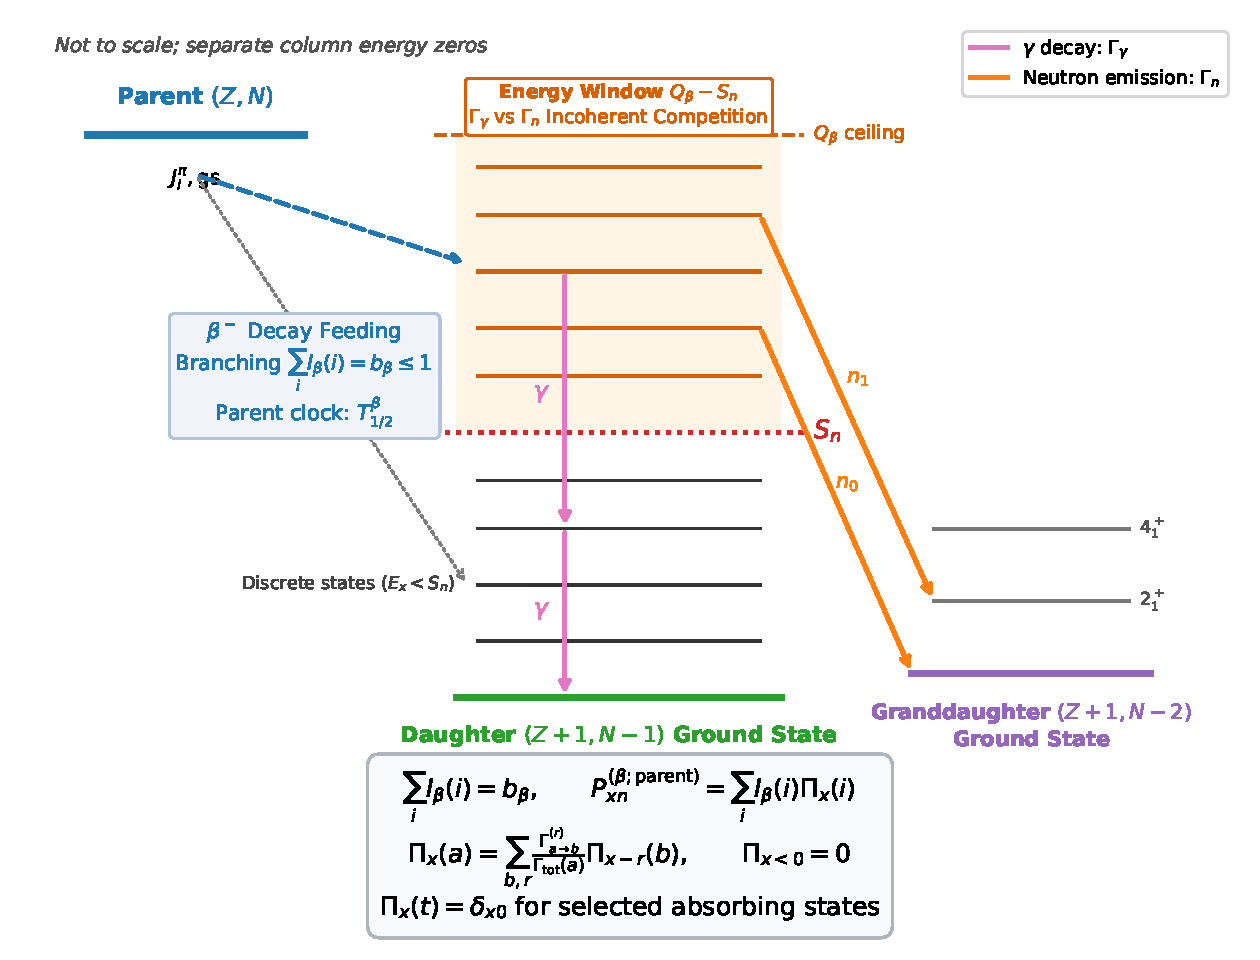
\includegraphics[width=0.98\textwidth]{Img/weak-cascade-competition.pdf}
\caption[前驱母核 $(Z, N)$ 经 $\beta^-$ 衰变馈送至子核 $(Z+1, N-1)$ 高激发态后，在能量窗口 $Q_\beta - S_n$ 内中子发射通道与辐射退激通道的非相干统计级联竞争示意图]{前驱母核 $(Z, N)$ 经 $\beta^-$ 衰变馈送至子核 $(Z+1, N-1)$ 高激发态后，在能量窗口 $Q_\beta - S_n$ 内中子发射通道与辐射退激通道的非相干统计级联竞争示意图（教学原理模型，展示衰变母态分支比归一与级联退激吸收网络，非特定实验装置原始计数）。}\label{fig:weak-cascade-competition}
\end{figure}

式~\eqref{eq:4-7-conditional-probability} 与图~\ref{fig:weak-cascade-competition} 澄清了理论分析中的一个\textbf{关键认识误区}：
\begin{quote}
\textbf{$Q_{\beta n}\equiv Q_\beta-S_n$ 给出单中子通道的可用能量窗口；它本身并不能充分预测中子发射几率 $P_n$。}
\end{quote}
即便子核能级位于中子分离阈值之上（$E_x(i) > S_n$），发射中子也并不具有绝对的必然性。如果激发能仅仅略微高出 $S_n$（出射中子能量极低），而由于初态能级与孙核低激发态之间的自旋宇称匹配要求中子必须携带较高的轨道角动量（如 $l=2$ 或 $l=3$），出射中子波函数将遭受离心势垒（Centrifugal Barrier $V_l = \frac{\hbar^2 l(l+1)}{2\mu r^2}$）的显著阻碍，导致中子发射受到明显抑制。此时，辐射 $\gamma$ 衰变仍然能够有效竞争，使核退激回到子核的束缚基态。此外，当跨越壳层闭合点时，单粒子能隙突变会导致 $Q_\beta$ 与 $S_n$ 发生阶跃式变化，使实际测量的中子发射概率呈现出非连续突变。

在核数据评估与实验测量中，必须严格区分国际原子能机构（IAEA）参考数据库所规范的不同物理定义~\cite{dimitriou-2021-iaea-beta-delayed-neutron-database}：
\begin{enumerate}
\item \textbf{单中子发射几率 $P_{1n}$：} 每次前驱母核总衰变中，恰好释放 1 个中子的净分支几率：
\begin{equation}\label{eq:4-7-P1n-def}
P_{1n}^{(\beta;\mathrm{parent})} = \sum_{i} I_\beta(i) \Pi_1(i);
\end{equation}
\item \textbf{全缓发中子发射总几率 $P_{\ge 1n}$（文献中常通称 $P_n$）：} 每次母核衰变发射至少 1 个中子的总几率：
\begin{equation}\label{eq:4-7-P-atleast-1n-def}
P_{\ge 1n}^{(\beta;\mathrm{parent})} = \sum_{x \ge 1} P_{xn}^{(\beta;\mathrm{parent})} = P_{1n}^{(\beta;\mathrm{parent})} + P_{2n}^{(\beta;\mathrm{parent})} + \dots;
\end{equation}
\item \textbf{平均缓发中子多重度 $\langle M_n \rangle$：} 每次母核衰变平均释放的中子数目：
\begin{equation}\label{eq:4-7-mean-multiplicity-def}
\langle M_n \rangle^{(\beta;\mathrm{parent})} = \sum_{x \ge 1} x P_{xn}^{(\beta;\mathrm{parent})} = P_{1n}^{(\beta;\mathrm{parent})} + 2 P_{2n}^{(\beta;\mathrm{parent})} + 3 P_{3n}^{(\beta;\mathrm{parent})} + \dots.
\end{equation}
\end{enumerate}
当多中子发射道闭合时（$Q_\beta < S_{2n}$），$P_{1n}^{(\beta;\mathrm{parent})} = P_{\ge 1n}^{(\beta;\mathrm{parent})} = \langle M_n \rangle^{(\beta;\mathrm{parent})}$；但在极丰中子核区，$P_{2n}$ 与 $P_{3n}$ 通道开启，三者的数值产生系统性偏离，数据分析时必须根据具体实验观测量进行精确映射。若研究按 $\beta$ 事件条件归一的中子几率，只需将上述各式除以母核分支比 $b_\beta$。

在这里采用的快退激近似下，缓发中子的主要延迟跟随前驱母核的弱衰变时钟；随后子核的中子发射与辐射竞争通过前述级联宽度处理。若某条通道存在不可忽略的额外延迟，应将其纳入时间演化，不能仍把全部时间分布归给母核。中子的飞行、热化和探测器俘获响应则属于另外的测量时间卷积。

设 $R_{y|x}$ 为真实发射 $x$ 个中子后探测系统记录到 $y$ 个信号的条件概率响应矩阵，则无门控母衰变观测到的中子多重度分布满足 $p_y^{\mathrm{obs}} = \sum_x R_{y|x} P_{xn}^{(\beta;\mathrm{parent})} + p_y^{\mathrm{non\text{-}}\beta}$。若母核同时存在自发裂变或带电粒子发射等竞争道，必须将其独立的中子多重度分布与探测器响应单独计入 $p_y^{\mathrm{non\text{-}}\beta}$ 项中，不可将非 $\beta$ 产中子道混同为 $\beta$ 缓发中子，亦不可将所有非 $\beta$ 衰变默认归入 $x=0$ 无中子模式。在理想单粒子效率 $\epsilon_n$、无串扰且忽略多重偶然计数的二项响应近似下，$R_{y|x} = \binom{x}{y} \epsilon_n^y (1 - \epsilon_n)^{x-y}$。实际测量中探测效率显著依赖于出射中子连续能谱、角分布与探测时间关联门，必须通过精准的源标定与 Monte Carlo 输运模拟构建响应矩阵，并通过贝叶斯前向似然或统计非折叠（Unfolding）算法提取真实发射多重度。

\subsection{形变、配对与轻中微子 $0\nu\beta\beta$ 矩阵元范围}\label{sec:4-7-3}

若确认 $0\nu\beta\beta$，在通常局域量子场论框架下将表明轻子数不守恒（$\Delta L = 2$），并通过 Schechter-Valle 黑盒论证确立中微子具有非零 Majorana 质量项；单凭衰变寿命观测本身不能独立证明轻中微子质量机制必定压倒重轻子或超对称等竞争机制，亦不能脱离微观核矩阵元唯象反演有效 Majorana 质量。在标准轻 Majorana 中微子交换占主导的理论假设下，物理过程由核内两个弱流顶点之间交换一条虚中微子传播子所驱动，理论半衰期可写作如下相容的因式分解形式：
\begin{equation}\label{eq:4-7-0nubb-halflife}
[T_{1/2}^{0\nu}]^{-1} = G_{0\nu} g_A^4 |M_{0\nu}|^2 \left|\frac{m_{\beta\beta}}{m_e}\right|^2, \qquad m_{\beta\beta} \equiv \left| \sum_j U_{ej}^2 m_j \right|.
\end{equation}
式中相空间因子 $G_{0\nu}$（以 $\mathrm{yr}^{-1}$ 为单位）按本式定义为已外提无量纲轴矢量常数因子 $g_A^4$；有效质量 $m_{\beta\beta}$ 与电子质量 $m_e$ 采用相同的质量或静止能量单位（使质量比无量纲）；微观核矩阵元 $M_{0\nu}$ 的多极展开、核子电弱形状因子、有限核半径 $R = 1.2 A^{1/3}\,\mathrm{fm}$ 标度规范必须与相空间因子 $G_{0\nu}$ 保持严格相容~\cite{engel-menendez-2017-double-beta-matrix-elements-review}。若文献定义吸收了耦合因子的相空间 $\widetilde{G}_{0\nu} \equiv G_{0\nu} g_A^4$，则外部不可重复乘入 $g_A^4$。
传统长程部分可写成
\begin{equation}\label{eq:4-7-NME-decomposition}
M_{0\nu}^{\mathrm{long}}=M_{GT}-\left(\frac{g_V}{g_A}\right)^2M_F+M_T.
\end{equation}
该轻中微子单线虚交换在核内涉及宽广的虚拟动量积分谱，其动量转移峰值位于 $|\mathbf{q}| \sim 100\text{--}200\,\mathrm{MeV}/c$（对应核子间距 $r \sim 1\text{--}2\,\mathrm{fm}$），在特征尺度上远远超出了单 $\beta$ 衰变的长波长零动量极限。
Cirigliano 等在基于手征有效场论对两核子 $^1S_0$ 散射非微扰重整化的分析中指出~\cite{cirigliano-2018-leading-short-range-double-beta}：单独的长程单中微子交换势 $V_\nu^{\mathrm{long}} \sim 1/r_{12}$ 会引入依赖于截断尺度的紫外发散；为了在两核子非微扰散射中满足重整化群自洽性，手征领头阶（LO）需引入一个 $\Delta L = 2$ 的两核子短程接触相互作用势。Cirigliano 等在文献中以 $\tau_{1,+} \tau_{2,+}$ 标示 $n n \to p p$ 同位旋跃迁；转换至本节所用的同位旋约定（$t_3(n) = +1/2, t_- |n\rangle = |p\rangle$），在剥离弱耦合与轻子因子后，其在自然单位制与坐标空间中的 $^1S_0$ 剥离相互作用势写作 $V_{\mathrm{CT}}^{(R)}(\mathbf{r}_{12}) = -2 g_\nu^{NN}(R) \delta_R^{(3)}(\mathbf{r}_{12}) t_{1,-} t_{2,-}$。该接触项的有效强度 $g_\nu^{NN}$ 具有正规化方案依赖性；现有文献尝试利用电荷独立性破缺（CIB）电磁数据约束反项低能常数组合（$C_1 + C_2$），但要确定单一耦合 $g_\nu^{NN} = C_1$ 仍需引入额外对称性假设（如 $C_1 \approx C_2$）或与格点 QCD 匹配，不能单凭该电磁数据直接唯一标定。该接触项属于 $\Delta L = 2$ 的双核子超弱通道，与单 $\beta$ 衰变中源自介子交换流的两体轴流（2BC）具有不同的物理机制。

原子核的微观波函数——特别是配对与形变——对 $M_{0\nu}$ 起着关键的调制与选择作用：
\begin{itemize}
\item \textbf{超流配对关联的相干性：} 双贝塔衰变将两个初态配对核子转换为两个末态配对核子。超流 BCS 凝聚态中同位旋矢量（$T=1$）核子对的相干叠加能够有效增大矩阵元；然而，若体系中存在较强的同位旋标量（$T=0$）质中配对竞争，不同配对道之间的干涉反而可能对矩阵元产生削弱效应。
\item \textbf{四极形变错位的微观压制：} 多数候选双贝塔衰变核处于球形到形变的过渡区。若母核与子核在自洽能量曲面上表现出不同的形变极小（例如长椭球母核衰变到扁椭球或弱形变子核），初末态微观内禀波函数在形状坐标空间中将出现波包错位。这种内禀波函数重叠的减弱，会对核矩阵元产生显著的压制效应，其具体压制幅度高度依赖于所选用的微观形变模型。
\item \textbf{反演非唯一性与微观不确定度：} 实验上测量到的双贝塔半衰期下限，是相空间、有效 Majorana 质量、有效轴矢量耦合 $g_A$ 以及多体波函数重叠共同作用的标量结果。从单一的半衰期测量值无法唯一反演局域形变参数或确定的 $g_A$ 淬灭数值，需结合电荷交换反应、双 Gamow-Teller 激发实验以及双核子转移反应等独立手段，对初末态的组态波函数施加协同约束。
\end{itemize}

\subsection{本节小结与微观探针接口}\label{sec:4-7-4}

本节确立了弱相互作用作为低能原子核结构、壳演化与微观关联多维探针的理论图像：
\begin{enumerate}
\item \textbf{有限能窗与强度分布重塑：} 实测 $\beta$ 衰变速率受限于有限能窗 $Q_\beta$ 与微分相空间谱。CVC 假说在零动量转移极限下保证弱矢量荷不受强相互作用强重整化，并在有限动量下约束矢量流，但不保护轴矢量流；四极形变引起 Nilsson 轨道劈裂重构 GT 巨共振分布，而粒子-振动耦合（PVC）在特定闭壳核组态下能够重构低能强度（但在不同核素与相互作用下表现各异，例如 $^{132}\mathrm{Sn}$ 在 SGII 下能窗内仍无 GT 强度）。在 $N=50, 82$ 区 GT 跃迁依然主导；而在 Zhi 等壳模型研究的 $N=126$ 核素中（$Z \ge 70$），随质子数增加 GT 因泡利阻塞减弱，FF 贡献反超 GT（受限于具体模型与核素范围）。
\item \textbf{缓发级联的两阶段统计竞争：} $\beta$ 缓发中子发射遵循条件概率分解式 $P_{xn}^{(\beta;\mathrm{parent})} = \sum_i I_\beta(i) \Pi_x(i)$ 及式~\eqref{eq:4-7-cascade-pi-def} 的逐步计数递推。能量差 $Q_\beta - S_n$ 仅设定理论上限，高于 $S_n$ 的能级仍面临离心势垒阻碍下的辐射 $\gamma$ 竞争退激；必须在定义与测量上严格区分按母核总衰变归一的 $P_{xn}^{(\beta;\mathrm{parent})}$ 与按 $\beta$ 衰变条件归一的 $P_{xn}^{(\beta\mid\beta)}$，以及单中子发射率 $P_{1n}$、全发射率 $P_{\ge 1n}$ 与平均中子多重度 $\langle M_n \rangle$。
\item \textbf{高动量转移下 $0\nu\beta\beta$ 矩阵元特征：} 在本文所述的标准轻 Majorana 中微子交换机制下，衰变由核内两核子弱流顶点之间交换一条虚中微子传播子所驱动，其特征虚动量转移达到 $|\mathbf{q}| \sim 100\text{--}200\text{ MeV}/c$（对应短程 $1\text{--}2\text{ fm}$）；手征有效场论非微扰散射的重整化要求引入领头阶 $\Delta L = 2$ 短程接触算符，其低能常数可借核子--核子散射中的电荷独立性破缺数据约束但不可由该数据单独唯一确定；配对相干与形变错位对核矩阵元产生竞争性调制，不可由单一寿命结果反向推断唯一的形变或淬灭参数。
\end{enumerate}

本节建立的弱衰变理论模型，构筑了以下跨章理论接口：
\begin{itemize}
\item \textbf{对第4.8节（核天体物理反应网络与开放系统演化）：} 极丰中子核素的实际 $\beta$ 衰变半衰期与缓发中子多重度 $\langle M_n \rangle$，与中子俘获/光致蜕变反应率、核质量以及天体环境的温度、中子密度和膨胀时间尺度等动力学参数共同影响着快中子俘获过程（$r$-过程）的反应路径走向与元素丰度峰位置分布；
\item \textbf{对第5章（在束实验谱学技术链）：} 母核的弱衰变时钟与出射中子的飞行、热化及俘获响应属于不同的时间演化环节；在束与放射性束流实验中，全吸收谱仪（TAGS）与中子探测阵列需结合母核衰变周期、能谱特性及时间关联门进行本底抑制与符合测量，并通过构建探测响应矩阵反演真实馈送与多重度分布。
\end{itemize}
%
}{%
    \section{弱衰变与壳演化的互补探针 [未完成]}\label{sec:4-7}%
    \textit{本节尚未完成。}%
}

%-- Section 4.8: 环境和形成路径怎样改变可见性
\setcounter{section}{7}%
\IfFileExists{Tex/Sections/sec-4-8.tex}{%
    \section{环境和形成路径怎样改变可见性}\label{sec:4-8}

在前述各节的讨论中，原子核的多体波函数、集体形变与跃迁算符通常是在零温自由空间（真空中的裸核多体系统）的微观模型边界下定义的；而实验谱学测量的衰变寿命与分支比，则是在特定的原子与外在介质环境（例如实验室常温下的中性原子、靶基底或晶格介质）中获得的。在第4.6节中，我们讨论了同核异能态的微观阻碍机制——自旋陷阱、Seniority 相消、高 $K$ 空间取向禁戒以及超形变第二极小波函数在变形空间中的位垒穿透压制~\cite{book-jain-nuclear-isomers}；在第4.7节中，探讨了弱衰变算符在有限相空间中的求和定则与有效衰变常数。当把微观核模型导出的核态性质应用于复杂实验与天体物理环境时，需要澄清一种直觉误区：即认为一个同核异能态在实验室中性原子或冷靶环境中拥有长达数小时乃至数年的半衰期，或者拥有更高的微观裂变位垒，便必然能够在高温恒星等离子体中长久存活，或在重离子熔合反应中必然对应更大的产生截面。

原子核在真实物理环境中的有效寿命与在实验谱学中的物理可见性，不是由孤立核哈密顿量单独决定的内禀常数，而是由原子核内禀结构、周围热力学与电磁场环境（辐射场光子密度、原子电离度、电子轨道占有数、晶格介电环境）以及动力学反应形成路径共同塑造的开放动力学过程。同一个核态，在冷真空环境中可能是长寿命异能态，但在高温恒星内部的光子浴中，却可以通过高能中间桥态的热共振激发起发生跨带混合，使有效寿命显著缩短；在原子内转换通道被强电离剥离或受晶格介电禁带压制的环境中，其寿命又可能因电子通道的关闭而延长；而在重离子熔合反应中，高自旋异能组态即使在低温势能面上具有较高的裂变位垒，也并不等同于高温高激发能下复合核的存活几率或最终蒸发剩余核截面会相应增大。

为了建立清晰且定量的物理图像，本节将环境与反应形成对原子核可见性的重塑解构为三个物理子模块：第\ref{sec:4-8-1}小节推演天体等离子体热辐射浴中的开放速率网络、成对可逆电磁跃迁的微观详细平衡边界以及跨簇热化时间尺度；第\ref{sec:4-8-2}小节解构原子核与核外电子通道的微观竞争，系统梳理自发辐射、内转换（IC）、电子俘获核激发（NEEC）、非弹性电子散射（NEIES）与电子跃迁核激发（NEET）等过程，并以 $^{229}\mathrm{Th}$ 光学核钟与 $^{93m}\mathrm{Mo}$ 诱发退激争议为原件实例，确立理论计算与实验证据的边界；第\ref{sec:4-8-3}小节推导重离子完全熔合蒸发反应的三阶段截面分波框架，明确入射势垒穿透、复合核形成与逐级蒸发存活的物理机制与不确定度，并辨析异能态冷态微观位垒与高温反应生成截面之间的逻辑脱耦。图~\ref{fig:4-8-environment-network}给出了这三个子模块的物理机制与特征通道示意图。

\begin{figure}[!htbp]
\centering
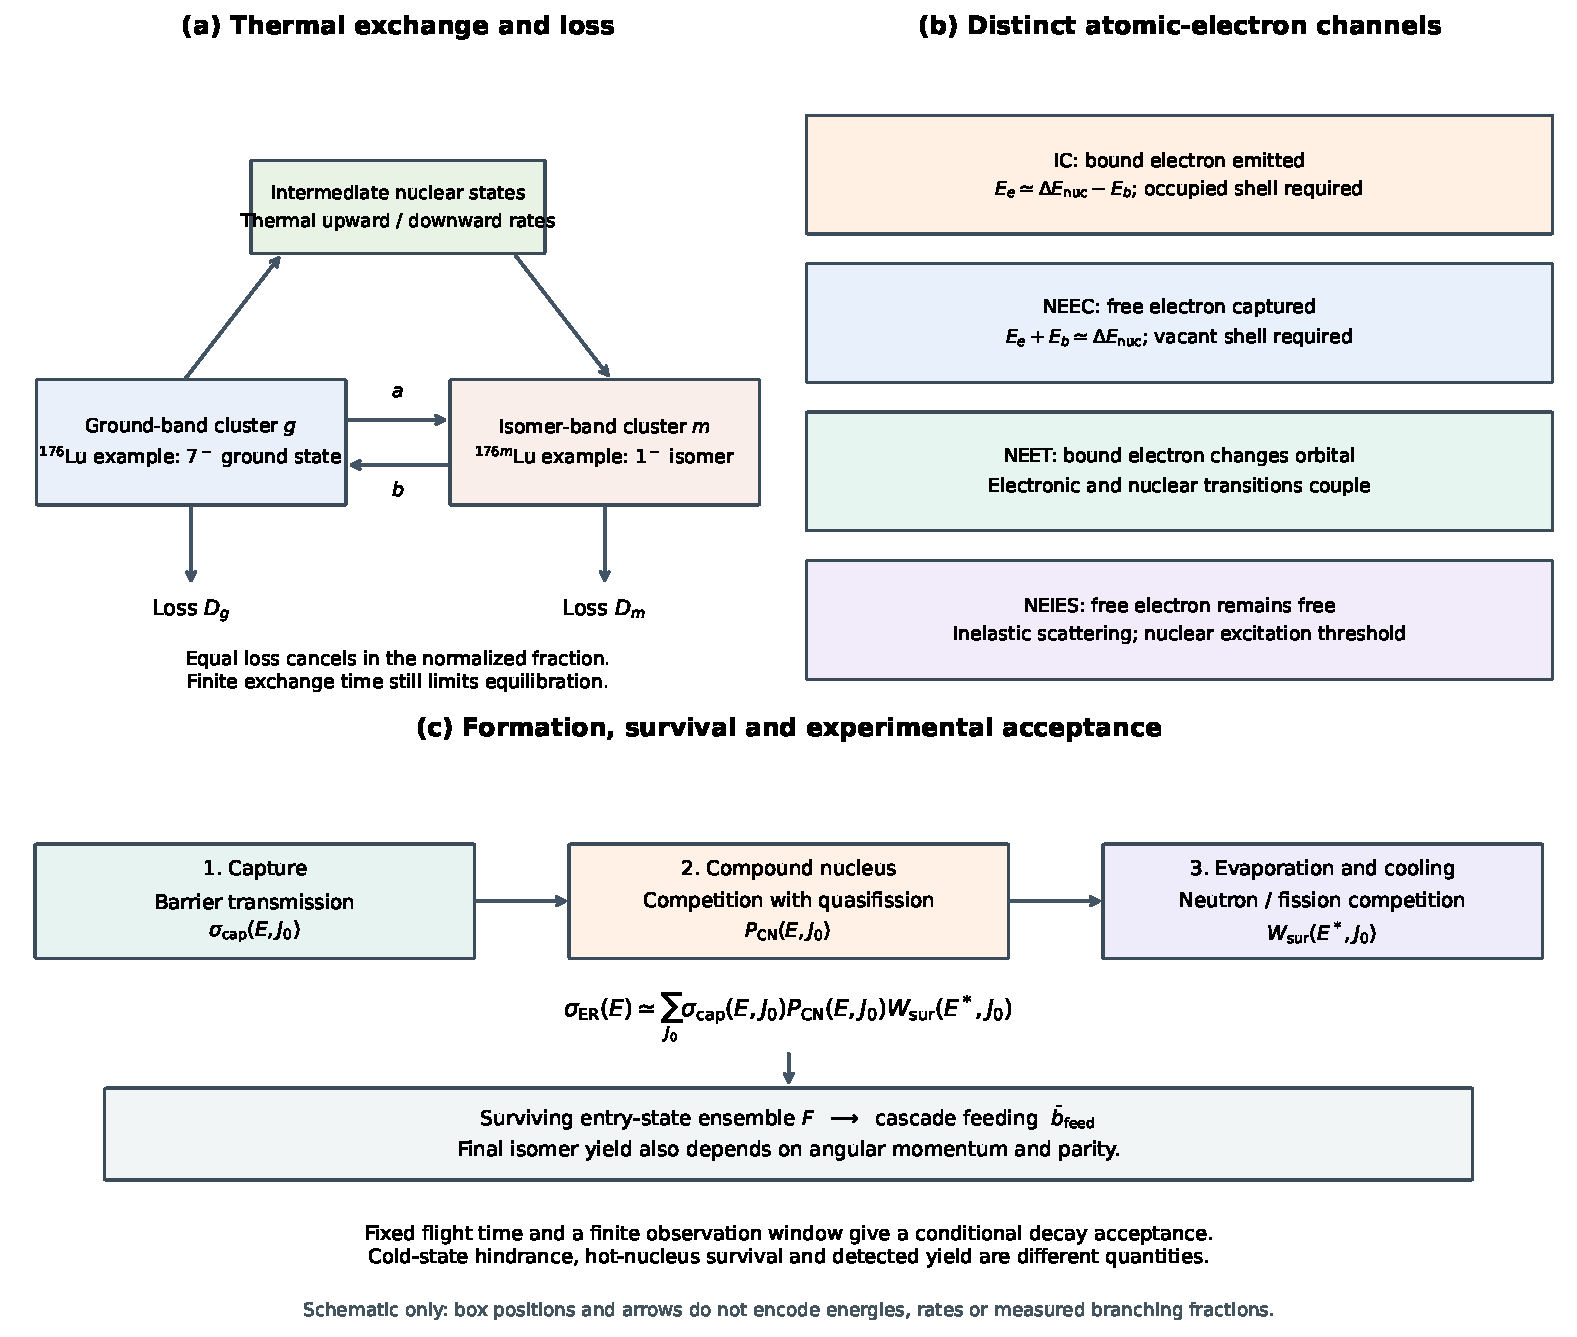
\includegraphics[width=0.98\textwidth]{Img/environment-network-pathways.pdf}
\caption[环境热浴、电子通道与重离子熔合形成对原子核可见性的重塑机制示意图]{环境热浴、电子通道与重离子熔合形成对原子核可见性的重塑机制示意图。(a) 天体热辐射浴中由中间桥态 $|i\rangle$ 介导的基态簇 $g$ 与异能态簇 $m$ 的有效交换网络与本征弛豫尺度；(b) 原子核与核外电子通道的微观竞争机制，包括内转换（IC）、电子俘获核激发（NEEC）、电子跃迁核激发（NEET）与非弹性电子散射（NEIES）；(c) 重离子完全熔合蒸发反应的三阶段分波框架（入射道俘获 $\sigma_{\mathrm{cap}}$、复合核形成 $P_{\mathrm{CN}}$、逐级退激存活 $W_{\mathrm{sur}}$）与进入态系综对异能态的馈入。}\label{fig:4-8-environment-network}
\end{figure}

\subsection{热环境开放网络与有效存活}\label{sec:4-8-1}

在天体物理环境（如渐近巨星分支 AGB 恒星的氦燃烧壳层、$s$-过程核合成温区）中，等离子体温度通常达到 $T_8 \sim 1$--$3$（即 $10^8\ \mathrm{K}$，对应能量标度 $kT \sim 8.6$--$25.9\ \mathrm{keV}$），即 $T_9 \sim 0.1$--$0.3$（$10^9\ \mathrm{K}$）。在这样极端的热力学环境中，原子核浸润在高密度的 Planck 热辐射光子浴以及高温自由电子气体之中。

设某一核素内部存在 $M$ 个离散量子能级（包括基态、低激发态、长寿命异能态以及高激发中间态）。以 $\mathbf{N}(t) = (N_1(t), N_2(t), \dots, N_M(t))^T$ 表示各能级的粒子数密度布居向量（单位为 $\mathrm{cm}^{-3}$）。在恒星核反应网络中，整个原子核能级系统的演化服从一阶非齐次常微分方程组所描述的开放速率网络（Open Rate Network）：
\begin{equation}\label{eq:4-8-network-master}
\frac{d \mathbf{N}(t)}{dt} = \mathbf{A}(T, n_e, \dots) \mathbf{N}(t) + \mathbf{P}(t),
\end{equation}
其中 $\mathbf{P}(t) = (P_1(t), P_2(t), \dots, P_M(t))^T$ 为外部产生流密度向量（例如上一级核反应链或中子俘获对特定能级的直接馈入），而转移矩阵 $\mathbf{A}$ 包含了所有内部能级跃迁与外部破坏漏失：
\begin{equation}\label{eq:4-8-matrix-elements}
A_{ij} = \lambda_{j \to i} \quad (i \ne j), \qquad
A_{ii} = -\sum_{j \ne i} \lambda_{i \to j} - d_i^{\mathrm{sink}}.
\end{equation}
矩阵元具有明确的物理意义与数学约束：
\begin{itemize}
\item \textbf{非对角元的非负性}：对于所有 $i \ne j$，$A_{ij} \ge 0$，表示从能级 $j$ 向能级 $i$ 跃迁的单向速率常数（单位为 $\mathrm{s}^{-1}$）。该跃迁率由光共振吸收、受激/自发辐射以及电子诱发过程共同贡献。
\item \textbf{对角元的外流与漏失}：对角项 $A_{ii} \le 0$ 由流向其他内部能级的总跃迁率以及向核素外部的净漏失率 $d_i^{\mathrm{sink}}$ 构成：
\begin{equation}\label{eq:4-8-sink-def}
d_i^{\mathrm{sink}} \equiv \lambda_{\beta^-}^{(i)} + \lambda_{\beta^+}^{(i)} + \lambda_{\mathrm{EC}}^{(i)} + \lambda_{(n,\gamma)}^{(i)} + \dots \ge 0.
\end{equation}
在此，$d_i^{\mathrm{sink}}$ 包含了从该能级出发导致原子核种类发生改变的所有不可逆弱衰变或核反应通道。
\item \textbf{列和与总核素数密度演化}：对矩阵 $\mathbf{A}$ 的每一列求和可知：
\begin{equation}\label{eq:4-8-column-sum}
\sum_{i=1}^M A_{ij} = A_{jj} + \sum_{i \ne j} A_{ij} = -\left(\sum_{i \ne j} \lambda_{j \to i} + d_j^{\mathrm{sink}}\right) + \sum_{i \ne j} \lambda_{j \to i} = -d_j^{\mathrm{sink}} \le 0.
\end{equation}
对式~\eqref{eq:4-8-network-master}在所有能级上求和，可得总核素数密度 $N_{\mathrm{tot}}(t) = \sum_i N_i(t)$ 的演化方程：
\begin{equation}\label{eq:4-8-total-pop-rate}
\frac{d N_{\mathrm{tot}}}{dt} = -\sum_{i=1}^M d_i^{\mathrm{sink}} N_i(t) + \sum_{i=1}^M P_i(t).
\end{equation}
在系统内部闭合（所有态的外部漏失率均为零，$d_i^{\mathrm{sink}} = 0$）且无外源产生（$\mathbf{P} = 0$）时，转移矩阵每一列和严格为零（$\sum_i A_{ij} = 0$），总核素粒子数密度对任意初值构型均严格守恒。闭合无外源是系统总粒子数对任意初值构型均守恒的充分物理条件；在开放反应网络中，若外部总产生率与总漏失率恰好处于动态平衡（$\sum_i P_i = \sum_i d_i^{\mathrm{sink}} N_i$），特定演化轨迹亦可呈现瞬时变化率为零的平衡态。若要求对于固定的非负常数项 $\mathbf{P}$ 与漏失率 $d_i^{\mathrm{sink}}$，在任意非负初始布居 $\mathbf{N}(0)$ 下均恒有 $d N_{\mathrm{tot}}/dt = 0$，则必须同时具备 $\mathbf{P} = 0$ 且对所有态 $d_i^{\mathrm{sink}} = 0$。
\end{itemize}

在热力学温度为 $T$ 的平衡辐射浴中，能量为 $\Delta = E_u - E_l$ 的光子平均占据数由 Bose-Einstein 统计给出：
\begin{equation}\label{eq:4-8-planck-dist}
n_\gamma(\Delta) = \frac{1}{\exp\left(\frac{\Delta}{kT}\right) - 1}.
\end{equation}
需要指出，$n_\gamma(\Delta)$ 表示每个电磁相空间模的平均光子占据数。在低能极限下（$\Delta \ll kT$），$n_\gamma \approx kT/\Delta$ 可以显著大于 1，不应将其误解为小于等于 1 的概率。

从高能级 $|u\rangle$ 向低能级 $|l\rangle$ 的退激过程由自发辐射与受激辐射共同贡献，其实际总退激跃迁率为：
\begin{equation}\label{eq:4-8-down-trans-rate}
\lambda_{u \to l} = A_{ul} \left[ 1 + n_\gamma(\Delta) \right] = A_{ul} \frac{\exp\left(\frac{\Delta}{kT}\right)}{\exp\left(\frac{\Delta}{kT}\right) - 1}.
\end{equation}
与之对应，从低能级 $|l\rangle$ 吸收环境光子跃迁至高能级 $|u\rangle$ 的光共振吸收跃迁率，由 Einstein 吸收系数与辐射场光子相空间密度导出：
\begin{equation}\label{eq:4-8-up-trans-rate}
\lambda_{l \to u} = \frac{2J_u + 1}{2J_l + 1} A_{ul} n_\gamma(\Delta) = \frac{2J_u + 1}{2J_l + 1} A_{ul} \frac{1}{\exp\left(\frac{\Delta}{kT}\right) - 1}.
\end{equation}
将式~\eqref{eq:4-8-up-trans-rate}与式~\eqref{eq:4-8-down-trans-rate}直接相除，即可得到成对电磁跃迁率的比例关系：
\begin{equation}\label{eq:4-8-detailed-balance-em}
\frac{\lambda_{l \to u}}{\lambda_{u \to l}} = \frac{2J_u + 1}{2J_l + 1} \exp\left(-\frac{\Delta}{kT}\right) = \frac{2J_u + 1}{2J_l + 1} \exp\left(-\frac{E_u - E_l}{kT}\right).
\end{equation}

式~\eqref{eq:4-8-detailed-balance-em}表述的是在 Planck 热辐射浴中，成对可逆电磁跃迁所严格遵循的微观详细平衡。然而，这一局域关系并不能等同于整个开放原子核网络必然服从宏观热平衡或全局 Boltzmann 统计分布：
\begin{equation}\label{eq:4-8-boltzmann-naive}
\frac{N_m}{N_g} \stackrel{?}{=} \frac{2J_m + 1}{2J_g + 1} \exp\left(-\frac{E_m - E_g}{kT}\right).
\end{equation}
全局平衡的破坏主要源于以下机制：
\begin{enumerate}
\item \textbf{非对称弱衰变漏失}：基态与异能态的核自旋、宇称与内部波函数构型往往存在剧烈差异，导致二者的 $\beta$ 衰变或电子俘获速率相差数个至十数个数量级（即 $d_g^{\mathrm{sink}} \ne d_m^{\mathrm{sink}}$）。弱衰变是向体系外部连续排泄布居的单向不可逆流动，破坏了全网络的封闭性。
\item \textbf{外源非平衡馈入}：上一级核反应链（例如中子俘获反应 $(n,\gamma)$）对各能级的馈入截面并不服从温度 $T$ 的热力学配分，而是由中子共振能级波函数决定（即 $P_g(t) / P_m(t)$ 不等于热平衡权重）。
\item \textbf{跨带耦合速率与有限热化时间}：带内能级由于较强的电磁跃迁，在光子浴驱动下可较快建立局域热平衡；但低自旋基态与高自旋（或大 $K$ 差）异能态之间的直接电磁跃迁受到强烈禁戒。两态之间的热交换必须依赖能量更高的非禁戒中间桥态进行多步跃迁，其有效交换速率有限。如果恒星环境温度演化时间尺度或核素破坏时间尺度短于跨带热化时间尺度，系统将始终处于动力学偏离平衡状态。
\item \textbf{弱相互作用透明性条件}：在典型 $s$-过程恒星演化壳层中，中微子平均自由程远大于恒星核尺寸，中微子流自由逸出，逆中微子吸收过程可以忽略；而在超新星坍缩等中微子不透明致密环境中，中微子相空间分布将直接介入反应网络，需要额外计入弱相互作用的非平衡输运。
\end{enumerate}

在物理上，我们可以将属于基态转动带的所有快速热平衡能级归并为基态簇（Ground Cluster，总布居记为 $N_g$），将属于异能态转动带的所有能级归并为异能态簇（Isomer Cluster，总布居记为 $N_m$）。带内能级由于纳秒或亚纳秒级的电磁退激，在高温光子浴提供充足向上激发的条件下可迅速建立局域热配分分布。定义有效跨簇交换率 $a \equiv \lambda_{g \to m}^{\mathrm{eff}}$ 与 $b \equiv \lambda_{m \to g}^{\mathrm{eff}}$，以及各簇的热加权有效破坏漏失率 $D_g$ 与 $D_m$（主要由各态的 $\beta$ 衰变贡献），双簇开网络方程可写为：
\begin{equation}\label{eq:4-8-two-cluster-master}
\frac{d}{dt}\begin{pmatrix} N_g(t) \\ N_m(t) \end{pmatrix} =
\begin{pmatrix} -(a + D_g) & b \\ a & -(b + D_m) \end{pmatrix}
\begin{pmatrix} N_g(t) \\ N_m(t) \end{pmatrix} +
\begin{pmatrix} P_g(t) \\ P_m(t) \end{pmatrix}.
\end{equation}

在恒定环境条件且无外部连续产生（$\mathbf{P} = 0$）的条件下，式~\eqref{eq:4-8-two-cluster-master}的演化由双态有效转移矩阵的特征值决定。设解的形式包含衰减因子 $e^{-r t}$，特征方程给出两个衰减特征值 $r_\pm$：
\begin{equation}\label{eq:4-8-cluster-eigenvalues}
r_\pm = \frac{1}{2}\left\{ (a + b + D_g + D_m) \pm \sqrt{(a + D_g - b - D_m)^2 + 4ab} \right\}.
\end{equation}
对式~\eqref{eq:4-8-cluster-eigenvalues}进行深入的物理极限与时间尺度分析：
\begin{enumerate}
\item \textbf{等漏失极限下的热化时间尺度}：当两簇的外部漏失率相等（$D_g = D_m = D$）时，根号内部化简为 $\sqrt{(a-b)^2 + 4ab} = a+b$。此时两个特征值为：
\begin{equation}\label{eq:4-8-lossless-limits}
r_- = D, \qquad r_+ = a + b + D.
\end{equation}
特征值之差严格为 $r_+ - r_- = a + b$。此时系统的总数按共同速率 $D$ 衰减，若考察归一化相对布居份额 $f \equiv N_m / (N_g + N_m)$，直接由式~\eqref{eq:4-8-two-cluster-master}求导可知 $D$ 项在归一化方程中严格相消：
\begin{equation}\label{eq:4-8-normalized-fraction-ode}
\frac{df}{dt} = a - (a + b)f - (D_m - D_g)f(1 - f) + \frac{P_m - f(P_g + P_m)}{N_{\mathrm{tot}}}.
\end{equation}
当 $D_g = D_m$ 且 $\mathbf{P} = 0$ 时，非线性选择项与外源项同时为零，归一化份额 $f(t)$ 严格按速率 $a + b$ 指数弛豫至平衡比 $a/(a+b)$。因此，在等漏失条件下，特征热化平均时间尺度表示为：
\begin{equation}\label{eq:4-8-therm-timescale}
\tau_{\mathrm{therm}} = \frac{1}{a + b} = \frac{1}{\lambda_{g \to m}^{\mathrm{eff}} + \lambda_{m \to g}^{\mathrm{eff}}},
\end{equation}
其对应的半平衡时间为 $t_{1/2}^{\mathrm{therm}} = \tau_{\mathrm{therm}} \ln 2 = \frac{\ln 2}{a + b}$。
严格闭合无损失的体系（$D_g = D_m = 0$）是该极限中 $r_- = 0$ 的充分特例，但并非唯一的物理适用条件。在常系数矩阵（恒温）且无外源（$\mathbf{P} = 0$）条件下，即便两簇存在非对称漏失（$D_g \ne D_m$），该线性自治系统仍可通过特征值与特征向量解析展开为 $\mathbf{N}(t) = \exp(\mathbf{A}t)\mathbf{N}_0$；然而此时系统的慢衰减特征模将偏离简单的 $a+b$。若环境温度随时间演化导致转移矩阵时变 $\mathbf{A}(t)$，或存在随时间变化的外源馈入流 $\mathbf{P}(t)$，系统将成为非自治微分方程组，瞬时单一有效寿命通常不足以描述整体布居动力学，应求解完整网络（数值求解或适当的解析卷积）。
\item \textbf{快速热化弱漏失极限下的有效衰变率}：当温度升高使得通过桥态的热激发交换率远大于两簇的弱衰变差异（即 $a + b \gg |D_g - D_m|$）时，较小特征值 $r_-$ 可以通过关于漏失差的微扰展开近似为：
\begin{equation}\label{eq:4-8-effective-decay-approx}
r_- \simeq D_{\mathrm{eff}} = \frac{b D_g + a D_m}{a + b}.
\end{equation}
在此极限下，成对电磁跃迁建立微观详细平衡，跨簇有效交换率之比趋向于簇配分函数加权比：
\begin{equation}\label{eq:4-8-partition-ratio}
\frac{a}{b} = \frac{\lambda_{g \to m}^{\mathrm{eff}}}{\lambda_{m \to g}^{\mathrm{eff}}} \simeq \frac{Z_m(T)}{Z_g(T)} \exp\left(-\frac{E_m - E_g}{kT}\right),
\end{equation}
其中 $Z_g(T) = \sum_{j \in g} (2J_j + 1) e^{-(E_j - E_g)/kT}$ 与 $Z_m(T) = \sum_{k \in m} (2J_k + 1) e^{-(E_k - E_m)/kT}$ 分别为基态簇与异能态簇的内部配分函数。将式~\eqref{eq:4-8-partition-ratio}代入式~\eqref{eq:4-8-effective-decay-approx}，全系统的宏观有效衰变破坏率表现为热加权平均形式：
\begin{equation}\label{eq:4-8-therm-decay-average}
D_{\mathrm{eff}}(T) \simeq \frac{Z_g(T) D_g + Z_m(T) e^{-(E_m - E_g)/kT} D_m}{Z_g(T) + Z_m(T) e^{-(E_m - E_g)/kT}}.
\end{equation}
但必须指出，微扰条件 $a + b \gg |D_g - D_m|$ 仅保证了长时间渐近衰减率可展开为热加权形式 $D_{\mathrm{eff}}$；在有限的恒星脉冲温区或实验观测时间窗内，系统是否真正达到这一热平衡布居，还强烈依赖于初始注入条件在快模 $r_+$ 与慢模 $r_-$ 上的投影分布，以及跨带特征交换时间 $\tau_{\mathrm{therm}} = 1/(a+b)$ 相对天体流体冷却时间或反应时间的大小。如果交换时间长于环境演化时间，原子核在尚未建立热平衡之前就可能已经发生严重的不平衡衰变漏失。
\end{enumerate}

天体核合成中一个代表性的理论模型实例是 $s$-过程核素 $^{176}\mathrm{Lu}$ 的跨带热化（Gintautas 等人 2009~\cite{gintautas-2009-176lu-thermal-equilibration}，Gosselin 等人 2010~\cite{gosselin-2010-plasma-isomers-176lu-180ta}）。在此需要强调，Gintautas 等人（2009）是基于 ENSDF 评估能级参数开展的跃迁速率与 $K$ 混合理论模型计算，而非给出新的直接实验测定。根据该文原件核定（PDF 第2页第II节开头），$^{176}\mathrm{Lu}$ 的基态为 $J^\pi = 7^-$（$K^\pi = 7^-$），具有长达 $T_{1/2} = 3.76 \times 10^{10}\ \mathrm{yr}$（平均寿命 $\tau \approx 5.42 \times 10^{10}\ \mathrm{yr}$）的弱衰变半衰期；而其激发能为 $122.9\ \mathrm{keV}$ 的同核异能态 $^{176m}\mathrm{Lu}$ 自旋宇称为 $J^\pi = 1^-$（$K^\pi = 0^-$），主要通过 $\beta^-$ 衰变到 $^{176}\mathrm{Hf}$（根据 NNDC/ENSDF 评估数据集~\cite{nndc-176lu-beta-2006-snapshot}，优势分支馈入 $^{176}\mathrm{Hf}$ 的 $0^+$ 基态与 $88.4\ \mathrm{keV}$ $2^+$ 能级，分支比分别约为 $39(2)\%$ 与 $61(2)\%$；由 $1^-$ 母态出发因宇称改变，属于一阶禁戒非唯一型跃迁，而非允许 Gamow-Teller 跃迁；此外存在向高激发负宇称态的极微弱允许分支与微小电子俘获分支），半衰期仅为 $T_{1/2} = 3.664\ \mathrm{h}$（平均寿命 $\tau \approx 5.29\ \mathrm{h}$）。在此体系中，基态具有高 $K$ 投影（$K=7$），而异能态为低 $K$ 态（$K=0$），二者自旋与 $K$ 投影的巨大差异使得电磁多极选择定则允许的两态间直接跃迁最低多极级次为 $E6$（$\Delta J = 6$，宇称不变），具有一级 $K$ 禁戒（$\nu = \Delta K-\lambda = 7-6=1$），并受到高多极辐射的强抑制（这属于跃迁多极级次的下界选择定则，与实验上直接测定纯 $E6$ 跃迁存在本质区别；在实际热平衡模型中直接跃迁均作可忽略近似）。在直接跃迁被强烈阻碍的前提下，两态之间的热耦合主要依赖高激发能量下的中间桥态（例如 Gintautas 等人原件 PDF 第2页明确指出的 $E_x = 838.6\ \mathrm{keV}$ 处的 $J^\pi = 5^-$、$K^\pi = 4^-$ 态）。
在冷恒星环境（$T_8 \lesssim 1$）中，光子浴无法有效激发至桥态，交换速率远小于异能态衰变率（$a, b \ll D_m$），基态与异能态在相关时间尺度内可近似分别演化，$^{176}\mathrm{Lu}$ 基态可作为测定星系核合成年龄的长寿命宇宙时钟；而在渐近巨星分支（AGB）恒星的热脉冲氦燃烧壳层（$T_8 \sim 2$--$3$）中，通过中间桥态的热光子共振吸收剧烈加速，特征热化时间 $\tau_{\mathrm{therm}} = 1/(a+b)$ 可以明显缩短，其数值仍取决于所采用的桥态参数及温度轨迹。根据式~\eqref{eq:4-8-therm-decay-average}，短寿命异能态的成分被强烈掺混到体系中，使得 $^{176}\mathrm{Lu}$ 的有效寿命在高温下缩短多个数量级，从而从“静态宇宙时钟”转变为灵敏探测恒星 $s$-过程环境温度的热力学温度计。

\subsection{原子与核电子通道微观解构}\label{sec:4-8-2}

在核多体理论中，激发态 $|i\rangle$ 向末态 $|f\rangle$ 在自由空间（真空）中的自发辐射跃迁率 $\lambda_{\gamma, if}$ 由跃迁能量 $E_\gamma = E_i - E_f$ 与约化跃迁几率 $B(\sigma L)$ 决定。在 SI 单位制与 Suhonen 电荷型磁算符体系下，自由空间多极辐射率标准式表示为：
\begin{equation}\label{eq:4-8-radiative-rate-standard}
\lambda_\gamma(\sigma L) = \frac{8\pi (L+1)}{L [(2L+1)!!]^2} \frac{1}{4\pi\varepsilon_0 \hbar} \left(\frac{E_\gamma}{\hbar c}\right)^{2L+1} B(\sigma L; I_i \to I_f).
\end{equation}
需要注意，式~\eqref{eq:4-8-radiative-rate-standard}属于真空自由空间定式；当原子核置于介电晶格等宏观介质中时，光子态密度的局域场修正将改变有效辐射率。对于真空磁偶极 $M1$ 跃迁（$L=1$），对应的自发辐射能级宽度 $\Gamma_\gamma = \hbar \lambda_\gamma$ 为：
\begin{equation}\label{eq:4-8-gamma-m1-width}
\Gamma_\gamma(M1) = \frac{16\pi}{9} \frac{1}{4\pi\varepsilon_0} \left(\frac{E_\gamma}{\hbar c}\right)^3 B_S(M1).
\end{equation}
若引入按各自基准单位归一化的无量纲数值 $b_{M1} \equiv B_S(M1) / (\mu_N/c)^2$（等价于 $B_\mu(M1) / \mu_N^2$），则实用跃迁率常数表示为：
\begin{equation}\label{eq:4-8-m1-practical-rate}
\lambda_\gamma(M1) = C_{M1} \left(\frac{E_\gamma}{\mathrm{MeV}}\right)^3 b_{M1}, \qquad C_{M1} \approx 1.7584 \times 10^{13}\ \mathrm{s}^{-1}.
\end{equation}
在物理计算中，两套单位体系中的无量纲纯数值 $b_{M1}$ 完全恒等，不可对已归一的数值重复乘除光速因子 $c^2$。

在给定环境条件下，处于固定激发初态 $|i\rangle$ 的原子核的总衰变宽度 $\Gamma_{\mathrm{tot}}^{(i)}$ 与实验寿命 $\tau_i = \hbar / \Gamma_{\mathrm{tot}}^{(i)}$（半衰期 $T_{1/2}^{(i)} = \tau_i \ln 2$），是由该初态向所有能量更低的开放末态 $|f\rangle$ 的自发退激与不可逆漏失通道共同决定的物理量：
\begin{equation}\label{eq:4-8-tot-width-decompose}
\Gamma_{\mathrm{tot}}^{(i)} = \sum_{f} \Gamma_{\gamma, if} \left(1 + \alpha_{if}\right) + \Gamma_{\mathrm{loss}}^{(i)},
\end{equation}
这里的求和针对可用光子分宽与内转换系数配对表示的多极支路；若还存在无单光子对应的 $E0$ 退激或其他非辐射通道，须另加相应分宽。其中 $\alpha_{if} \equiv \Gamma_{\mathrm{IC}, if} / \Gamma_{\gamma, if}$ 为各分通道的内转换系数，$\Gamma_{\mathrm{loss}}^{(i)}$ 包含了来自该初态的弱衰变或自发核裂变等不可逆向外排泄通道。当存在单一主导跃迁通道时，式~\eqref{eq:4-8-tot-width-decompose}常简化为 $\Gamma_\gamma(1 + \alpha_{\mathrm{IC}})$。必须强调，$\Gamma_{\mathrm{tot}}^{(i)}$ 严格表示固定初态 $|i\rangle$ 的\textbf{单向退激与漏失总和}；由外部自由电子俘获（NEEC）或强激光/等离子体驱动的向激发态的向上泵浦与布居重分配，属于开放动力学驱动过程，应当纳入式~\eqref{eq:4-8-network-master}所描述的速率网络主方程中进行整体演化求解，而不能混同为核单态固有的下行退激宽度。

在微观上，原子核与核外电子之间的相互作用通道包括以下不同物理过程：
\begin{itemize}
\item \textbf{自发辐射（$\gamma$）}：核初态通过量子真空电磁涨落发射单个实光子退激至末态，无需核外电子参与。
\item \textbf{内部转换（Internal Conversion, IC）}：激发态原子核通过虚光子交换将其跃迁能量传递给束缚态电子（结合能为 $E_b$）。该电子吸收能量后被电离并发射至连续谱，在忽略原子核/离子反冲动能以及环境介质能移的良好近似下，出射电子动能满足：
\begin{equation}\label{eq:4-8-ic-energy-cons}
E_e \approx \Delta E_{\mathrm{nuc}} - E_b > 0.
\end{equation}
内部转换通道的开放不仅要求跃迁能量大于电子结合能（$\Delta E_{\mathrm{nuc}} > E_b$），还严格要求对应的原子壳层存在实际被占有的电子。若原子处于高电离态（例如在重离子储存环或电子束离子阱 EBIT 中被剥离为全裸离子），内转换通道将因缺乏束缚电子而完全关闭，从而使有效辐射寿命延长数个数量级。需要指出，内转换系数并不普遍服从某一简单的幂律分布（如不可假定 $\alpha_{\mathrm{IC}} \propto E^{-(L+0.5)}$ 在任意低能区均成立），而高度依赖于电子波函数在核区的相对论重叠。因此不能无条件断言任意低能跃迁必定以内转换为主导。
\item \textbf{电子俘获核激发（Nuclear Excitation by Electron Capture, NEEC）}：微观上为内部转换过程的时间反演逆过程。一个处于连续谱、具有动能 $E_e$ 的自由电子，被具有内层空穴的离子所捕获，落入结合能为 $E_b$ 的束缚态空轨道中；释放的能量通过虚光子耦合传递给原子核，将核从初态 $|i\rangle$（基态或长寿命异能态）共振激发到触发能级 $|t\rangle$。在忽略离子反冲动能与环境微小频移的近似下，NEEC 过程要求入射连续自由电子动能与原子结合能之和匹配核能级差：
\begin{equation}\label{eq:4-8-neec-resonance-cond}
E_e + E_b \approx \Delta E_{\mathrm{nuc}} \equiv E_t - E_i.
\end{equation}
注意共振能量由初末核态的能量差 $\Delta E_{\mathrm{nuc}}$ 决定，而非异能态本身的绝对激发能。由于核能级与原子内层空穴均具有有限的自然宽度，NEEC 截面表现为具有有限宽度的 Breit-Wigner 共振峰，而非数学上的奇异点。
\item \textbf{非弹性电子散射核激发（Nuclear Excitation by Inelastic Electron Scattering, NEIES）}：处于连续谱的入射自由电子与原子核发生非弹性散射碰撞，出射电子依然留在连续谱中，并带走剩余动能 $E_e' = E_e - \Delta E_{\mathrm{nuc}}$。NEIES 是非共振的连续谱阈值过程，只要自由电子动能满足 $E_e > \Delta E_{\mathrm{nuc}}$ 即可开放。
\item \textbf{电子跃迁核激发（Nuclear Excitation by Electronic Transition, NEET）}：核外原子电子在束缚能级之间发生退激跃迁（例如由外层轨道跃迁至内层空穴），释放的跃迁能量通过虚光子耦合传递给原子核并将其激发。NEET 过程要求原子电子退激能量 $\Delta E_{\mathrm{el}}$ 与核激发能量 $\Delta E_{\mathrm{nuc}}$ 保持高度能量简并，且满足电磁多极选择定则。
\end{itemize}

为了具体阐明电子通道对物理可见性的改变，本节考察低能核物理领域的两个实验原件案例。

\subsubsection{案例一：$^{229}\mathrm{Th}$ 极低能异能态与光学核钟}

$^{229}\mathrm{Th}$ 拥有整个核素图谱中已知能量最低的同核异能态 $^{229m}\mathrm{Th}$（自旋宇称 $J^\pi = 3/2^+ [631]$，基态为 $5/2^+ [633]$），其核激发能量处于真空紫外波段（约 $8.34\ \mathrm{eV}$）。这一特殊的跃迁使 $^{229}\mathrm{Th}$ 成为制造高精度固态光学核钟的核心候选体系（Beeks 等人 2021~\cite{beeks-2021-thorium-229-isomer-nuclear-clock}）。

在中性自由 $^{229}\mathrm{Th}$ 原子环境中，钍原子的第一电离能约为 $I_1 \approx 6.3\ \mathrm{eV} < \Delta E_{\mathrm{nuc}}$，外层价电子的内转换通道完全开放且占据主导地位。Seiferle 等人（2017）在一项直接实验中，测得沉积在金属/微通道板表面环境下的中性 $^{229m}\mathrm{Th}$ 的内转换衰变半衰期为：
\begin{equation}\label{eq:4-8-seiferle-half-life}
T_{1/2}^{\mathrm{neutral}} = 7 \pm 1\ \mu\mathrm{s}
\end{equation}
（对应平均寿命 $\tau \approx 10\ \mu\mathrm{s}$；PRL 118, 042501，PDF p.~3，图2与图3）~\cite{seiferle-2017-lifetime-229th-isomer}。将其与理论预期的真空光子辐射寿命（$\tau_\gamma \sim 10^4\ \mathrm{s}$）对比，推导出内转换系数为 $\alpha_{\mathrm{IC}} \approx \tau_\gamma / \tau_{\mathrm{IC}} \sim 10^9$。这一寿命比较支持中性钍环境中内转换占优的解释，但需要明确 $\alpha_{\mathrm{IC}} \sim 10^9$ 是通过实测内转换半衰期与理论辐射寿命比较得出的推论参数，而非在中性钍实验中直接同时观测到了微弱的光子辐射分支。

随后，Kraemer 等人（2023）在欧洲核子中心 CERN-ISOLDE 将 $^{229}\mathrm{Ac}$ 植入宽带隙氟化物晶体（$\mathrm{MgF}_2$ 与 $\mathrm{CaF}_2$）中，直接观测到了该核态的光子辐射退激~\cite{kraemer-2023-radiative-decay-229th-isomer}。根据 Kraemer 等人原件（PDF 第3页），测得辐射波长为 $\lambda = 148.71 \pm 0.06_{\mathrm{stat}} \pm 0.41_{\mathrm{syst}}\ \mathrm{nm}$，对应跃迁能量为 $8.338 \pm 0.003_{\mathrm{stat}} \pm 0.023_{\mathrm{syst}}\ \mathrm{eV}$。在固体介质环境中，$\mathrm{CaF}_2$ 与 $\mathrm{MgF}_2$ 的晶体带隙分别高达 $12.1\ \mathrm{eV}$ 与 $12.4\ \mathrm{eV}$（Kraemer 等人 2023 原件 PDF 第2页），显著大于核激发能量，从而使得价带电子普通内转换在能量守恒上被有效抑制。Kraemer 等人在 $\mathrm{MgF}_2$ 晶体中直接测得的辐射退激半衰期为：
\begin{equation}\label{eq:4-8-th-rad-lifetime}
T_{1/2}(\mathrm{MgF}_2) = 670 \pm 102\ \mathrm{s}
\end{equation}
（对应晶体中平均寿命 $\tau \approx 967\ \mathrm{s}$；Nature 617, 706，PDF pp.~1, 3）~\cite{kraemer-2023-radiative-decay-229th-isomer}。在此需要明确两点物理边界：第一，式~\eqref{eq:4-8-th-rad-lifetime}是 $\mathrm{MgF}_2$ 宿主介质中的半衰期，不能将其混淆为 $\mathrm{CaF}_2$ 晶体中的数值或自由真空中的本征平均寿命；第二，晶体介质局域场效应改变了电磁场局域态密度，Kraemer 等人（原件 PDF 第4页）采用宏观折射率虚腔模型（$\mathrm{MgF}_2$ 在 $148.7\ \mathrm{nm}$ 处的折射率 $n = 1.488$，$n^3 \approx 3.3$）推导估算的真空辐射半衰期约为 $2.21(0.34) \times 10^3\ \mathrm{s}$，作者明确指出该宏观电介质连续介质修正对于离子浅表面植入的适用性存在局限，属于特定模型推论而非自由真空中的直接测量；此外宽带隙晶体抑制了理想价带的内转换，但晶格缺陷、色心或杂质能级引入的非辐射弛豫通道在实际材料中仍须作为实验不确定度保留。

\subsubsection{案例二：$^{93m}\mathrm{Mo}$ 异能态耗散与 NEEC 实验争议}

利用外来电子通道诱发长寿命异能态加速退激（Isomer Depletion），是核能受控释放与核电池研究关注的物理机制。在 $^{93}\mathrm{Mo}$ 中，基态为 $J^\pi = 5/2^+$，存在一个半衰期长达 $T_{1/2} = 6.85\ \mathrm{h}$（平均寿命 $\tau \approx 9.88\ \mathrm{h}$）的高自旋异能态 $^{93m}\mathrm{Mo}$（$J^\pi = 21/2^+$，$E_x = 2424.9\ \mathrm{keV}$）。在异能态上方 $5.5\ \mathrm{keV}$ 处存在一个触发能级（$J^\pi = 17/2^+$，$E_x = 2430.4\ \mathrm{keV}$，半衰期 $T_{1/2} = 3.5\ \mathrm{ns}$，对应平均寿命 $\tau \approx 5.05\ \mathrm{ns}$）。该能级可通过 $268\ \mathrm{keV}$ 跃迁迅速级联至基态。

围绕该核态是否能够通过 NEEC 过程实现诱发耗散，实验与理论物理界展开了深入检验：
\begin{enumerate}
\item \textbf{Chiara 等人（2018）的初次报道}：Chiara 等人在阿贡国家实验室 ATLAS 装置上利用 $^{7}\mathrm{Li}(^{90}\mathrm{Zr}, p3n)^{93m}\mathrm{Mo}$ 逆运动学重离子反应产生反冲离子，使其穿透碳减速薄膜~\cite{chiara-2018-mo93m-isomer-depletion-neec}。作者报道探测到了多普勒频移的 $2475\ \mathrm{keV}$ 馈入射线与未频移的 $268\ \mathrm{keV}$ 跃迁之间的符合计数，提取出的异能态耗散几率为：
\begin{equation}\label{eq:4-8-chiara-value}
P_{\mathrm{exc}} = 0.010(3) \quad (\text{即 } 1.0 \pm 0.3\%)
\end{equation}
（Nature 554, 216，PDF pp.~2, 5），并将其归因为离子在慢化过程中捕获自由电子诱发的 NEEC 过程。
\item \textbf{Wu 等人（2019）的相对论原子理论计算}：Wu、Keitel 与 P\'alffy（2019）在 PRL 发表了针对该慢化过程的理论模拟~\cite{wu-2019-mo93m-neec-stopping-theory}。结合多组态 Dirac-Fock 波函数与 CasP 离子阻止本领模型，作者追踪了 $^{93m}\mathrm{Mo}$ 离子穿过碳膜慢化过程中的电荷态演化与 648 个共振捕获通道。理论计算给出的总耗散几率仅为：
\begin{equation}\label{eq:4-8-wu-theory-value}
P_{\mathrm{exc}}^{\mathrm{theory}} \approx (2.26\text{--}2.73) \times 10^{-11},
\end{equation}
与 Chiara 等人的实验报告相差约 9 个数量级。
\item \textbf{Guo 等人（2021）提出的本底污染竞争解释}：Guo 等人在 Nature 发表评论指出~\cite{guo-2021-mo93m-depletion-contamination-challenge}，在重离子熔合反应靶点附近，极强的瞬发 $\gamma$ 级联、靶杂质反应以及密集本底计数可能通过假符合模拟出微弱的 $268\ \mathrm{keV}$ 峰；Chiara 等人随后在回复中对符合门设置与本底扣除进行了辩护。
\item \textbf{Guo 等人（2022）兰州 HIRFL/RIBLL 次级异能束实验}：为了彻底隔离初级核反应靶点的强辐射本底，Guo 等人（2022）在兰州重离子加速器国家实验室（HIRFL）的放射性束流线（RIBLL，35 米输运线）上开展了独立检验~\cite{guo-2022-mo93m-isomer-beam-depletion-limit}。实验采用 $^{12}\mathrm{C}(^{86}\mathrm{Kr}, 5n)$ 初级反应与 $559\ \mathrm{MeV}$ 初级束流，在测量端获得了动能为 $460\ \mathrm{MeV}$ 的 $^{93m}\mathrm{Mo}^{36+}$ 次级离子束（异能态纯度约为 $0.6\%$）。在将该束流注入碳慢化靶后，作者在 $266.5$--$269.5\ \mathrm{keV}$ 能窗内观测到 570 计数（对应 Compton 本底估计为 596 计数，$3\sigma$ 下限为 523 计数），未观测到统计显著的 $268\ \mathrm{keV}$ 净发射峰。在考虑中心 $3\ \mathrm{keV}$ 能窗对假设高斯峰形具有 $95\%$ 的面积接受度（acceptance，用以将窗内缺失的高斯边缘面积折算回全峰面积）后，提取出净峰计数上限约为 $(570 - 523)/95\% \sim 50$ 计数，进而确立激发几率上限为：
\begin{equation}\label{eq:4-8-guo-limit-value}
P_{\mathrm{exc}}^{\mathrm{exp}} < 2 \times 10^{-5}
\end{equation}
（PRL 128, 242502，PDF pp.~3--4，式(1)--(3)）~\cite{guo-2022-mo93m-isomer-beam-depletion-limit}。需要明确，原件中的 $95\%$ 是能量积分窗对假设高斯峰面积的截断接受比例，而不是最终上限 $P_{\mathrm{max}} \approx 2 \times 10^{-5}$ 的统计置信度（后者在推导中结合了本底计数的 $3\sigma$ 下限构造）。
\end{enumerate}

Guo 等人（2022）在兰州 RIBLL 获得的 $2 \times 10^{-5}$ 上限比 Chiara 等人早先声称的 $1\%$ 降低了 500 倍，对原实验在减速介质中观测到宏观大截面耗散的结论构成了直接质疑。同时，评价该结果需要保持客观的物理边界：该上限是在特定束流能量（$460\ \mathrm{MeV}$）、电荷态（$36^+$）与固体碳靶减速条件下测得的，不能将其简单等同于在储存环或重离子阱等其他物理平台全面排除了 NEEC 过程的存在。这一学术争议表明，微观核过程的实验判据必须与原子电荷态演化及本底符合模型置于统一物理条件下进行交叉自洽检验。

\subsection{重离子完全熔合形成与存活几率}\label{sec:4-8-3}

在前述讨论中，我们探讨了核态在合成之后，如何在外部热场或电子环境中改变其有效寿命。而在在束实验谱学与超重核人工合成中，激发态是如何在反应中被实际产生出来的？长寿命异能态的冷态微观位垒是否意味着反应产生截面必定增大？本小节建立重离子完全熔合反应的分波框架，并对这些问题进行微观解构。

在质心系入射动能为 $E$ 时，合成特定蒸发剩余核的产生截面可对初始复合核总角动量 $J_0$ 进行分波展开：
\begin{equation}\label{eq:4-8-er-master}
\sigma_{\mathrm{ER}}(E) = \sum_{J_0=0}^\infty \sigma_{\mathrm{cap}}(E, J_0) P_{\mathrm{CN}}(E, J_0) W_{\mathrm{sur}}(E^*, J_0).
\end{equation}
公式中各项的物理意义如下：
\begin{itemize}
\item $\sigma_{\mathrm{cap}}(E, J_0)$ 为初始总角动量为 $J_0$ 时的部分俘获截面（Partial Capture Cross Section），其量纲为面积。对于自旋为零的弹靶体系（$I_1 = 0, I_2 = 0$），$J_0 = l$，部分俘获截面的标准表达式为：
\begin{equation}\label{eq:4-8-sigma-cap-spin0}
\sigma_{\mathrm{cap}}(E, J_0) = \frac{\pi \hbar^2}{2\mu E} (2J_0 + 1) T(E, J_0),
\end{equation}
其中 $\mu$ 为进入通道折合质量，$T(E, J_0)$ 为进入通道势垒穿透几率。需要注意，若 $\sigma_{\mathrm{cap}}(E, J_0)$ 的定义式中已经显式包含了统计权重因子 $(2J_0 + 1)$，在式~\eqref{eq:4-8-er-master}对 $J_0$ 的求和中不得再次乘入 $(2J_0+1)$。
\item 若弹核或靶核具有非零内禀基态自旋 $I_1$ 与 $I_2$，进入通道总通道自旋为 $\mathbf{S} = \mathbf{I}_1 + \mathbf{I}_2$，初始复合核总角动量为 $\mathbf{J}_0 = \mathbf{l} + \mathbf{S}$。在无极化的统计平均系综下，严格的部分俘获截面表示为：
\begin{equation}\label{eq:4-8-sigma-cap-general-spin}
\sigma_{\mathrm{cap}}(E, J_0) = \frac{\pi \hbar^2}{2\mu E} \frac{2J_0 + 1}{(2I_1 + 1)(2I_2 + 1)} \sum_{S=|I_1 - I_2|}^{I_1 + I_2} \sum_{l=|J_0-S|}^{J_0+S} T_{lS}^{J_0}(E).
\end{equation}
在穿透几率主要由离心位垒主导而对通道自旋耦合弱敏感的近似下，常将穿透矩阵元简化为仅依赖轨道角动量与总角动量的形式 $T_l(E, J_0)$，但不可在未声明近似的前提下将所有不同通道自旋构型混同为单一通道。
\item $P_{\mathrm{CN}}(E, J_0)$ 为无量纲条件概率，表示两核克服入射库仑势垒形成接触双核系统后，成功演化为空间紧致的单体复合核的几率。
\item $W_{\mathrm{sur}}(E^*, J_0)$ 为无量纲存活几率，表示初始激发能为 $E^*$、初始总角动量为 $J_0$ 的复合核在经历粒子蒸发并与裂变竞争后，最终存活为冷蒸发剩余核的几率。复合核初始激发能为：
\begin{equation}\label{eq:4-8-excitation-energy-def}
E^* = E - Q_{\mathrm{fus}}, \qquad Q_{\mathrm{fus}} \equiv M(C)c^2 - M(A_1)c^2 - M(A_2)c^2.
\end{equation}
\end{itemize}

在实际核反应理论中，式~\eqref{eq:4-8-er-master}中的三个因子分别由不同的微观物理机制所支配（Zagrebaev 等人 2001~\cite{zagrebaev-2001-superheavy-synthesis-survival}）：
\begin{enumerate}
\item \textbf{俘获阶段（$\sigma_{\mathrm{cap}}$）}：在近垒与次垒能区，势垒穿透几率受到多道耦合效应（Channel Coupling）的支配。弹靶核的低能集体转动（如四极形变 $\beta_2$、十六极形变 $\beta_4$）、表面低频振动以及核子转移通道，将一维静电势垒展开为多维结构。实验上常通过熔合激发函数二阶微分定义可操作的表观势垒分布 $D_{\mathrm{fus}}(E) = \frac{d^2(E \sigma_{\mathrm{fus}})}{dE^2}$。必须注意，该定义属于由截面曲率反演的唯象表观量，在存在强烈准裂变或复合核形成几率 $P_{\mathrm{CN}}(E)$ 具有显著能量依赖的重体系中，它并不等同于裸入射接触势垒的几何概率密度分布，不可混淆俘获截面、完全熔合截面与蒸发剩余截面的各自能量导数。
\item \textbf{复合核形成阶段（$P_{\mathrm{CN}}$）与体系依赖性}：接触后的双核系统在质量不对称度 $\eta = (A_1 - A_2)/(A_1 + A_2)$、伸长量与颈部厚度的多维势能面上耗散演化。对于较轻的中等质量体系（如某些 $Z_1 Z_2 \lesssim 1000$ 的反应例），双核系统接触后迅速演化为单核，$P_{\mathrm{CN}} \approx 1$。但在大库仑参数体系中（例如特定超重核合成反应通道，库仑乘积高达 $Z_1 Z_2 \gtrsim 1600$--$2000$ 的冷熔合或热熔合特定能区），系统面临强烈的准裂变（Quasifission, QF）竞争，导致在紧致单核形成之前即发生解体，使特定体系和能窗下的 $P_{\mathrm{CN}}$ 降至 $10^{-2}$--$10^{-4}$ 甚至更低量级。这些数值仅代表特定重核反应能窗的唯象模型示例，而非跨越全核区的普适常数，实际数值强烈取决于弹靶质量不对称度、入射动能及形变碰撞取向。
\item \textbf{去激发存活阶段（$W_{\mathrm{sur}}$）}：严格的多中子级联退激过程要求在每一蒸发步对出射中子连续动能能谱进行积分，并最终耦合终末 $\gamma$ 辐射退激冷却（Zagrebaev 等人 2001~\cite{zagrebaev-2001-superheavy-synthesis-survival}，PDF 第7页式(10)--(11)）。若采用代表性中心动能与离散中子发射假定，去激发存活几率可表达为常用的分宽比乘积近似：
\begin{equation}\label{eq:4-8-wsur-product}
W_{\mathrm{sur}}(E^*, J_0) \simeq \Delta_x(E^*, J_0) \prod_{k=1}^x \left[ \frac{\Gamma_n(E_k^*, J_k)}{\Gamma_{\mathrm{tot}}(E_k^*, J_k)} \right],
\end{equation}
其中 $\Delta_x(E^*, J_0)$ 为能量实现因子（例如 Jackson 因子），表示经历 $x$ 步蒸发后剩余激发能恰好落入粒子发射阈值与有效裂变位垒之下的 $\gamma$ 能窗的几率。此因子与第4.7节中弱衰变相关的 $\beta$ 缓发中子发射几率 $P_{xn}$ 具有不同的物理定义，不可混淆。总宽度 $\Gamma_{\mathrm{tot}} = \Gamma_n + \Gamma_f + \dots$ 中占主导竞争的是中子宽度 $\Gamma_n$ 与裂变宽度 $\Gamma_f$。

根据 Hauser-Feshbach 统计理论与 Bohr-Wheeler 裂变过渡态理论，中子蒸发宽度与裂变宽度分别表述为：
\begin{align}
\Gamma_n(E^*, J) &= \frac{1}{2\pi \rho(E^*, J)} \sum_{J'} \sum_{l, j_n} \int_0^{E^* - S_n} T_l(\epsilon) \rho_R(E^* - S_n - \epsilon, J') d\epsilon, \label{eq:4-8-gamma-n-stat}\\
\Gamma_f(E^*, J) &= \frac{1}{2\pi \rho(E^*, J)} \int_0^{E^* - B_f(J)} \rho_{\mathrm{saddle}}(E^* - B_f(J) - \epsilon) d\epsilon, \label{eq:4-8-gamma-f-stat}
\end{align}
其中 $S_n$ 为单中子分离能，$\rho_R$ 为残余核能级密度，$\rho_{\mathrm{saddle}}$ 为裂变鞍点过渡态能级密度，$\rho(E^*, J)$ 为初始激发态能级密度，而 $B_f(J)$ 为有效裂变位垒。在式~\eqref{eq:4-8-gamma-n-stat}与式~\eqref{eq:4-8-gamma-f-stat}中，分母中的能级密度量纲均为能量的倒数（$\mathrm{MeV}^{-1}$），分子积分项均为无量纲的开放通道数，因此两式给出的能级宽度均具有能量量纲（$\mathrm{MeV}$）。式~\eqref{eq:4-8-wsur-product}中各蒸发步的能量与角动量必须动态递推更新：
\begin{equation}\label{eq:4-8-stepwise-dyn-update}
E_k^* = E_{k-1}^* - S_n^{(k)} - \epsilon_k, \qquad \mathbf{J}_k = \mathbf{J}_{k-1} - \mathbf{j}_n^{(k)}.
\end{equation}
\end{enumerate}

在式~\eqref{eq:4-8-gamma-f-stat}中，决定中子与裂变竞争的关键物理量是有效裂变位垒 $B_f$。在微观--宏观模型中，总裂变位垒通常表示为宏观液滴位垒与裂变鞍点及基态处微观壳修正差值的叠加，其通用相减式为：
\begin{equation}\label{eq:4-8-shell-barrier-contrib}
B_f = B_f^{\mathrm{LD}} + \Delta B_f^{\mathrm{shell}}, \qquad \Delta B_f^{\mathrm{shell}} \equiv \delta U_{\mathrm{saddle}} - \delta U_{\mathrm{gs}}.
\end{equation}
需要指出，宏观液滴位垒并不能在整个超重或重核区普遍假设为零（例如在 Zagrebaev 等人 2001 原件 PDF 第7页第V.A节的 $^{254}\mathrm{No}$ 邻区计算例子中，宏观液滴位垒仍有约 $1.2\ \mathrm{MeV}$）；仅在某些极重、壳效应占绝对主导的核区，液滴位垒才降至极低水平。在此类壳稳定核体系中，基态量子壳修正使核结合能增加，对应质量亏损式中取负值（$\delta U_{\mathrm{gs}} < 0$）；而在鞍点处由于处于大伸长与颈部形变，单粒子壳效应受到强烈平均冲刷，唯象上常作 $\delta U_{\mathrm{saddle}} \approx 0$ 的近似处理，从而在此特定壳主导条件下导出净微观位垒增强为正值：
\begin{equation}\label{eq:4-8-shell-approx-positive}
\Delta B_f^{\mathrm{shell}} \approx -\delta U_{\mathrm{gs}} > 0.
\end{equation}
必须注意，$\delta U_{\mathrm{gs}} < 0$ 与 $\delta U_{\mathrm{saddle}} \approx 0$ 属于所论壳主导超重核体系的唯象近似，而非适用于任意轻核或过渡核的普遍数学定理。在唯象壳阻尼模型（Zagrebaev 等人 2001~\cite{zagrebaev-2001-superheavy-synthesis-survival}）中，有效裂变位垒随激发能的阻尼通常表达为：
\begin{equation}\label{eq:4-8-bf-shell-decomp}
B_f(E^*) = B_f^{\mathrm{LD}} + \Delta B_f^{\mathrm{shell}} \exp\left(-\gamma_D E^*\right),
\end{equation}
其中 $\gamma_D$ 为唯象壳阻尼参数。需要区分的是，Ignatyuk 原始模型是对 Fermi 气体单粒子能级密度参数 $a(E^*)$ 建立的能量阻尼方程，将该阻尼形式直接映射为裂变位垒的纯指数衰减属于宏观--微观统计模型的经验参数化处理，并不意味着所有超重核各分波的实际势垒变化均严格服从完全相同的指数曲线。当复合核初始激发能较高（例如热熔合反应中 $E^* \sim 30$--$50\ \mathrm{MeV}$）时，微观壳修正发生剧烈阻尼，有效裂变位垒显著衰减，导致蒸发链前几步的裂变相空间急剧膨胀，存活几率受到极大压制。

针对超重核高自旋同核异能态的稳定性，Xu 等人（2004）的研究表明，在超重核高 $K$ 多准粒子态中，费米面附近特定轨道的高自旋单核子准粒子激发会显著抬高局域势能面，从而在冷态下赋予异能态更高的自发裂变位垒~\cite{xu-2004-superheavy-high-spin-isomer-stability}。然而，冷态下的这种微观稳定性并不等同于在重离子熔合反应中该异能态的产生截面必定增大：
\begin{itemize}
\item \textbf{能量阶段与统计竞争的脱耦}：决定熔合蒸发剩余截面 $\sigma_{\mathrm{ER}}$ 的是复合核在高温激发能（$E^* \sim 30$--$50\ \mathrm{MeV}$）下的存活几率。在这一高激发能阶段，原子核处于统计连续能级密度谱中，壳修正根据式~\eqref{eq:4-8-bf-shell-decomp}经历显著阻尼，中子发射与裂变竞争由平均相空间能级密度积分决定，不能直接代入零温冷态下的离散异能态裂变位垒。
\item \textbf{进入态系综与馈入分支比}：复合核蒸发完全部中子降落到粒子阈值之下后，经过逐级动量与能量排放，在离散与准连续谱交界处形成分布在不同激发能与自旋上的进入态系综（Entry States Ensemble）。必须明确区分初始复合核的角动量 $J_0$ 与蒸发后实际到达的进入态角动量 $J_{\mathrm{entry}}$。设 $F(E_{\mathrm{entry}}^*, J_{\mathrm{entry}}, \pi \mid E, J_0, \mathrm{surv})$ 为初始具有总角动量 $J_0$ 的复合核在存活后到达具体进入态 $(E_{\mathrm{entry}}^*, J_{\mathrm{entry}}, \pi)$ 的条件归一化分布函数（满足 $\sum_{J_{\mathrm{entry}}, \pi} \int dE_{\mathrm{entry}}^* F = 1$）。由特定进入态通过统计与离散 $\gamma$ 级联汇入该异能态的分支比为 $b_{\mathrm{feed}}(E_{\mathrm{entry}}^*, J_{\mathrm{entry}}, \pi) \in [0, 1]$，则由初始分波 $J_0$ 级联汇入异能态的级联平均分支比为：
\begin{equation}\label{eq:4-8-bfeed-j0-def}
\bar{b}_{\mathrm{feed}}(E, J_0) \equiv \sum_{J_{\mathrm{entry}}, \pi} \int dE_{\mathrm{entry}}^* F(E_{\mathrm{entry}}^*, J_{\mathrm{entry}}, \pi \mid E, J_0, \mathrm{surv}) b_{\mathrm{feed}}(E_{\mathrm{entry}}^*, J_{\mathrm{entry}}, \pi).
\end{equation}
从而最终生成特定异能态的截面表示为对初始复合核分波 $J_0$ 的加权求和：
\begin{equation}\label{eq:4-8-isomer-feeding-ensemble}
\begin{aligned}
\sigma_{\mathrm{isomer}}(E) &= \sum_{J_0} \sigma_{\mathrm{cap}}(E, J_0) P_{\mathrm{CN}}(E, J_0) W_{\mathrm{sur}}(E^*, J_0) \bar{b}_{\mathrm{feed}}(E, J_0) \\
&= \sum_{J_0} \sigma_{\mathrm{ER}}(E, J_0) \bar{b}_{\mathrm{feed}}(E, J_0).
\end{aligned}
\end{equation}
在唯象讨论中常写的关系 $\sigma_{\mathrm{isomer}} \approx b_{\mathrm{eff}} \sigma_{\mathrm{ER}}$ 中，有效分支比：
\begin{equation}\label{eq:4-8-beff-def}
b_{\mathrm{eff}} \equiv \frac{\sum_{J_0} \sigma_{\mathrm{ER}}(E, J_0) \bar{b}_{\mathrm{feed}}(E, J_0)}{\sum_{J_0} \sigma_{\mathrm{ER}}(E, J_0)}
\end{equation}
严格是全分波剩余核产生截面加权的系综平均值（分母要求总剩余截面非零）。若反应进入通道角动量输入偏低，使得进入态系综的自旋分布无法有效重叠到高自旋异能态的侧线馈入带上，大部分级联流将旁路流向低自旋基态，使得该异能态的有效截面受到严重抑制。
\item \textbf{实验探测时间窗口与可观测性过滤}：合成后的核态能否在实验上被清晰辨识，受到谱学探测装置时间窗口的严格筛选。对于通过反冲质量分离器输运至焦平面进行“反冲--衰变关联”测量的实验构型，设离子在实验室系中的平均飞行时间为 $t_f$（典型约为 $1\ \mu\mathrm{s}$），焦平面探测器设置的后续电子学时间关联窗宽为 $\Delta t$。对于一个实验室寿命为 $\tau$（半衰期 $T_{1/2} = \tau \ln 2$）的核态，其在焦平面被成功关联探测的理想几何与衰变接受概率由两阶段生存与衰变几率决定：
\begin{equation}\label{eq:4-8-detection-acceptance-prob}
\mathcal{P}_{\mathrm{det}}(\tau) = \exp\left(-\frac{t_f}{\tau}\right) \left[ 1 - \exp\left(-\frac{\Delta t}{\tau}\right) \right] \cdot \epsilon_{\mathrm{decay}} \cdot \epsilon_{\mathrm{geom}},
\end{equation}
其中 $\epsilon_{\mathrm{decay}}$ 为特征衰变分支比，$\epsilon_{\mathrm{geom}}$ 为探测几何效率。式~\eqref{eq:4-8-detection-acceptance-prob}清楚表明了双侧抑制效应：当核态寿命远短于飞行时间（$\tau \ll t_f$）时，指数因子 $\exp(-t_f/\tau)$ 急剧趋近于零，核态在飞行途中发生在途衰变损失；而当寿命远长于电子学时间窗（$\tau \gg \Delta t$）时，括号内因子展开为 $\Delta t / \tau \ll 1$，时间窗内发生衰变的比例极低，导致偶然本底竞争加剧。需要说明的是，这种时间窗筛选属于特定焦平面关联谱学技术的几何与定时响应，它并不意味着超短寿命核态在物理上完全无法观测——利用紧邻反应靶放置的瞬发 $\gamma$ 探测器阵列、在束转换电子谱仪或在途飞行衰变谱仪（Decay-in-flight spectrometers），依然可以在不同实验构型下捕获这些短寿命态的特征辐射。
\end{itemize}

综上所述，原子核在零温真空下的内禀性质（长寿命、高禁戒度、高裂变位垒）与其在宏观天体环境中的有效存活性、在弱相互作用与外场中的退激演化以及在重离子核反应中的形成截面与实验可见性之间，存在着清晰的动力学物理台阶。在实验谱学与微观核结构分析中，必须将内禀矩阵元、外在介质环境与动力学反应机制区分推导，方能建立自洽且经受检验的物理结论。
%
}{%
    \section{环境和形成路径怎样改变可见性 [未完成]}\label{sec:4-8}%
    \textit{本节尚未完成。}%
}
